\documentclass[10pt]{article}
\usepackage{graphicx,amssymb, amstext, amsmath, epstopdf, booktabs, 
verbatim, gensymb, geometry, appendix, natbib, lmodern, hyperref, float, titlesec, subfig}
\geometry{letterpaper}
%\usepackage{garamond}

\newcommand*\Title{Neurowrx Account Manual}
\newcommand*\cpiType{}
\newcommand*\Date{Novermber 2018}
\newcommand*\Author{Michael Braeutigam}
\title{Neurowrx Account Manual}
\author{Michael Braeutigam}
\date{\today}
%-----------------------------------------------------------

\usepackage{cpistuff/cpi} % This is what makes your document look like a cpi document.


\begin{document}

\begin{titlepage}
\maketitle
\end{titlepage}

\linespread{1.15} %Set standard document linespacing

\begin{executive}

This is a document describing the functionality of the neurowrx website.

\frame{
\textbf{Important Title}

This is a convenient place to put any necessary legal mumbo-jumbo}
\end{executive}

\tableofcontents


\section{Ordinary Members}

\subsection{Account Creation}

\begin{flushleft}
Once you are a neurowrx member, a username (probably based on your actual name, or organization name) will be chosen by the site admin, and you will receive an email at the address that you provided in your application.  It will have neurowrx in the subject line so check your spam filter if you do not receive it promptly.  It will notify you of your username and give you a link to a page where you can set your password, as well as a link to the regular login panel.  The login panel can be reached though this link or though the main site at \url{https://neurowrx.org/}, by clicking on the button at the top right corner. 
\end{flushleft}

\begin{figure}[h]
\centering
\caption{A typical account creation email}
\label{accountemail}
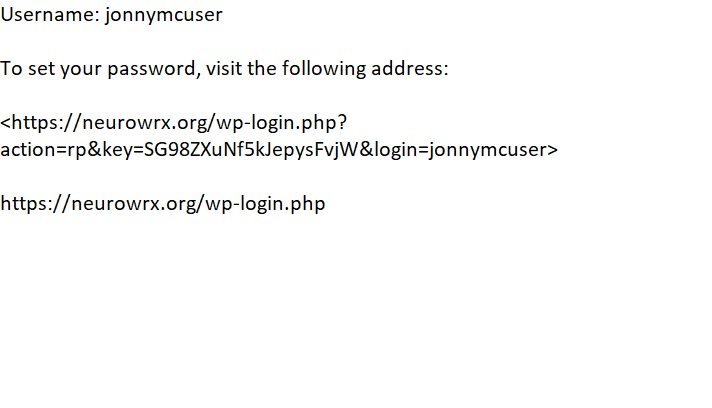
\includegraphics[scale=1.0]{images/accountcreation.jpg}
\end{figure}

The account's password is initially randomized and should be set via the first link before one attempts to log in.  In the case that the password is forgotten, it can be recovered though a link on the main login page at \url{https://neurowrx.org/wp-login.php}.

\begin{figure}[h]
    \centering
    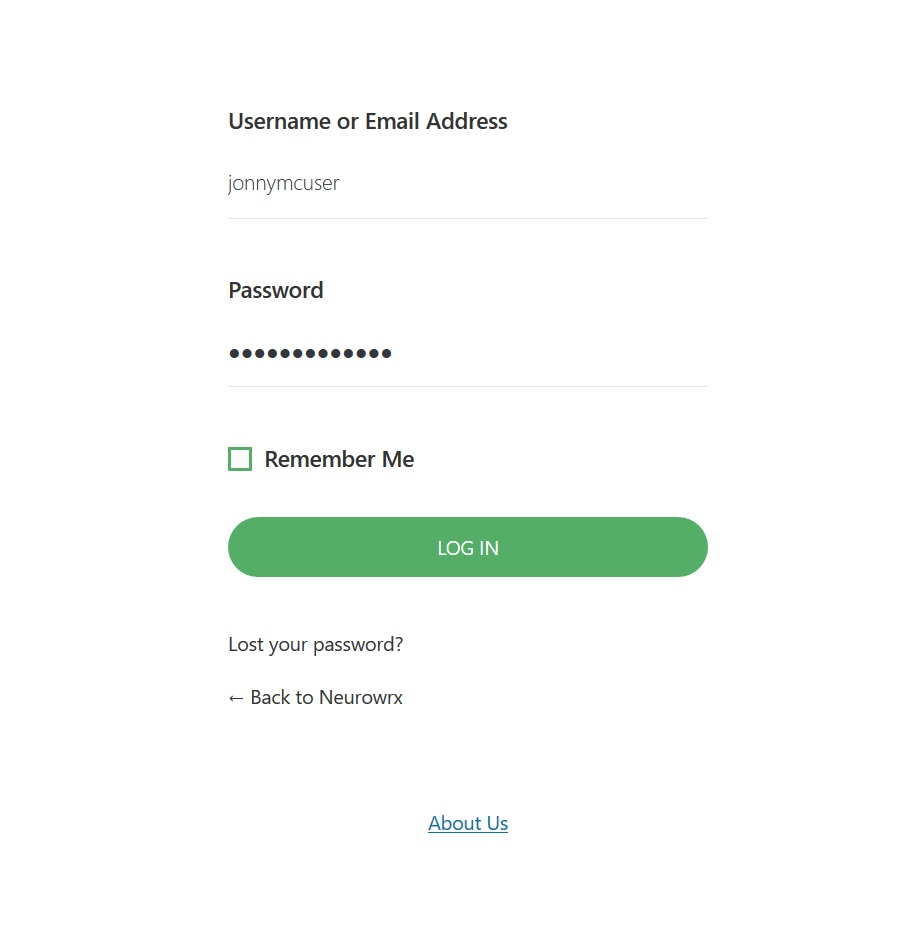
\includegraphics[scale=0.3]{images/loginpage.jpg}
    \caption{The login page}
    \label{loginpage}
\end{figure}

\begin{flushleft}
After you have chosen your password, you can log in with either your username, or with your email address.  Both are required to be unique, and in the case that you have more than one account; you must provide distinct email addresses for distinct accounts. 
\end{flushleft}

\begin{flushleft}
Once a successful login has occurred, the top panel of the website changes to give the user access to the communication features.  A link for the members section appears, as well as an icon for private messages, notifications, and another for settings.  There is also a menu hiding under the profile picture with more features which will be discussed in succeeding sections. 
\end{flushleft}

\begin{figure}[h]
    \centering
    
\includegraphics[scale=0.3]{images/topbar.jpg}
    \caption{The top panel that is publicly visible}
    \label{topbar}
\end{figure}

\begin{figure}[h]
    \centering
    
\includegraphics[scale=0.3]{images/topbarlogged.jpg}
    \caption{The top panel after login}
    \label{topbarlogged}
\end{figure}

\subsection{Activity} \label{Activity}

\begin{flushleft}
A user can perform an action similar to "tweeting".  It consists of creating a small, constrained text block that is associated with their account and will be visible to their followers.  They can also tweet in a particular group.  This is intended for public conversations of a less involved form than forum posts.  
\end{flushleft}

\begin{flushleft}
The activity feed also contains automatically generated messages that let you and other members know what is going on with you account in other ways, such as informing followers if you have been promoted to a moderator, or when you have gained admittance to a group.  To view your activity feed; either click your profile picture in the top right corner, or click on the activity link in the dropdown menu under it. 
\end{flushleft}

\begin{figure}[H]
    \centering
    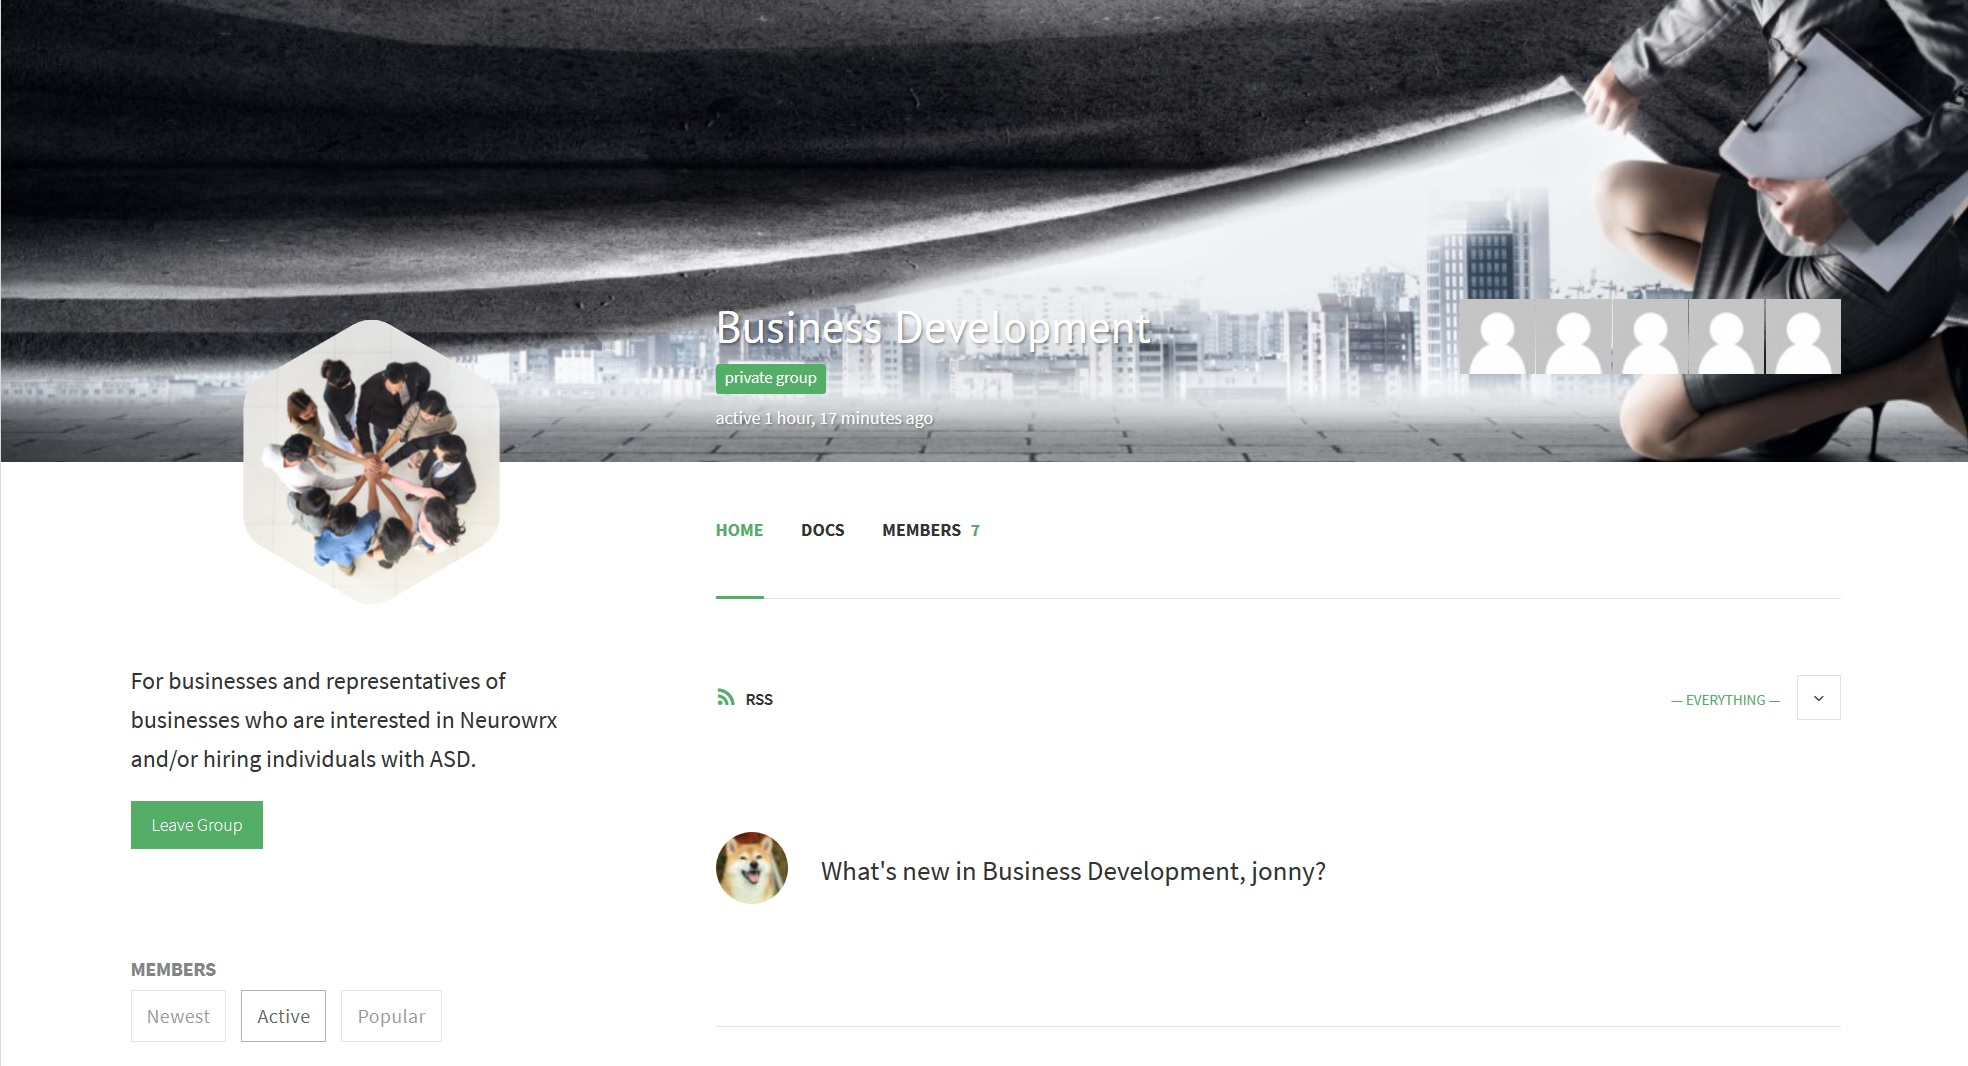
\includegraphics[scale=0.3]{images/whatsnew.jpg}
    \caption{The activity feed associated with a user account}
    \label{whatsnew}
\end{figure}

\begin{flushleft}
To inform your followers of something, move the cursor over the text "What's new, <your first name>?" (see figure \ref{whatsnew}) and left click. This will allow you to enter some text.  Type whatever it is you wish to say and then click "publish" (see figure \ref{bowwow}).  For comments that either you or others have made, there are black buttons on the right that allow the viewer to reply, like, or (given appropriate permissions) delete (from left to right).  A user can always delete their own comments, but only moderators and admins can delete the comments of others.   
\end{flushleft}

\begin{figure}[h]
    \centering
    \subfloat{{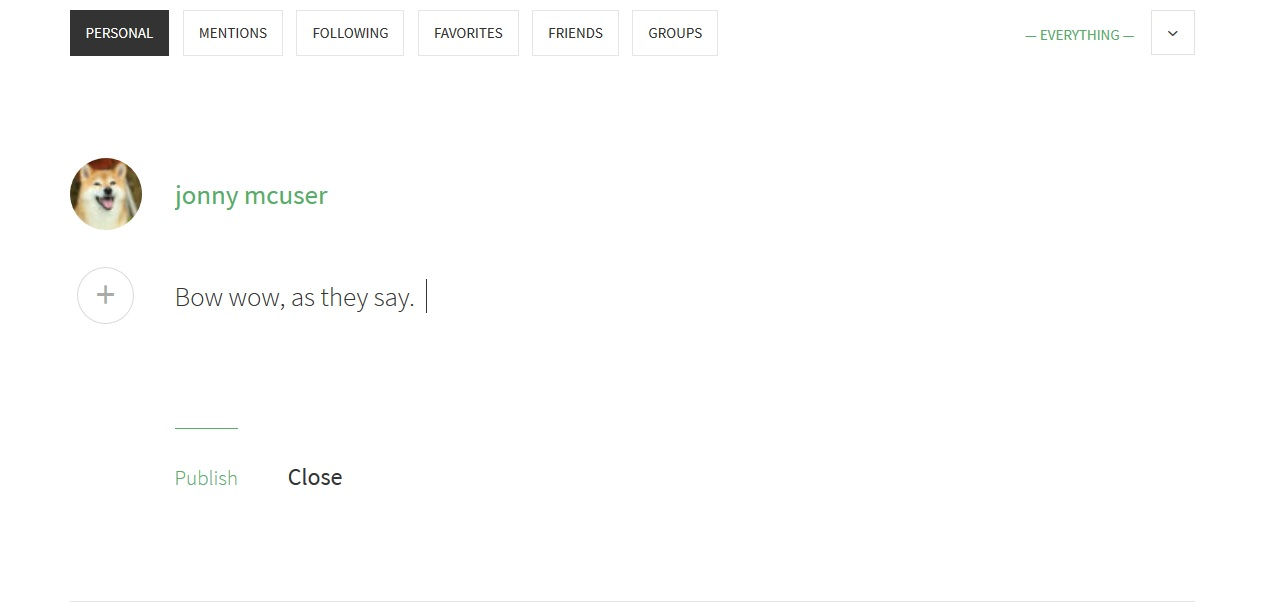
\includegraphics[scale=0.25]{images/bowwow.jpg}}}
    \qquad
    \subfloat{{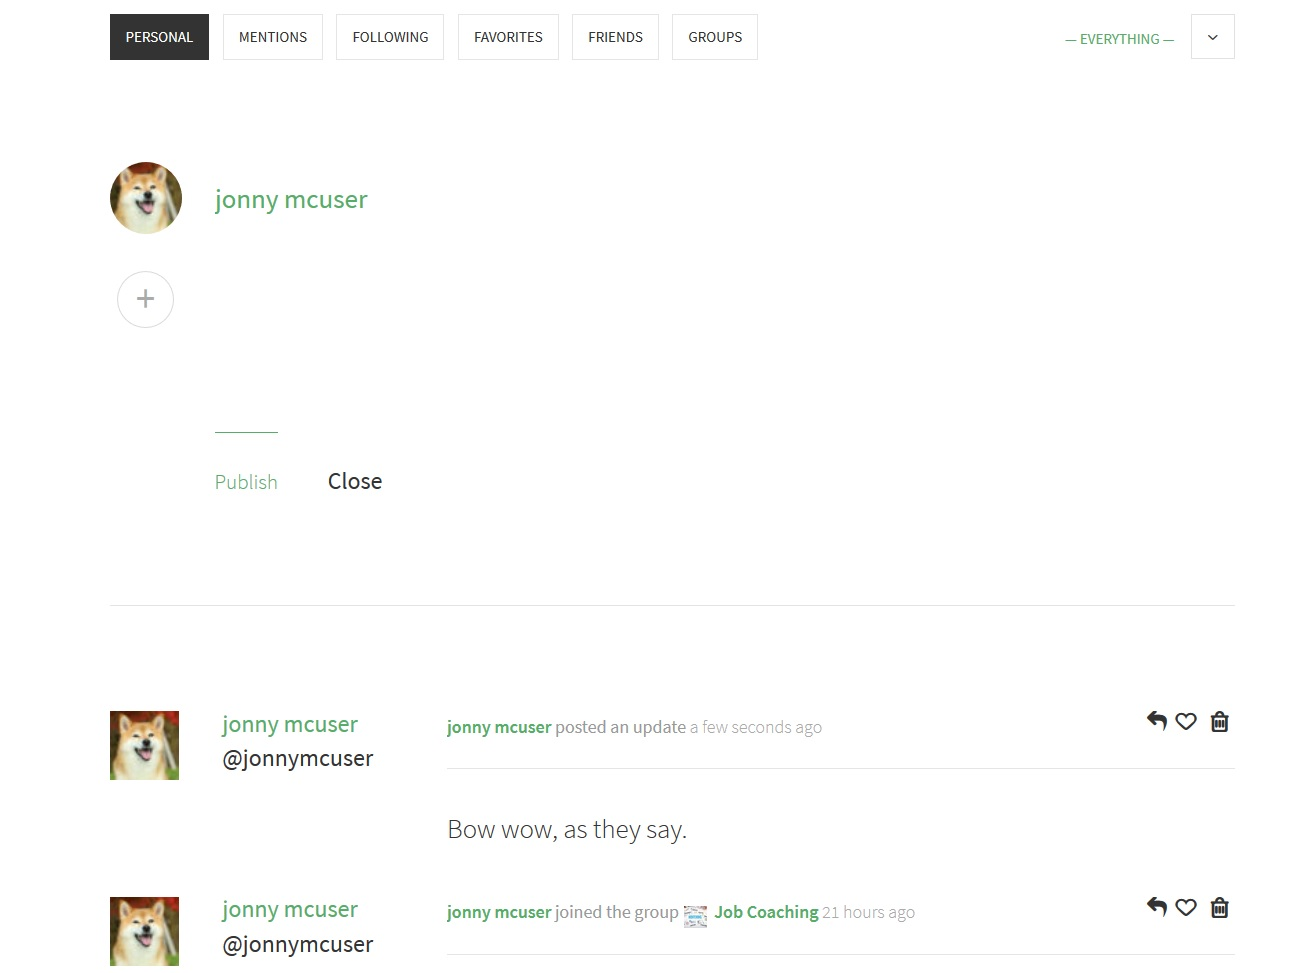
\includegraphics[scale=0.25]{images/bowwowed.jpg}}}
    \caption{An item has been added to your activity feed}
    \label{bowwow}
\end{figure}

\begin{flushleft}
Another feature that bears mentioning is the "+" button to the left of the text in the above mentioned menu.  If you click on it, a small play icon appears (see figure \ref{linkpost}).
\end{flushleft}

\begin{figure}[H]
    \centering
    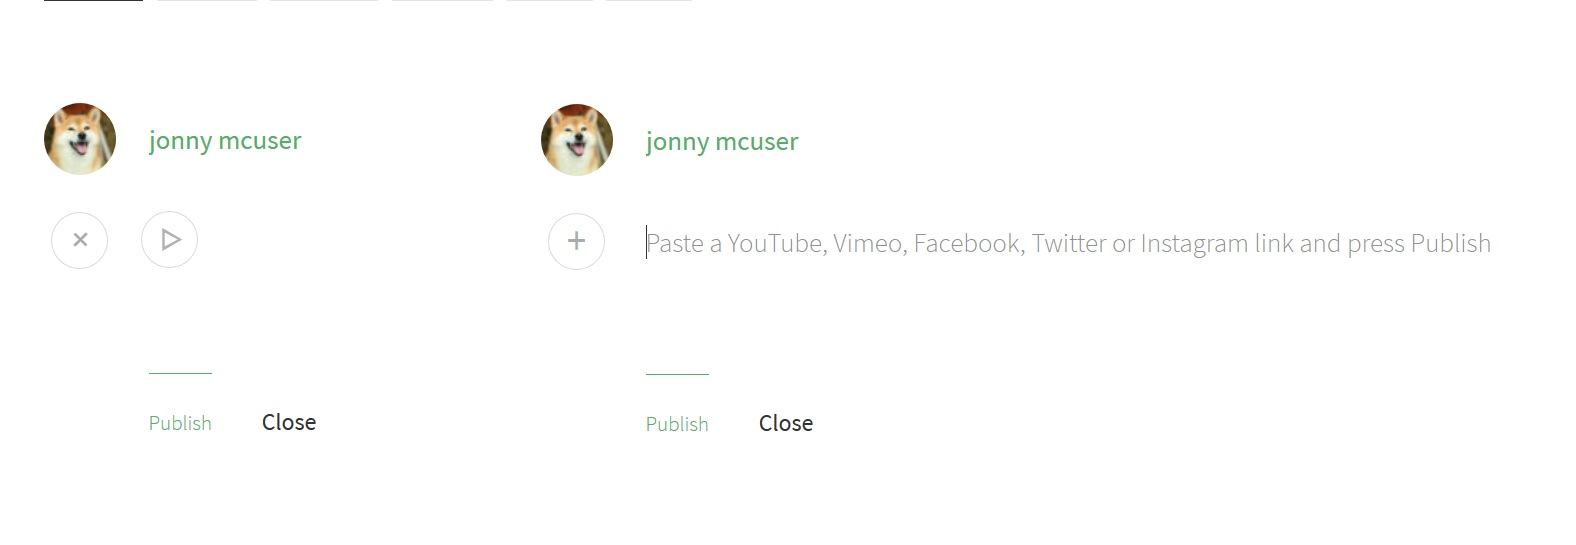
\includegraphics[scale=0.3]{images/linkpost.jpg}
    \caption{The post link button}
    \label{linkpost}
\end{figure}

\begin{flushleft}

At this point, one can post a link to a youtube video (or one of the other kinds of content listed) and publish.  In all cases, what is expected is the url of the content.  For example, this is what result of posting the url "https://www.youtube.com/watch?v=ajHWBMhfxnM" using the posting feature (figure \ref{videopost}).

\end{flushleft}

\begin{figure}[H]
    \centering
    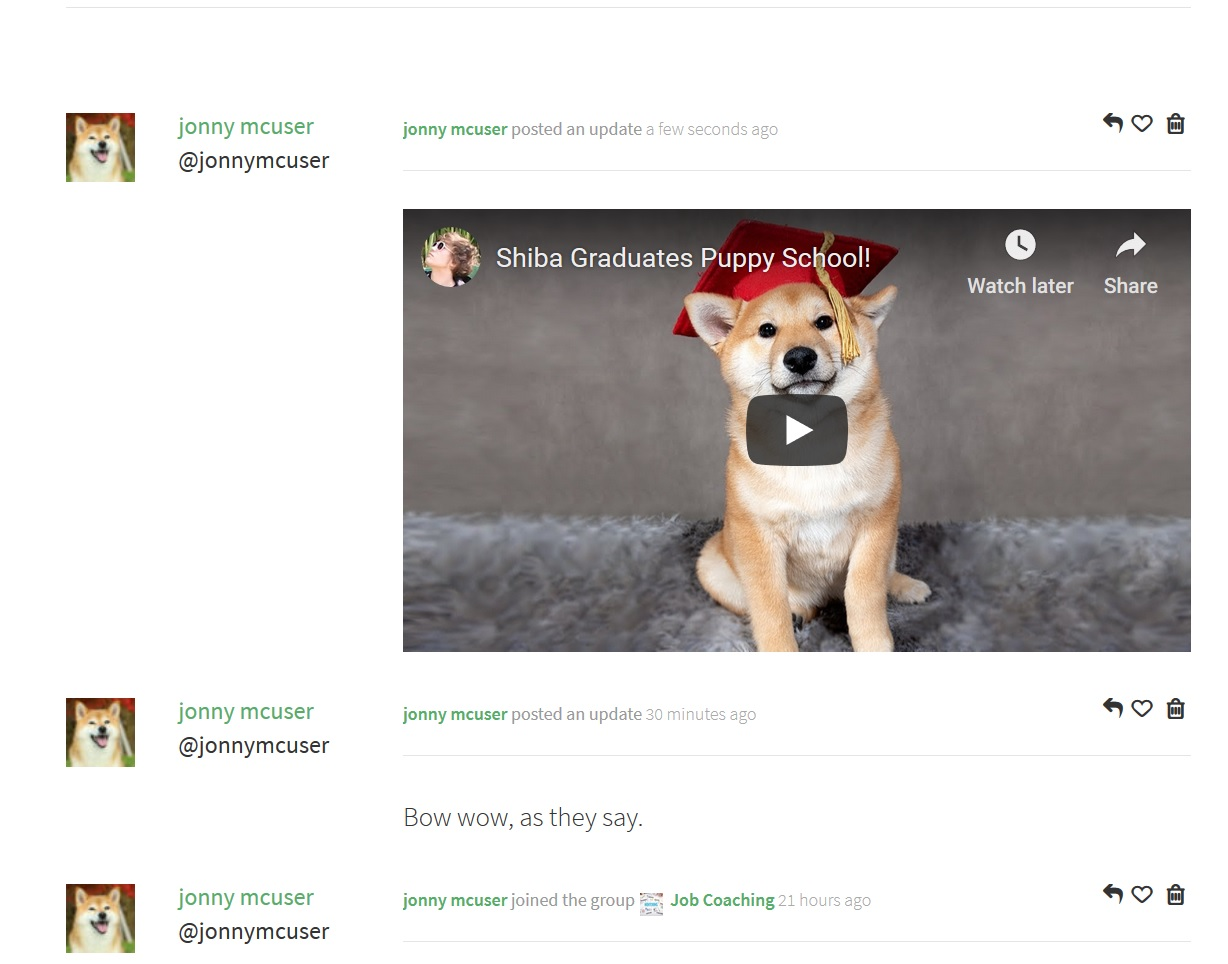
\includegraphics[scale=0.3]{images/puppyschool.jpg}
    \caption{Posting a youtube video}
    \label{videopost}
\end{figure}

\begin{flushleft}
The purpose of this feature is to save people the trouble of having to follow the link to see what the video is about (in case they don't care, let's say), and also to avoid having to host the video on the neurowrx website (which would be wasteful).  Instead, the video is still on youtube (in this case), but the thumbnail and title is visible in the post.  
\end{flushleft}

\begin{flushleft}
The other sections of the activity page are for different categories of activity that one can choose to view and respond to (see figure \ref{whatsnew}).  For an ordinary user, these are: Personal, which are either made by you or auto-generated by you account (this is the one you can add to manually, as discussed above), Mentions, which contains activity that mentions you in some way, Following, which is an aggregator for activity of people that you have chosen to follow, Favourites, which keeps track of content you have favourited (kind of like following, but for topics instead of people), Friends, the people on your friendslist, and Groups, the activity in the groups that you are a part of.  
\end{flushleft}

\begin{flushleft}
There is also a dropdown menu on the right for filtering content further, according to certain tags.  By default it just shows everything in a particular category.  
\end{flushleft}


\subsection{Your Neurowrx profile}

\begin{flushleft}
By hovering the mouse over the profile pic, a dropdown menu (with association submenus) becomes available.  The profile functions can either be accessed though the profile submenu or by clicking on "profile" itself to go to the profile page.  
\end{flushleft}

\begin{figure}[H]
    \centering
    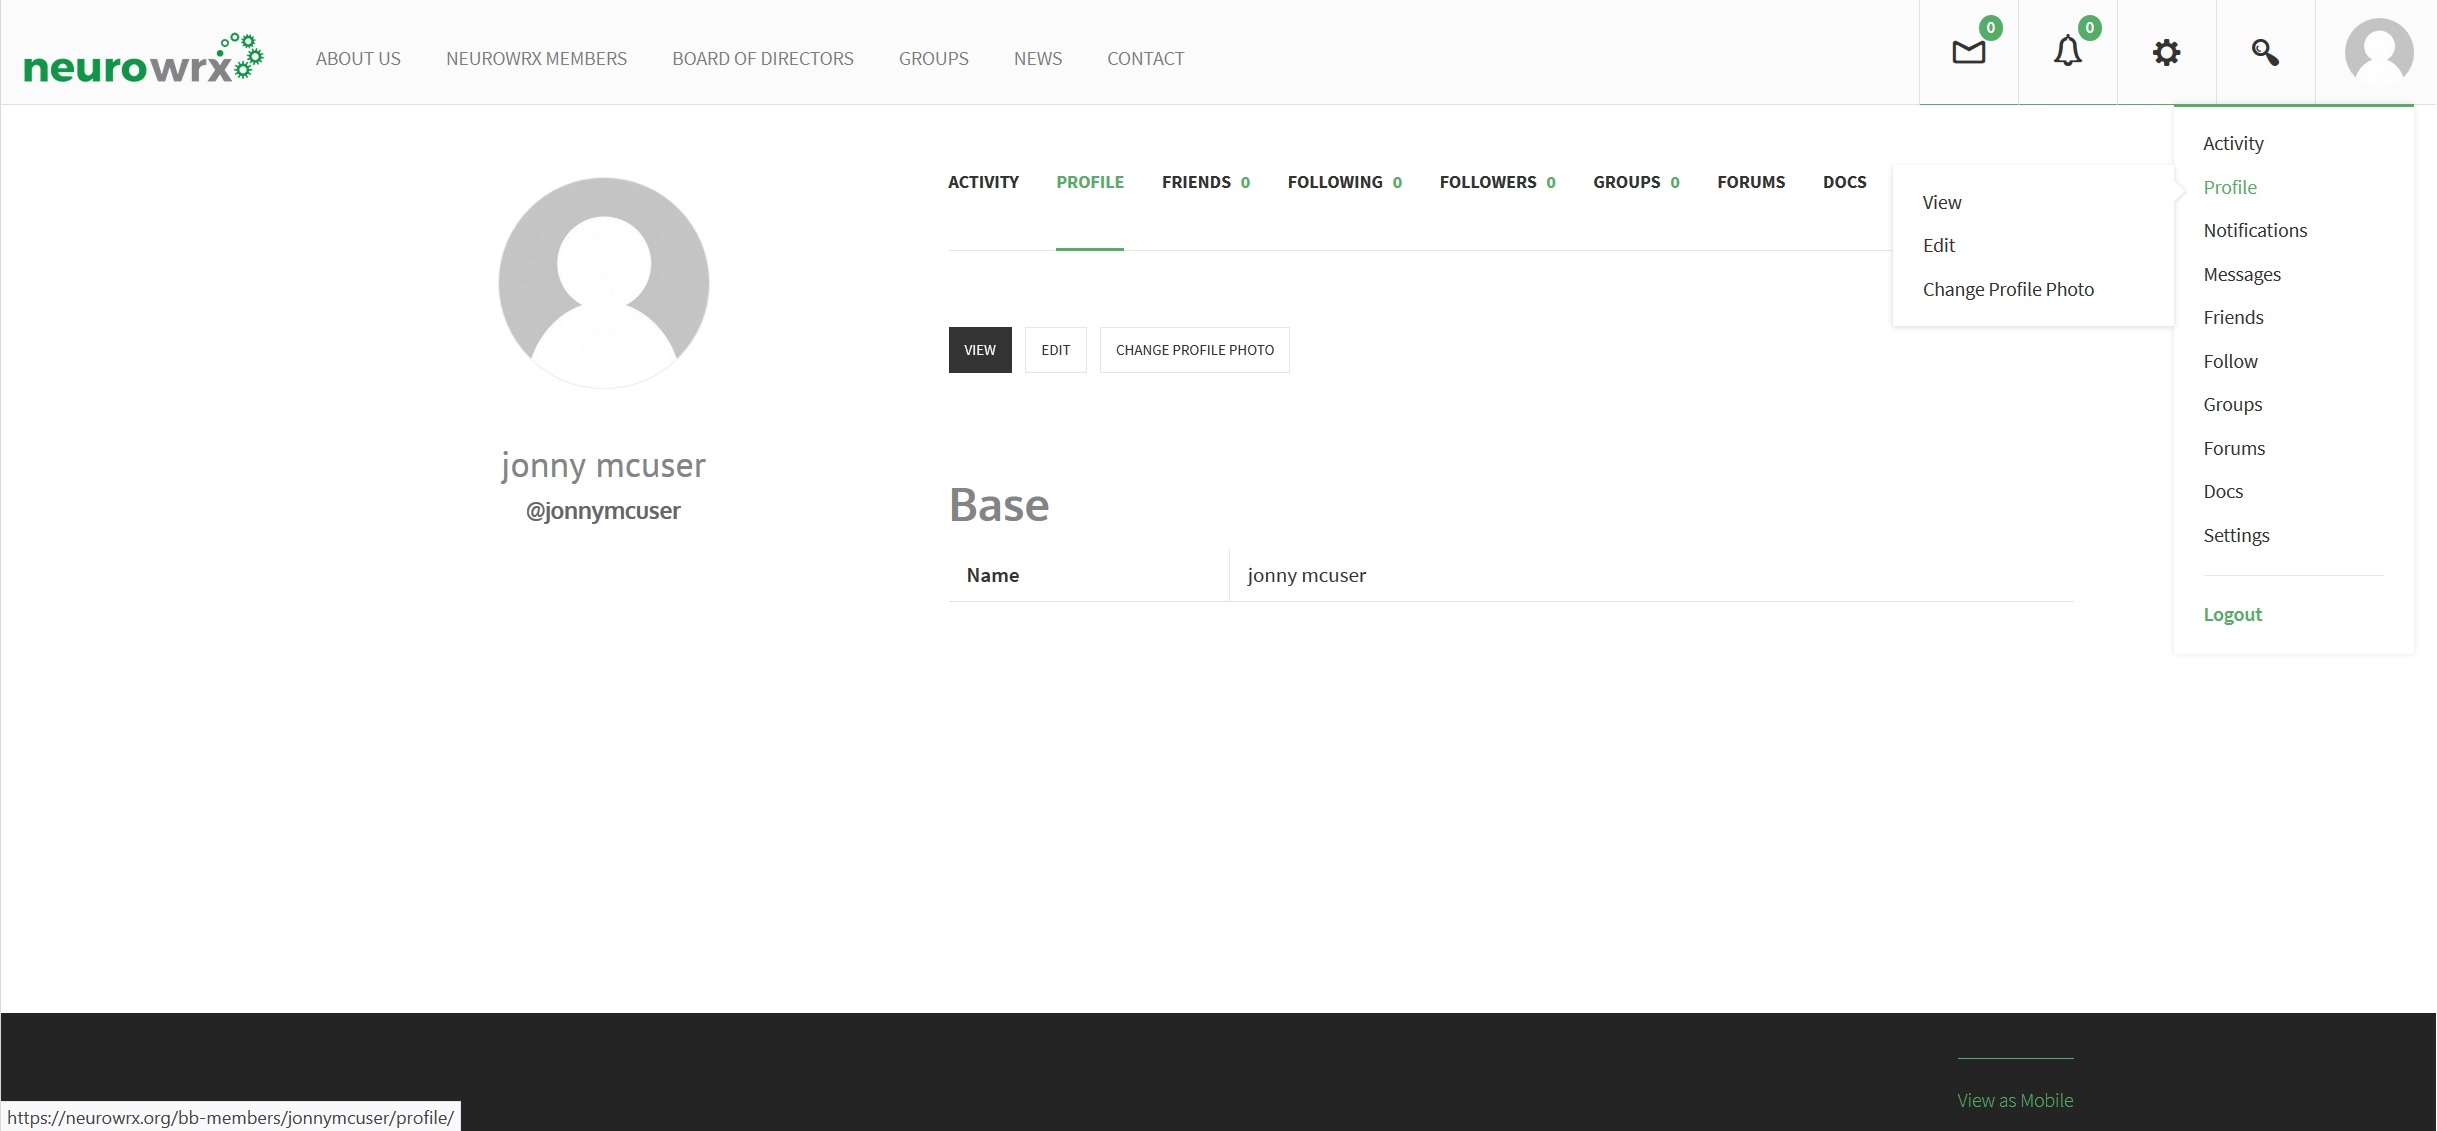
\includegraphics[scale=0.2]{images/profile.jpg}
    \caption{The profile page, and the profile menu that can be used to navigate to it.}
    \label{profilepage}
\end{figure}

\subsubsection{Changing your profile picture}

\begin{flushleft}
When you add a profile picture (which is optional), you can either upload an existing file by dragging the file into the hatched boundary box (which doesn't work on all operating systems), open a file selection window by clicking the green button, or click the "Take Photo" link to activate your webcam (assuming that you have one plugged in).  This step makes the an image file available to the cropping tool, which you will use to select a small square shaped section of the image (presumably your face) for use as your face on the forums and in the messaging system. 

\end{flushleft}
 The image is required to be of the .jpeg, .gif, or .png file formats.  It is also recommended that you use an image that is of at least 280x280 pixels, but this isn't strictly necessary. 
\begin{flushleft}

\end{flushleft}

\begin{figure}[h]
    \centering
    \subfloat{{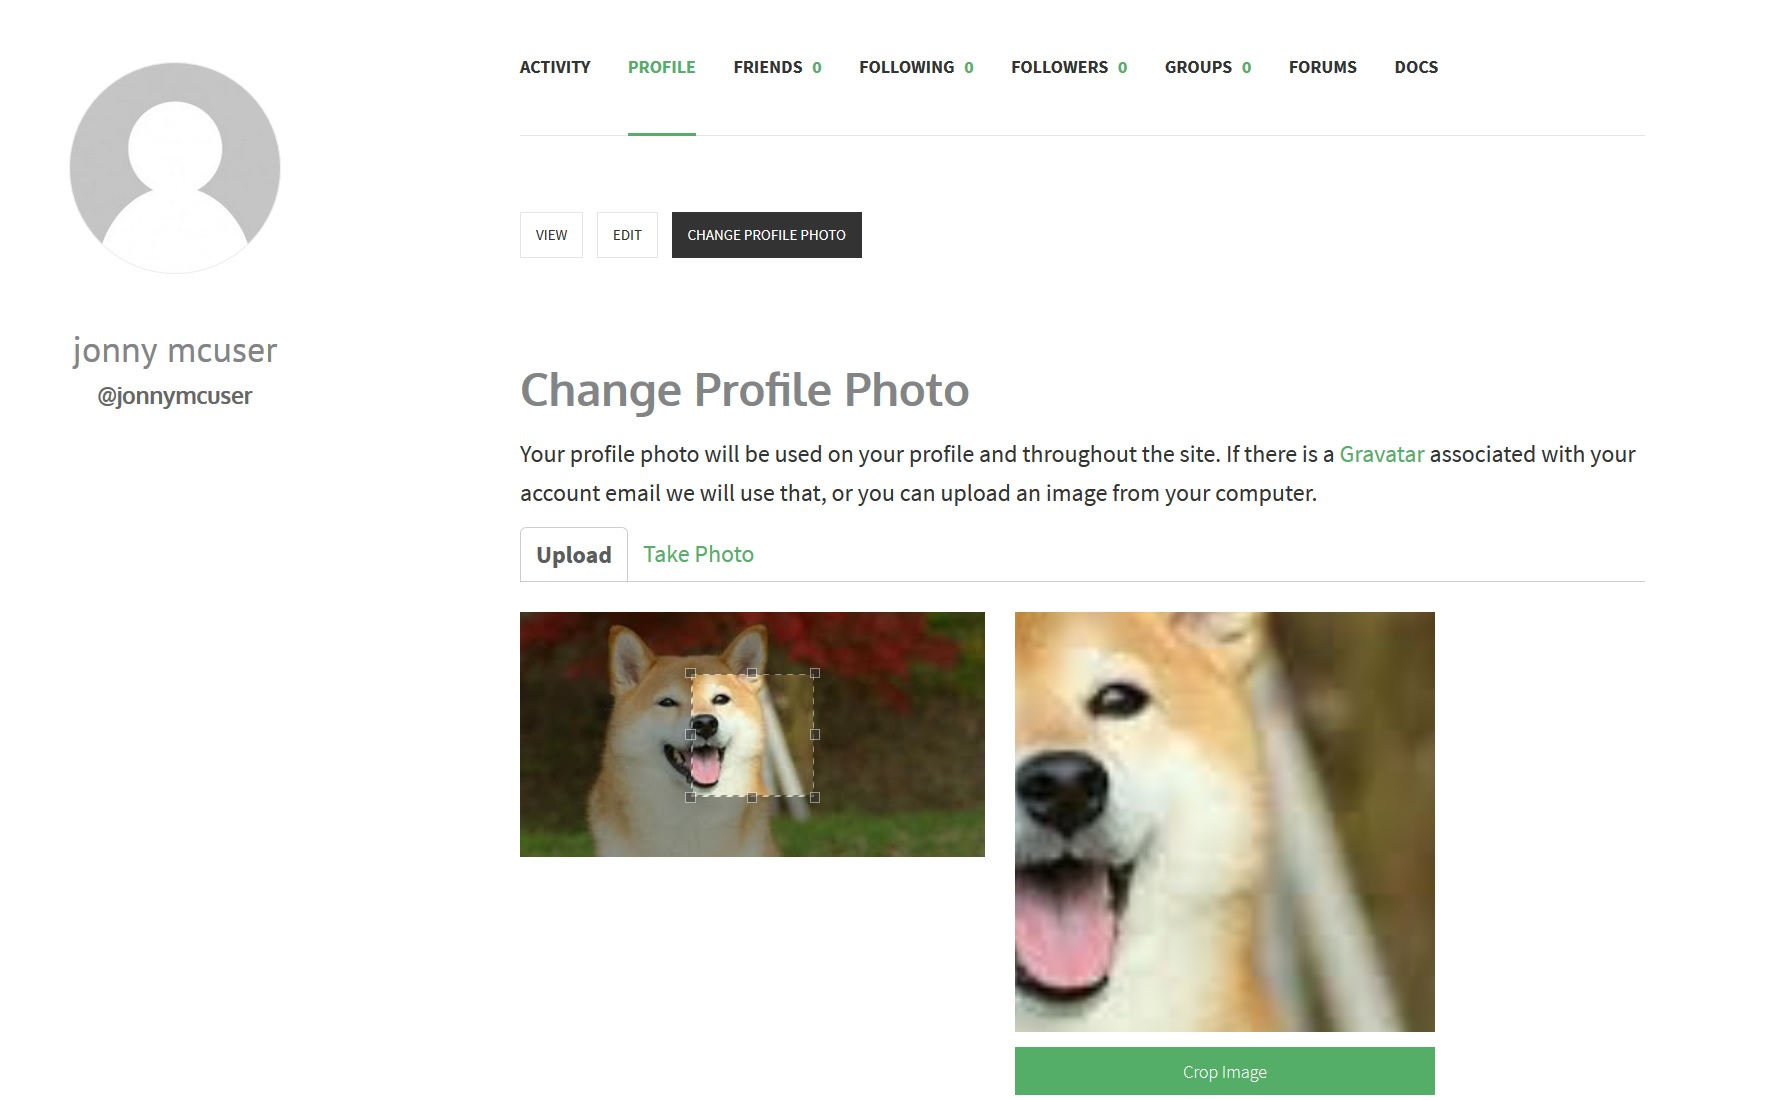
\includegraphics[scale=0.2]{images/doggy.jpg}}}
    \qquad
    \subfloat{{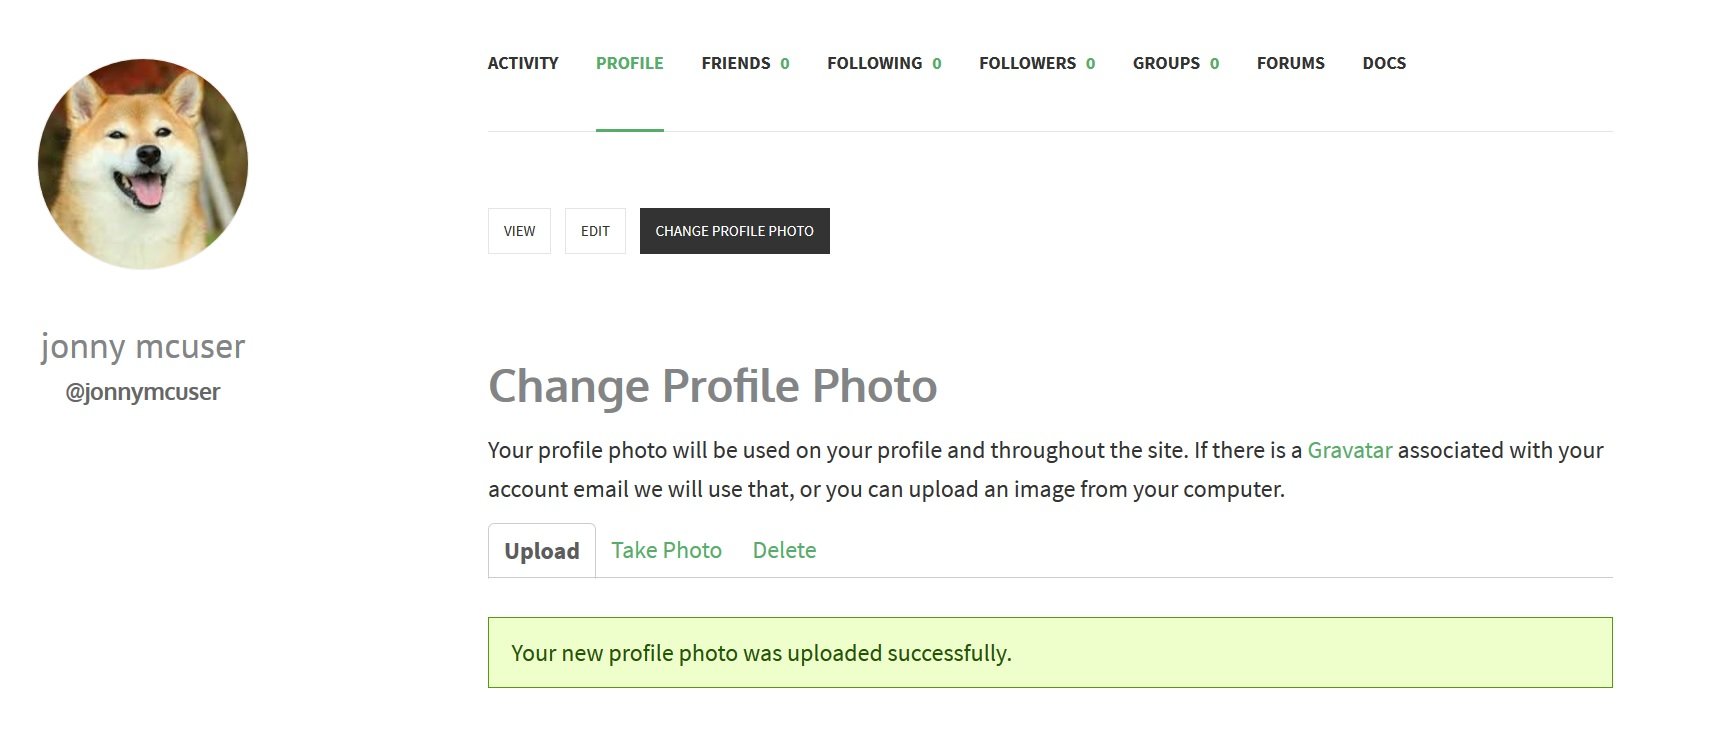
\includegraphics[scale=0.2]{images/doggy2.jpg}}}
    \caption{A successful profile picture upload}
    \label{avatarUp}
\end{figure}

\subsubsection{Editing your other profile information}

\begin{flushleft}
Other than the photo, your Neurowrx profile contains a changeable public Name field (which is not the same as your username) a gender field (which by default has neither selected, and does not have to be chosen) and several fields that you can paste links to your profiles on other social networking services.  At the time of this writing, we have fields for facebook, twitter and a few others.  This list could potentially grow in the future.  
\end{flushleft}

\begin{flushleft}
One is only expected to post the url of the profile in question, the form of which varies from service to service.  If you are unsure what the url to your profile is, consult the documentation for that particular service. 
\end{flushleft}

\subsection{Notifications} \label{Notifications}
\begin{flushleft}
The next section of the dropdown menu is the notifications aggregator. This can be accessed from the dropdown menu beneath the profile link, or by clicking the bell icon on the top panel.  It's purpose is to inform the user of events inside the bureaucracy of the website that pertain to them.  These include friendship requests, group admissions, promotions or demotions, etc.   
\end{flushleft}

\begin{figure}[H]
    \centering
    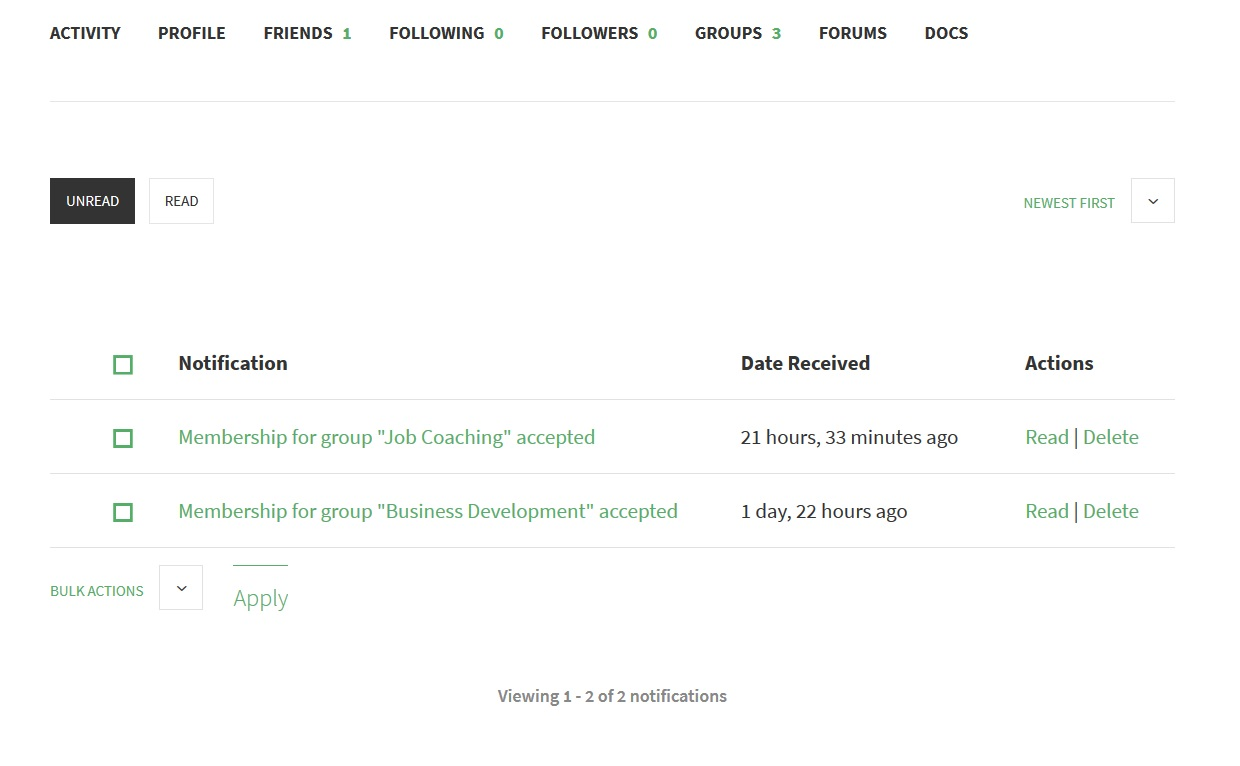
\includegraphics[scale=0.5]{images/notifications.jpg}
    \caption{The notifications page.}
    \label{notifpage}
\end{figure}

\begin{flushleft}
As can be seen in figure \ref{notifpage}, each notification can be read or deleted.  If you wish to mark several notifications as read or deleted at once, select all that you wish to apply the bulk action to via the checkboxes on the left.  The click the bulk actions drowndown menu and select either "mark read" or "delete".  Then click apply to perform the action. 
\end{flushleft}

\begin{flushleft}
The bell on the top panel has an orange number on it that denotes the number of unread notifications. 
\end{flushleft}

\subsection{Messages}

\begin{flushleft}

The next section of the dropdown menu is the messaging page.  It can be accessed from the dropdown menu beneath the notifications link, or by clicking the envelope icon on the top panel.  It's purpose is to allow the user to send messages directly to other users, privately.  It works much the same way as email, where usernames take the place of email addresses.


\end{flushleft}

\begin{figure}[H]
    \centering
    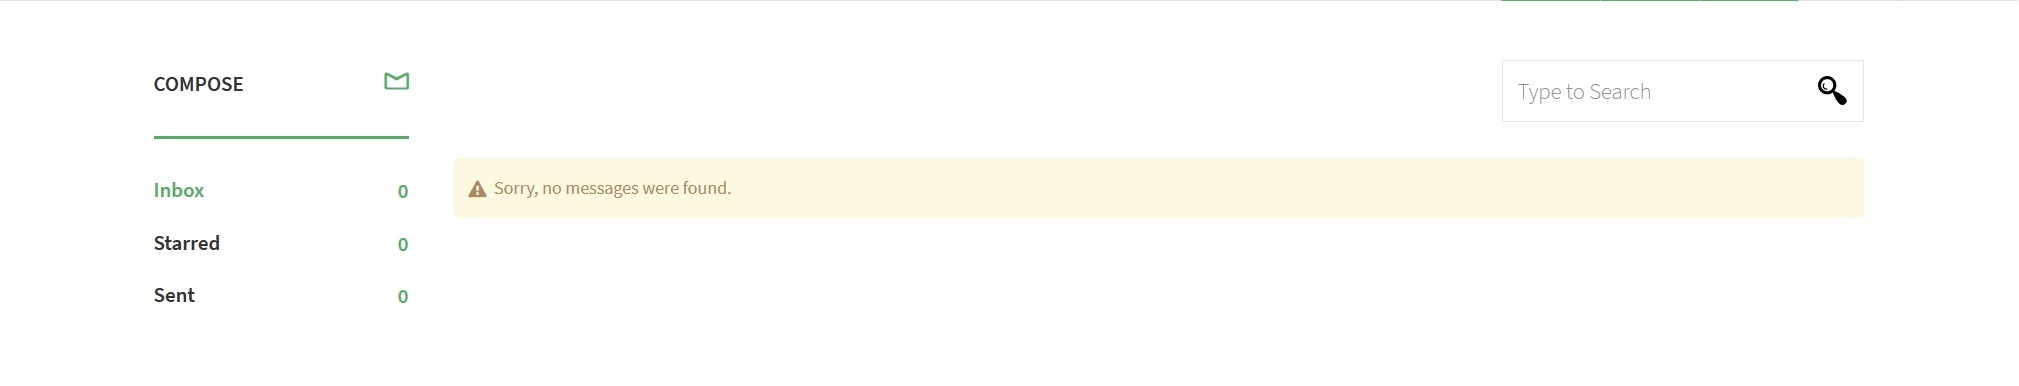
\includegraphics[scale=0.5]{images/messaging.jpg}
    \caption{The messaging page}
    \label{messaging}
\end{figure}

\begin{flushleft}

In the default view (see figure \ref{messaging}), the contents of the inbox are displayed.  From here one could click on a message to display it, after which point it would be marked as read.  The current number of unread messages in the inbox is always visible by the green number in the corner of the envelope icon on the top panel.  It is also visible to the right of the word "inbox" on the messaging page. 

\end{flushleft}

\begin{flushleft}
The send a message, click the compose link to the left of the green envelope.  You are presented with three fields (see figure \ref{sos}).  Send To, Subject, and Message.  When you begin to type a username or name into the Sent To field, it suggests autocompletes from your friends list (see section \ref{Friends}).
\end{flushleft}

\begin{figure}[H]
    \centering
    \subfloat{{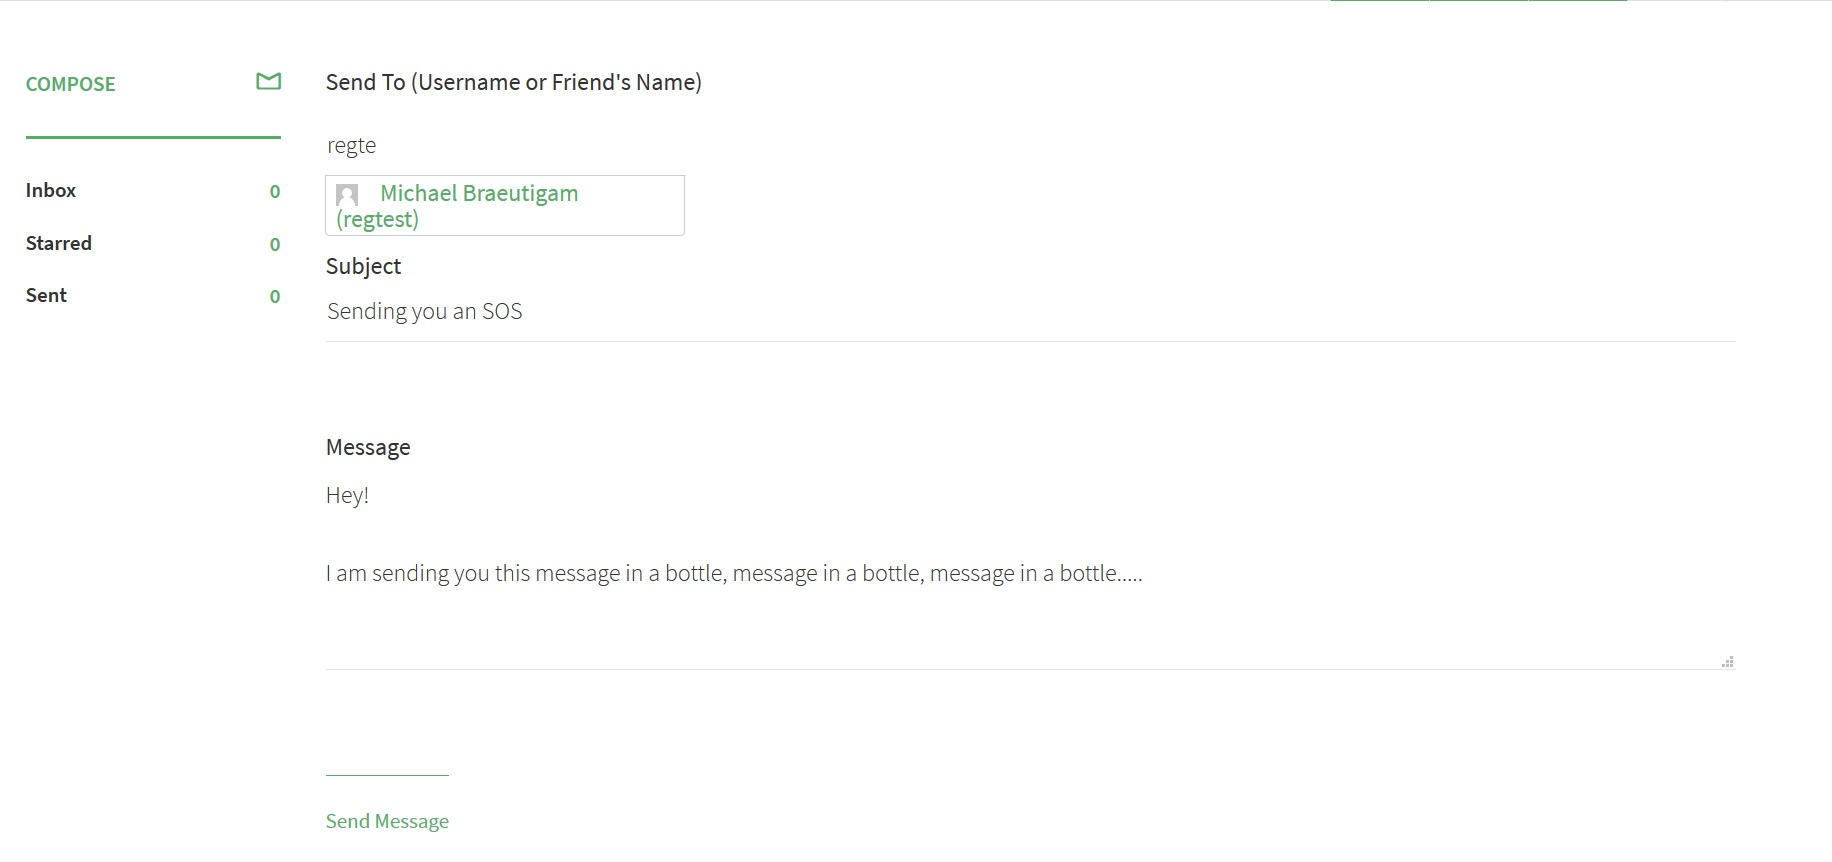
\includegraphics[scale=0.23]{images/sos.jpg}}}
    \qquad
    \subfloat{{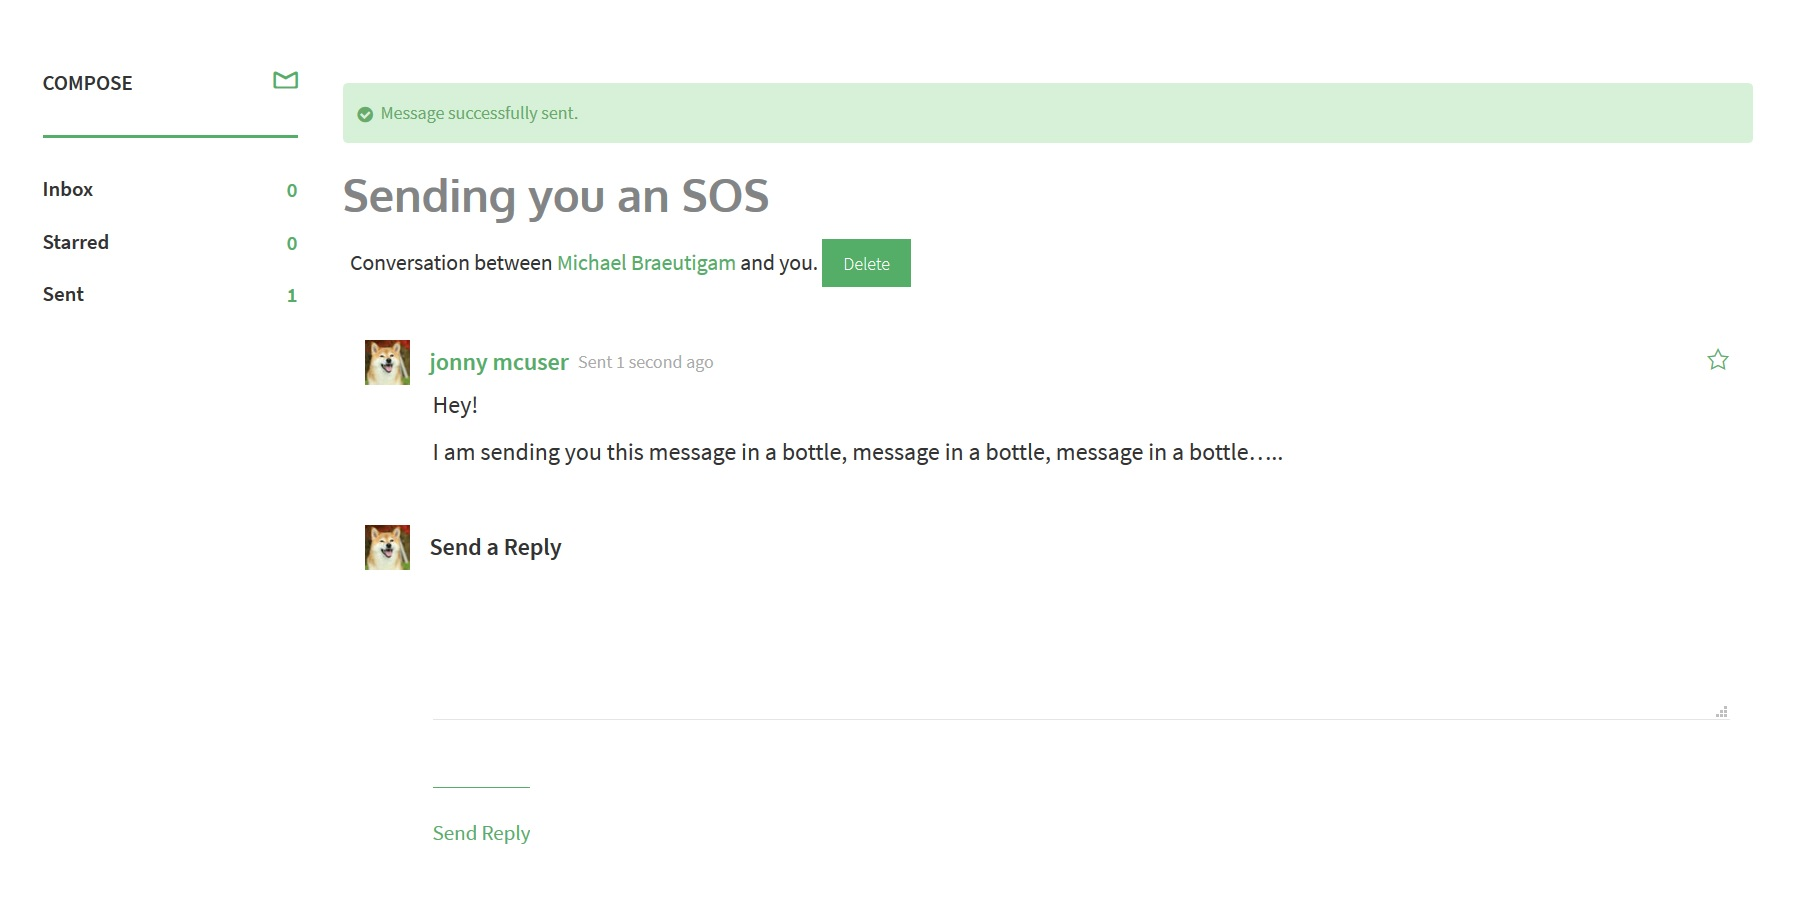
\includegraphics[scale=0.23]{images/sossent.jpg}}}
    \caption{The sending of a message}
    \label{sos}
\end{figure}

\begin{flushleft}
You will notice an empty star to the right of the sent message in the right half of figure \ref{sos}.  If this is clicked, the conversation in question is regarded as being relatively important, and it is moved to the "starred" category which can be viewed by clicking the link on the left.  Right by this, there are also links to change the read/unread status as well as delete the message. 
\end{flushleft}

\subsection{Friends}  \label{Friends}

\begin{flushleft}
In the dropdown menu, under the profile pic, beneath the messaging link, there is a link to the friendships page.  There is also a link to this page called "friends" at the top of the users personal page, just to the right of the profile link.  
\end{flushleft}

\begin{flushleft}
The primary utility of having people in your friends list is that when you send them messages the site provides autocomplete suggestions of the name as you are typing it in, so if the person in question is someone you communicate with fairly often it is convenient. Their activity also makes it onto your activity feed.
\end{flushleft}

\subsubsection{Adding and Removing Friends}

\begin{flushleft}
To add someone to your friends list, you must first see their profile picture somewhere on the site so that you can click on it.  In all likelihood, this will be throught a group that you are both a member of, or it could perhaps be though a conversation on someones activity feed.  Regardless, all profile pictures are clickable links to the users page (see figure \ref{profilelink})
\end{flushleft}

\begin{figure}[H]
    \centering
    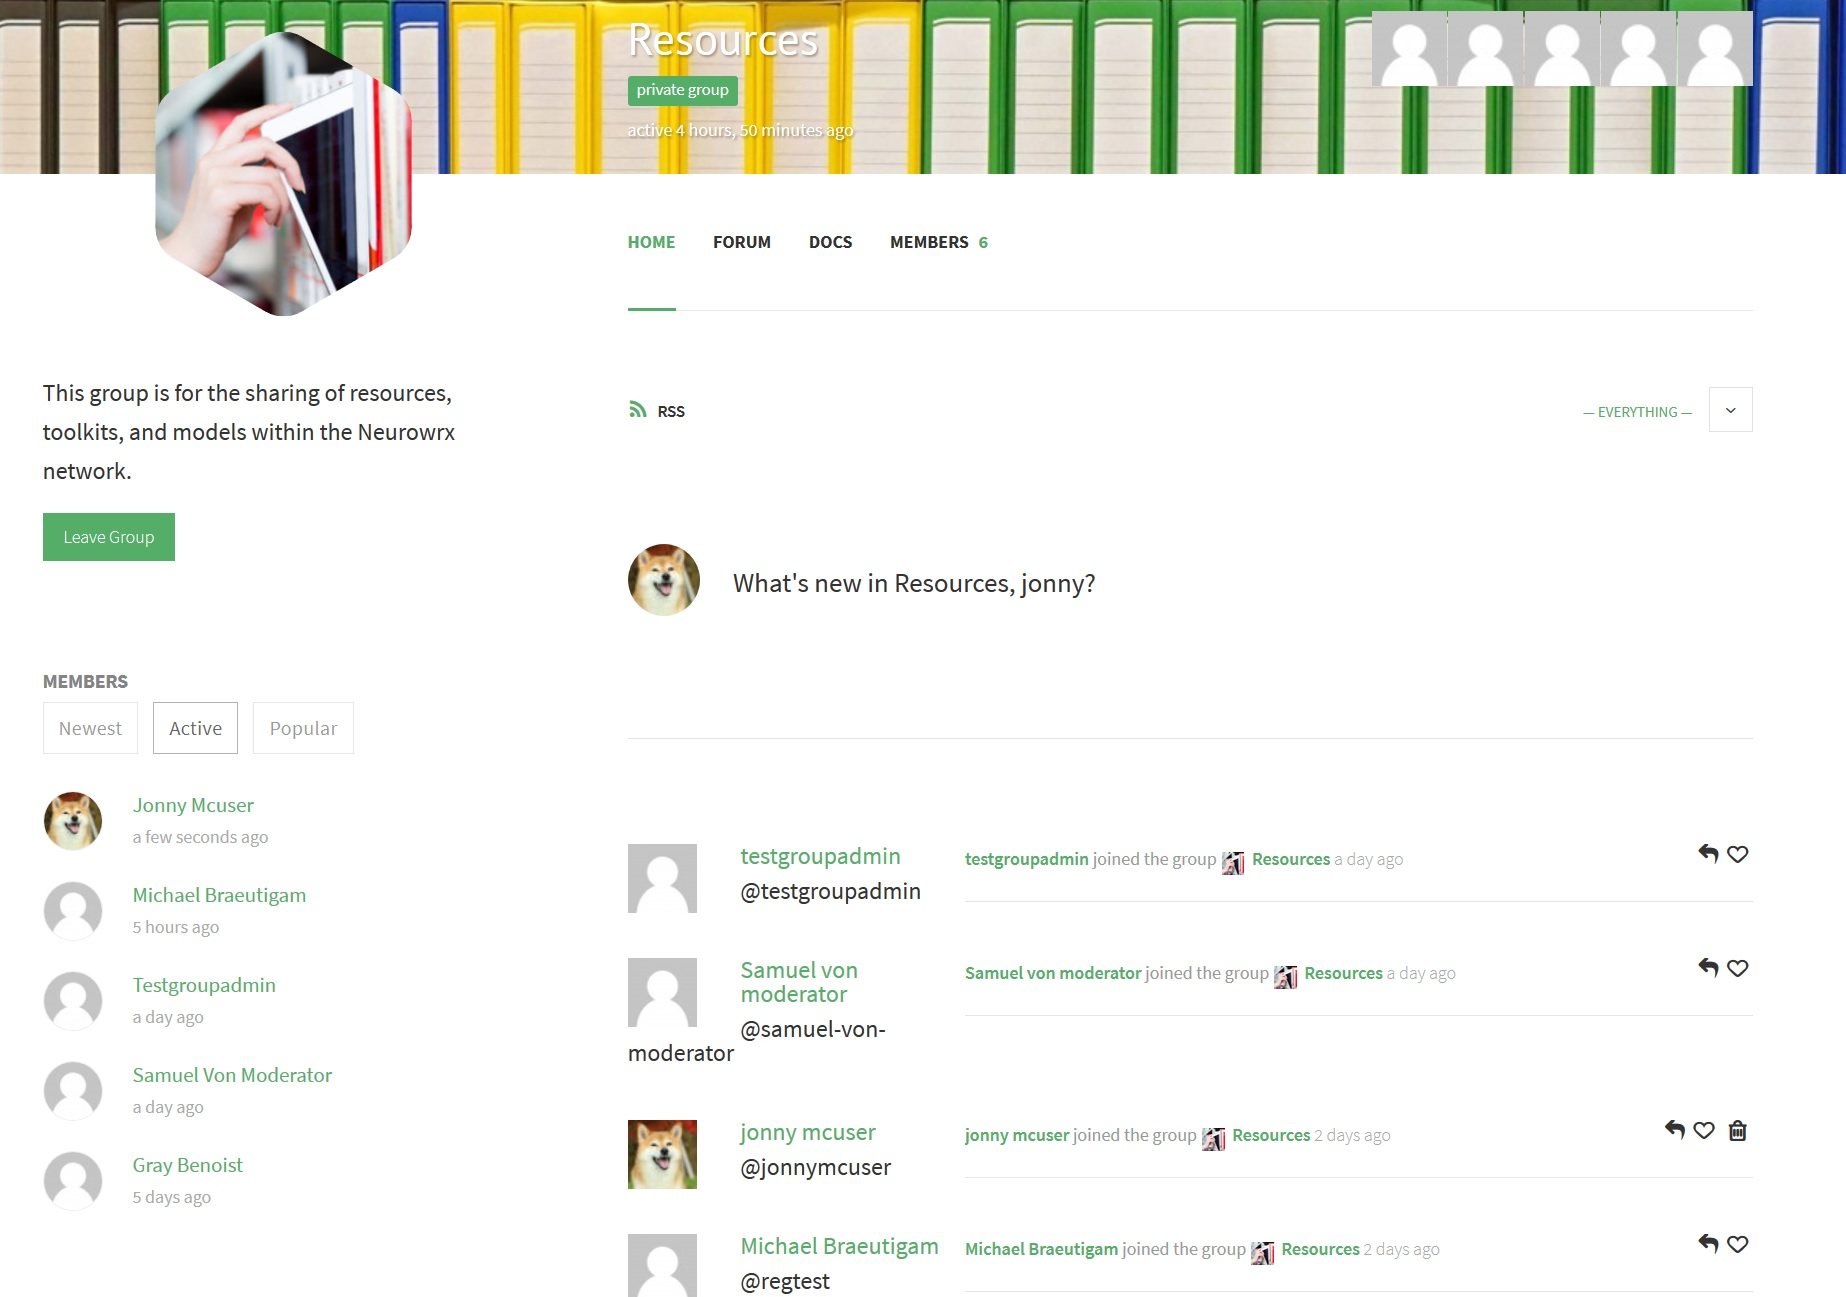
\includegraphics[scale=0.3]{images/resources.jpg}
    \caption{A group page, note the members list on the left.  Those names and pictures are links to the associated user pages.}
    \label{profilelink}
\end{figure}

\begin{flushleft}

On a particular users page, it is apparent when looking at their profile picture whether or not they are already a friend (see figure \ref{friendyesno}).  If you wish to add a friend, click the respective button and a request will be sent to them.  If they accept, you will receive a notification (see section \ref{Notifications}).

\end{flushleft}

\begin{figure}[H]
    \centering
    \subfloat{{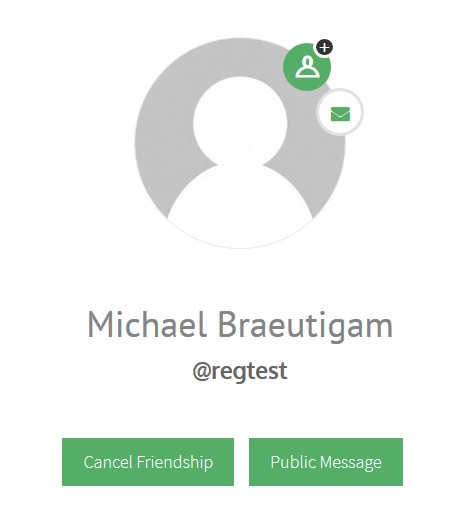
\includegraphics[scale=0.23]{images/friend.jpg}}}
    \qquad
    \subfloat{{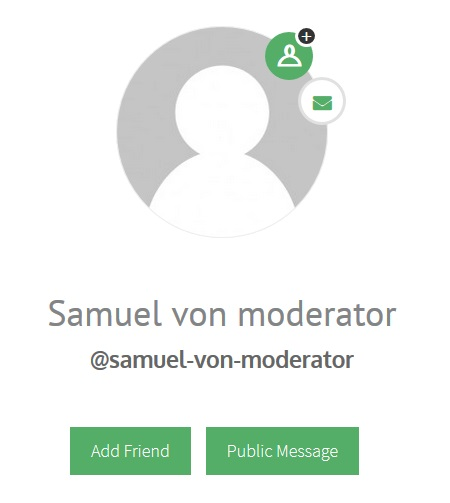
\includegraphics[scale=0.23]{images/notfriend.jpg}}}
    \caption{A friend and someone who isn't (yet)}
    \label{friendyesno}
\end{figure}

\begin{flushleft}
You can also cancel a friendship by the same method, although this does not require their approval, nor give them notification.
\end{flushleft}

\subsubsection{Accepting Friends}
\begin{flushleft}
The process for accepting someone else's friend request is slightly different.  When you receive a friend request, a notification shows up on your notifications page and your bell icon (see section \ref{Notifications}).  You could go directly to the friend request page by clicking this notification (see figure \ref{request})
\end{flushleft}


\begin{figure}[h]
    \centering
    \subfloat{{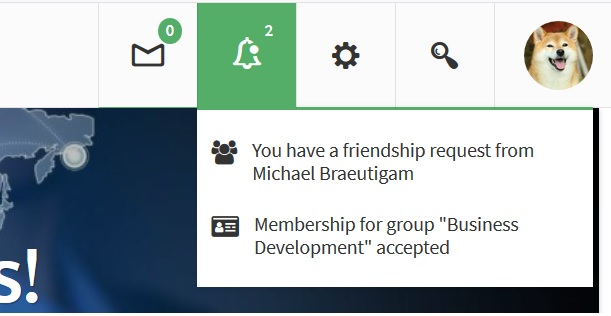
\includegraphics[scale=0.35]{images/friendreq.jpg}}}
    \qquad
    \subfloat{{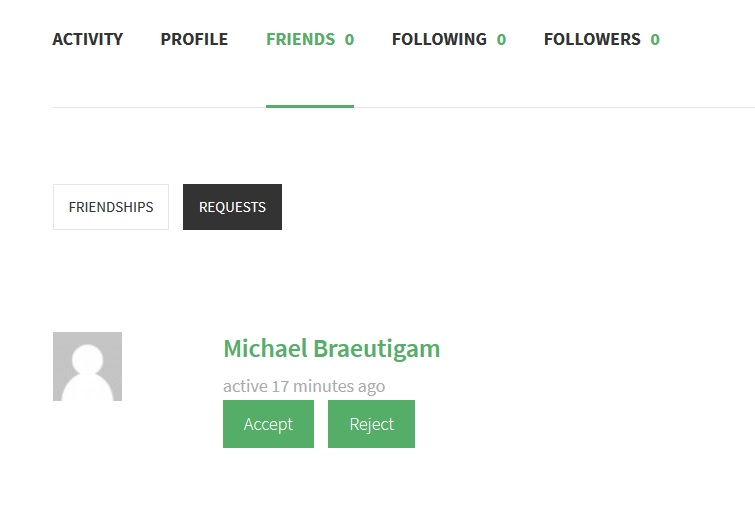
\includegraphics[scale=0.40]{images/requestyesno.jpg}}}
    \caption{The notification associated with a friend request (left), and the request itself (right) awaiting a response}
    \label{request}
\end{figure}

\begin{flushleft}
As one can see in the image on the above right, one can also view pending friend requests by going to the frinds page, and clicking the "requests" button. 
\end{flushleft}


\subsection{Followers}
\begin{flushleft}
Following someone adds their actions to your activity feed (see section \ref{Activity}). The followers function is very similar to the friends function.  One difference is that the relationship is asymmetric (if you follow someone else, it does not ential that they follow you).  Another is that it does not require the approval of the followed.  A third is that people that you are following are not added to the autocompletion list for you message recipients.  
\end{flushleft}


\begin{flushleft}
To follow another user, one simply has to click the follow button next to their profile picture.  It has two appearances depending on where the profile picture is encountered on the site.  The first is is a circle with three horozontal lines across it, located in the lower right.  The second is a green circle with a silhouette of a person with a plus sign in the upper right.   
\end{flushleft}

\begin{figure}[h]
    \centering
    \subfloat{{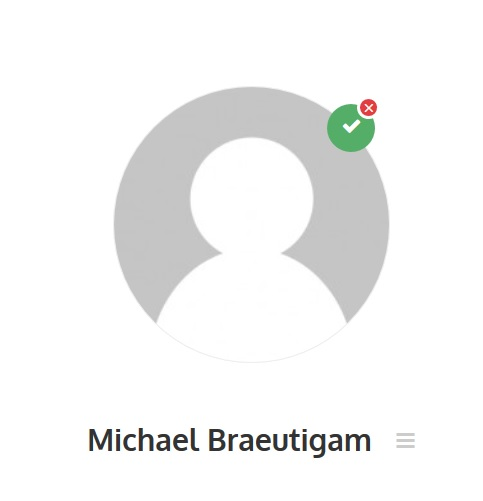
\includegraphics[scale=0.40]{images/userprofilepic.jpg}}}
    \qquad
    \subfloat{{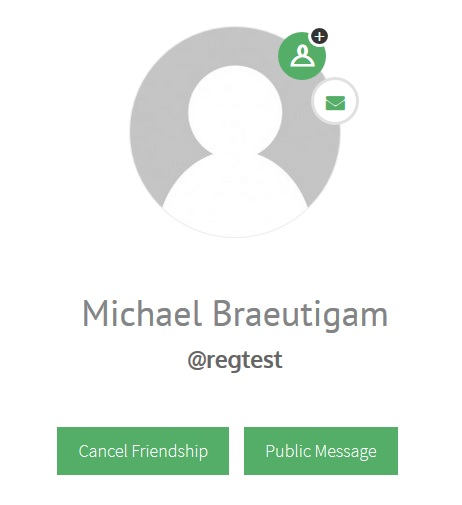
\includegraphics[scale=0.40]{images/userprofilepic2.jpg}}}
    \caption{The two forms of the user profile pic}
    \label{profilepics}
\end{figure}

\begin{flushleft}
To unfollow someone, just reclick the follow button.  
\end{flushleft}

\subsection{Groups}



\begin{flushleft}
Most of the activity on this website occurs within the many groups that members can be part of.  They provide a forum for discussing relevant subject and sharing and editing documents.  There are two main pages where someone can interact with the group functions.  One can be reached by clicking on the "Groups" link located between the board of directors and news links on the top panel of the site.  This page lists all the groups on the site, and is where you request memberships to groups that you are not already a member of.
\end{flushleft}

\begin{flushleft}
The other is located in the menu that arises from hovering the mouse over your profile picture. This section only lists groups that you are currently a member of.  It is also where you can accept invitations to groups that have been extended to you.
\end{flushleft}

\begin{figure}[h]
    \centering
    \subfloat{{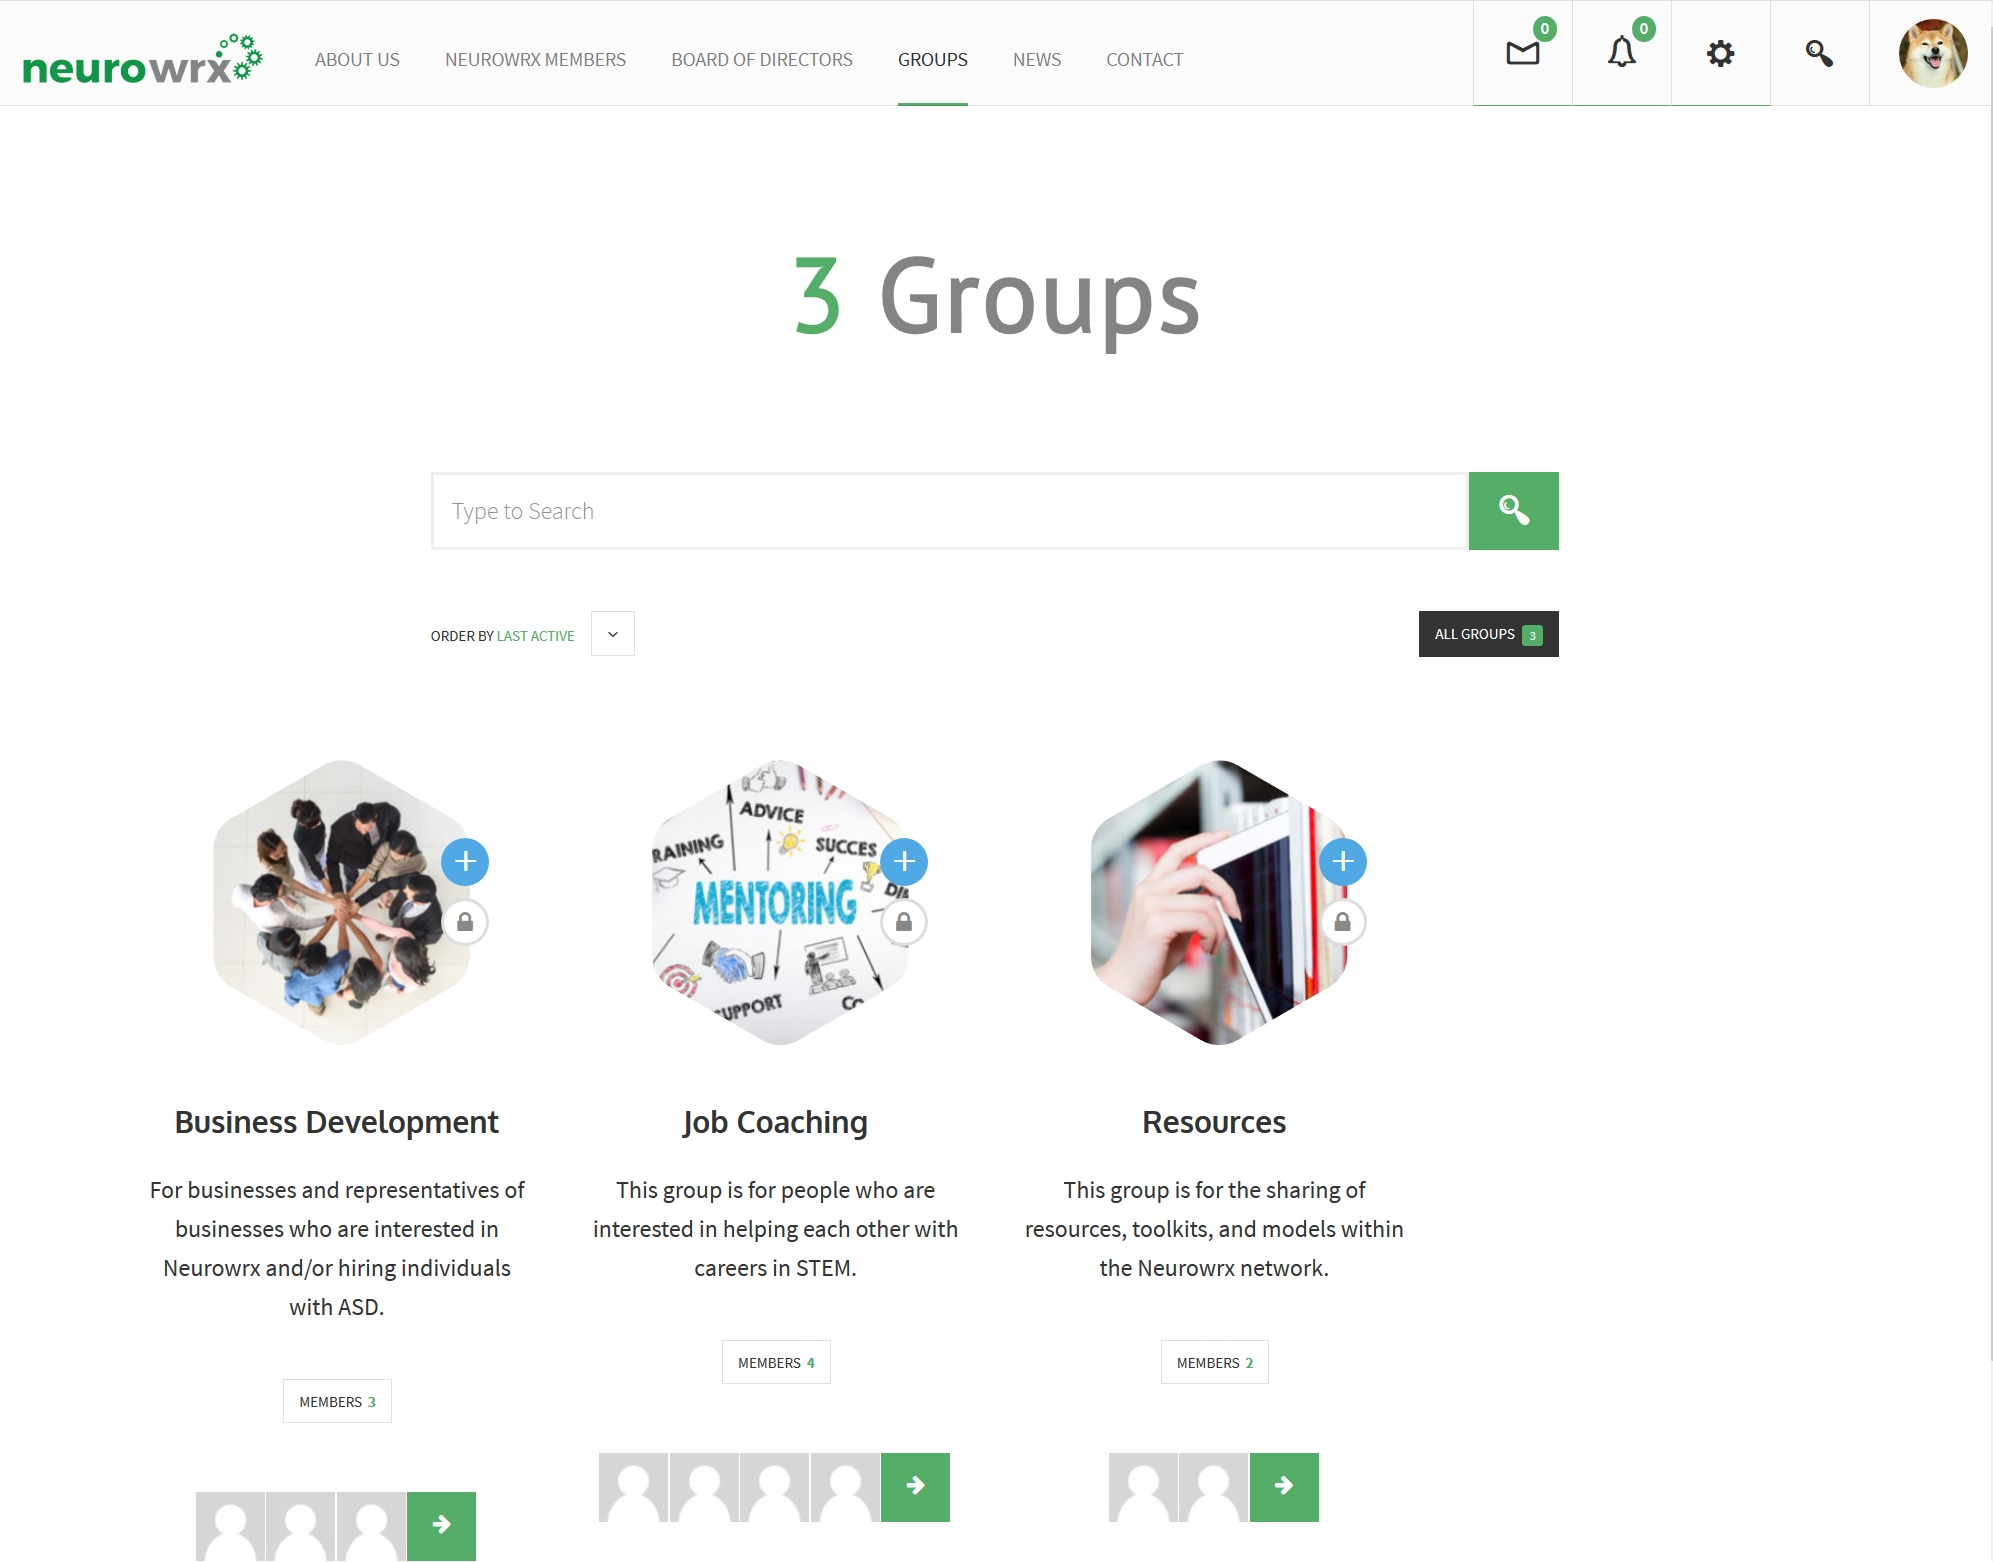
\includegraphics[scale=0.15]{images/allgroups.jpg}}}
    \qquad
    \subfloat{{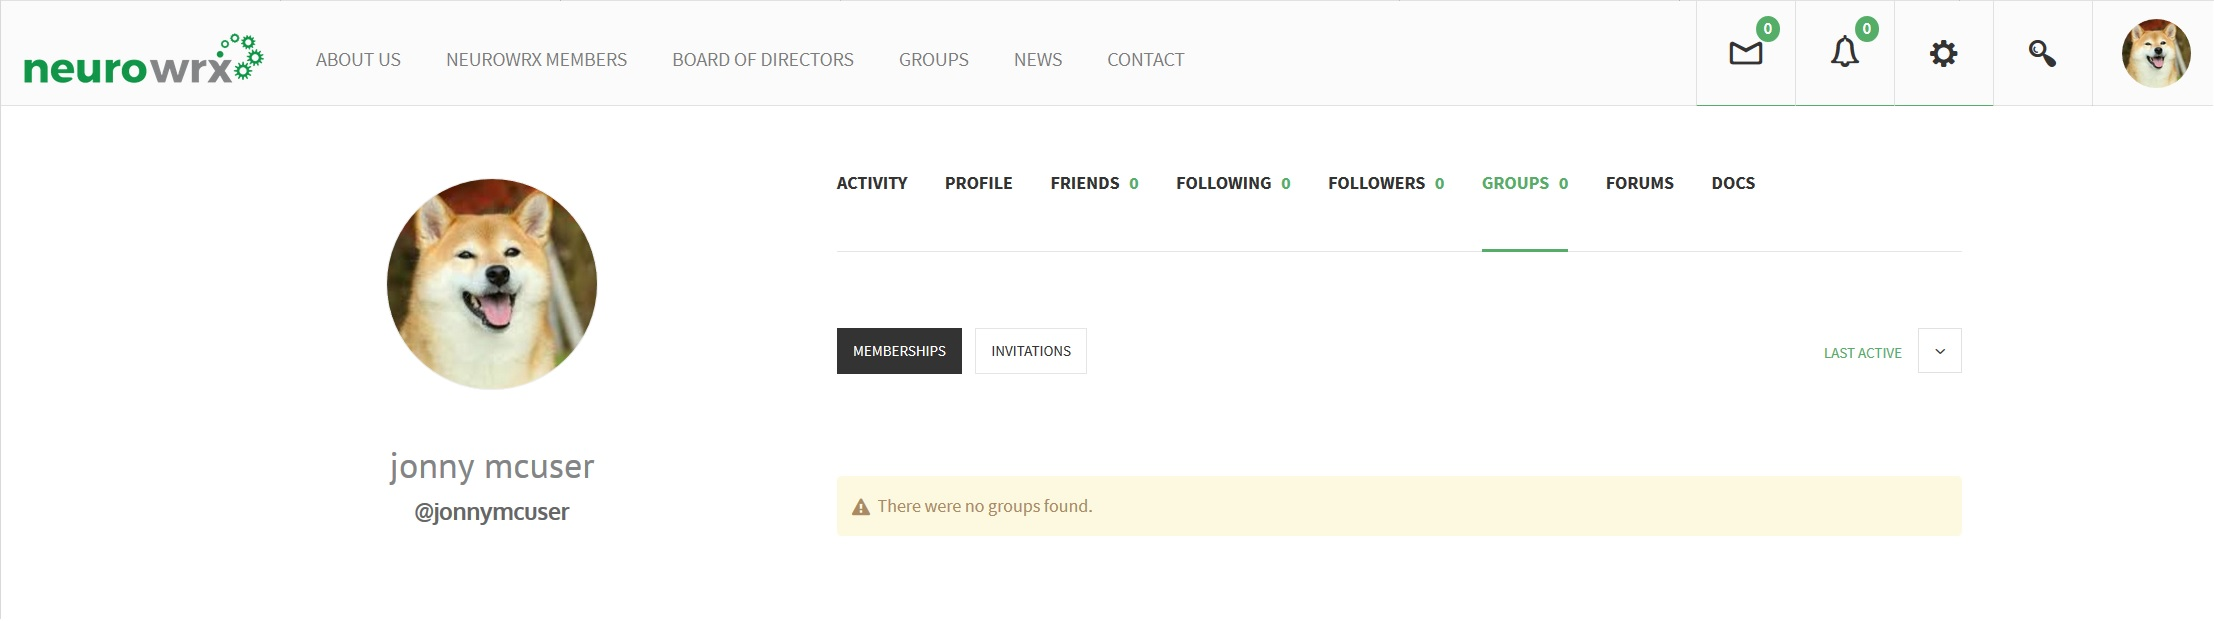
\includegraphics[scale=0.2]{images/usergroups.jpg}}}
    \caption{The general groups page accessed from the top panel (left) and the user's group page accessed though the dropdown menu (right)}
    \label{groupmenus}
\end{figure}

\subsubsection{Joining Groups}

\begin{flushleft}
To view the documents or discussions in a group, you must first be a member.  There are two ways to become a member of a group.  The first is that are invited by the group moderator, in which case the invite will be visible in the menu on the right in figure \ref{groupmenus}.  The second is that you apply for membership and your application is accepted by a group moderator.  This application is sent by clicking the plus sign in the blue circle to the upper right of the group avatar in the menu seen on the left in figure \ref{groupmenus}.  We will demonstrate both here. 
\end{flushleft}

\begin{flushleft}
When a request to join a particular group has been sent, by clicking on the send request button mentioned earlier, a red "x" appears in the upper right part of the plus symbol.  
\end{flushleft}

\begin{figure}[h]
    \centering
    
\includegraphics[scale=1]{images/requestsent.jpg}
    \caption{The request to join has been sent}
    \label{requestsent}
\end{figure}

\begin{flushleft}
Once an administrator accepts your request, you will receive a notification that your membership has been accepted in your notifications panel. See figure \ref{youaremember}.
\end{flushleft}

\begin{figure}[h]
    \centering
    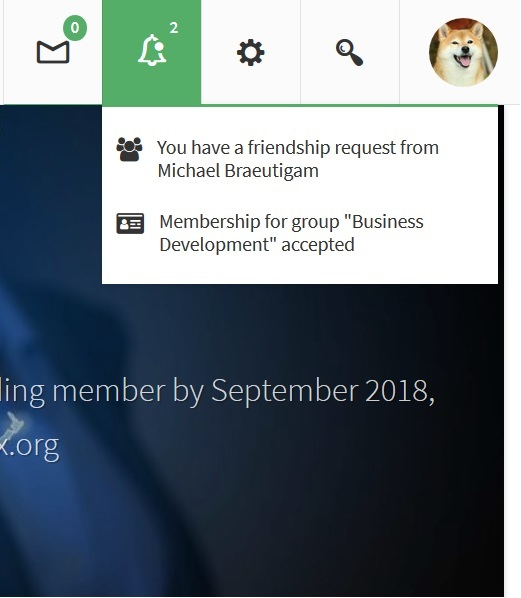
\includegraphics[scale=0.5]{images/youaremember.jpg}
    \caption{The member acceptance notification, at the bottom of the notification panel}
    \label{youaremember}
\end{figure}

\begin{flushleft}
The other way to end up a member of a group is for the administrator of a group to extend you an invitation, and for you to accept it.  When the invitation is sent, it will appear in your notification panel.  When you navigate to the page where an invitation can be accepted, you can either click the notification in the notification panel, or navigate to you personal groups page through the dropdown menu (see the right side of figure \ref{groupmenus}). 
\end{flushleft}

\begin{flushleft}
 In the second case, there is a button called "invitations" to the right of memberships that takes you to your pending invitations screen, which can either be accepted or rejected.  See figure \ref{invites}. 
\end{flushleft}

\begin{figure}[h]
    \centering
    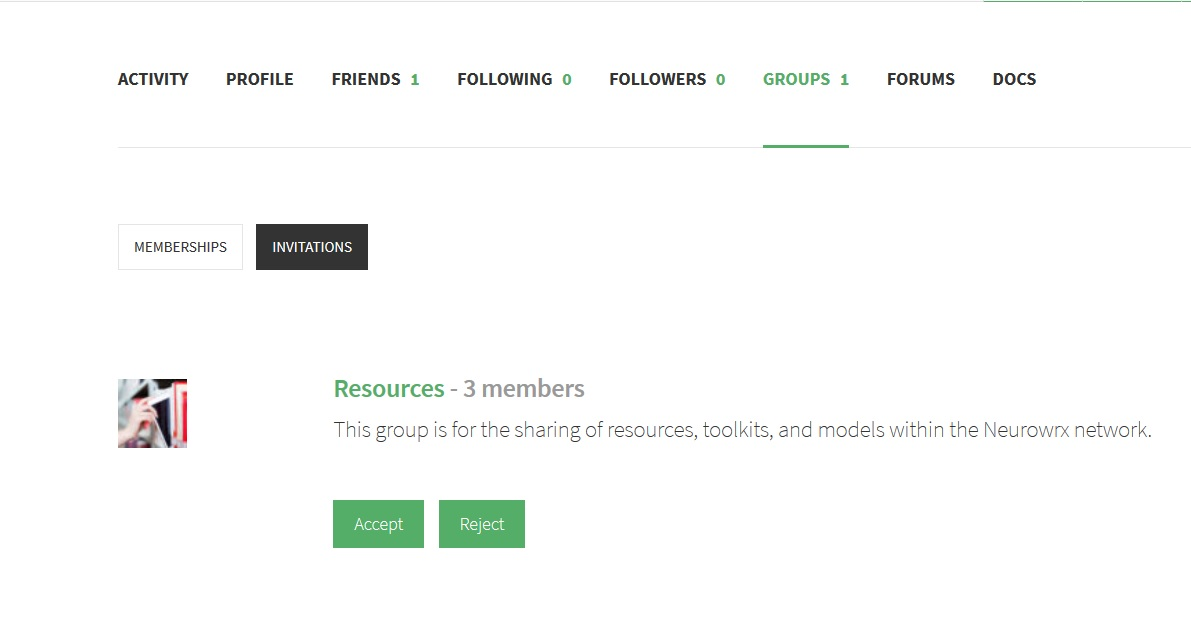
\includegraphics[scale=0.3]{images/invitations.jpg}
    \caption{Pending invitations screen}
    \label{invites}
\end{figure}

\subsubsection{Leaving Groups}

\begin{flushleft}
As with joining, there are multiple ways to leave a group.  The first is to go to the general groups page from the "Groups" link in the top panel (as in the left side of figure \ref{groupmenus}).  Once there, the groups that you are a member of (or have requested to be a member of) will have a red "x" at the top right of their blue "+" sign (see figure \ref{requestsent}).  If you click this icon, you membership to a group (or your request for membership) can be canceled, after confirmation. 
\end{flushleft}

\begin{flushleft}
The second way of leaving a group is to follow the same process as above, but from your personal groups page that is reached though the dropdown menu, as in the right side of figure \ref{groupmenus}.
\end{flushleft}

\begin{flushleft}
The third way is to go to the groups page itself, from either of the two previously mentioned menus, and click the green "leave group" button on the left hand side of the screen.  It is located below the groups avatar.  
\end{flushleft}

\begin{figure}[h]
    \centering
    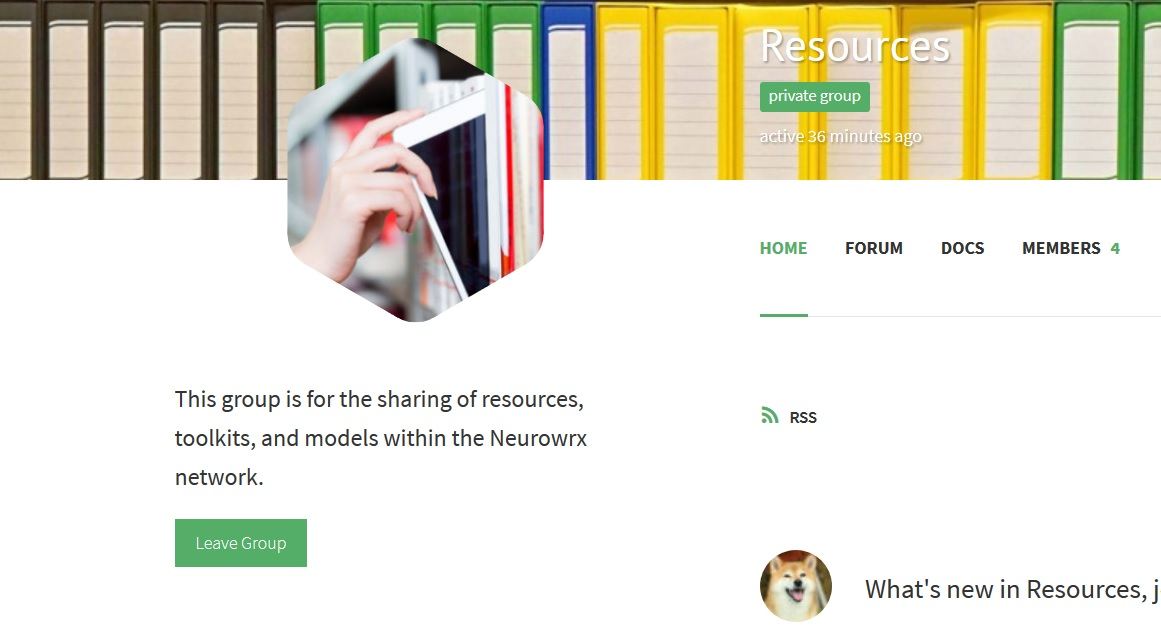
\includegraphics[scale=0.3]{images/leavegroup.jpg}
    \caption{The leave groups button on the groups main page}
    \label{leavegroup}
\end{figure}

\subsubsection{The groups activity feed}

\begin{flushleft}
Each group has an activity feed that is similar to the one associated with an individual user.  It aggregates automatically generated information associated with the group, and can also have items placed in it by the group members.  This can serve the purpose of enabling light informal banter, similar to twitter (see figure \ref{groupact}).  It is the default page that one sees when first clicking on a groups name (assuming that you are a member).  It can also be reached by clicking the home link from any of the other group pages. 
\end{flushleft}

\begin{figure}[H]
    \centering
    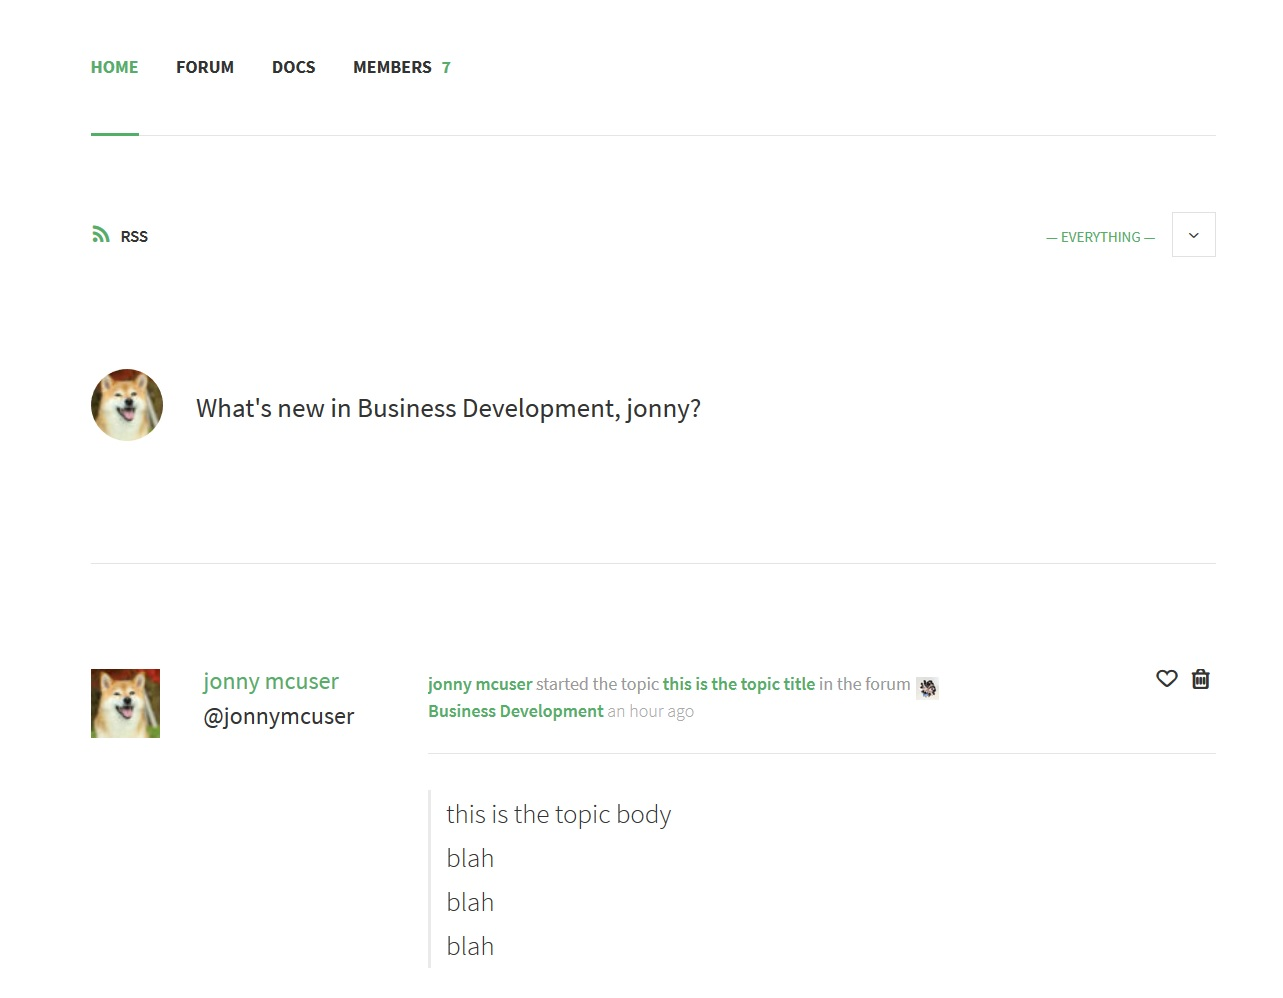
\includegraphics[scale=0.5]{images/groupactivity.jpg}
    \caption{A groups activity feed, note how the greeting is topic specific; just as the group is.}
    \label{groupact}
\end{figure}

\begin{flushleft}
The rest of the information about how a groups activity feed functions is contained in section \ref{Activity}.
\end{flushleft}

\subsubsection{The forum associated with a group} \label{groupforum}

\begin{flushleft}
A user is able to post in the forum associated with each group that they are a member of.  To view the forum, go to the main page of a group that you belong to.  There is a forum link right between the home and docs links.  (see figure \ref{forummain}).
\end{flushleft}




\begin{figure}[H]
    \centering
    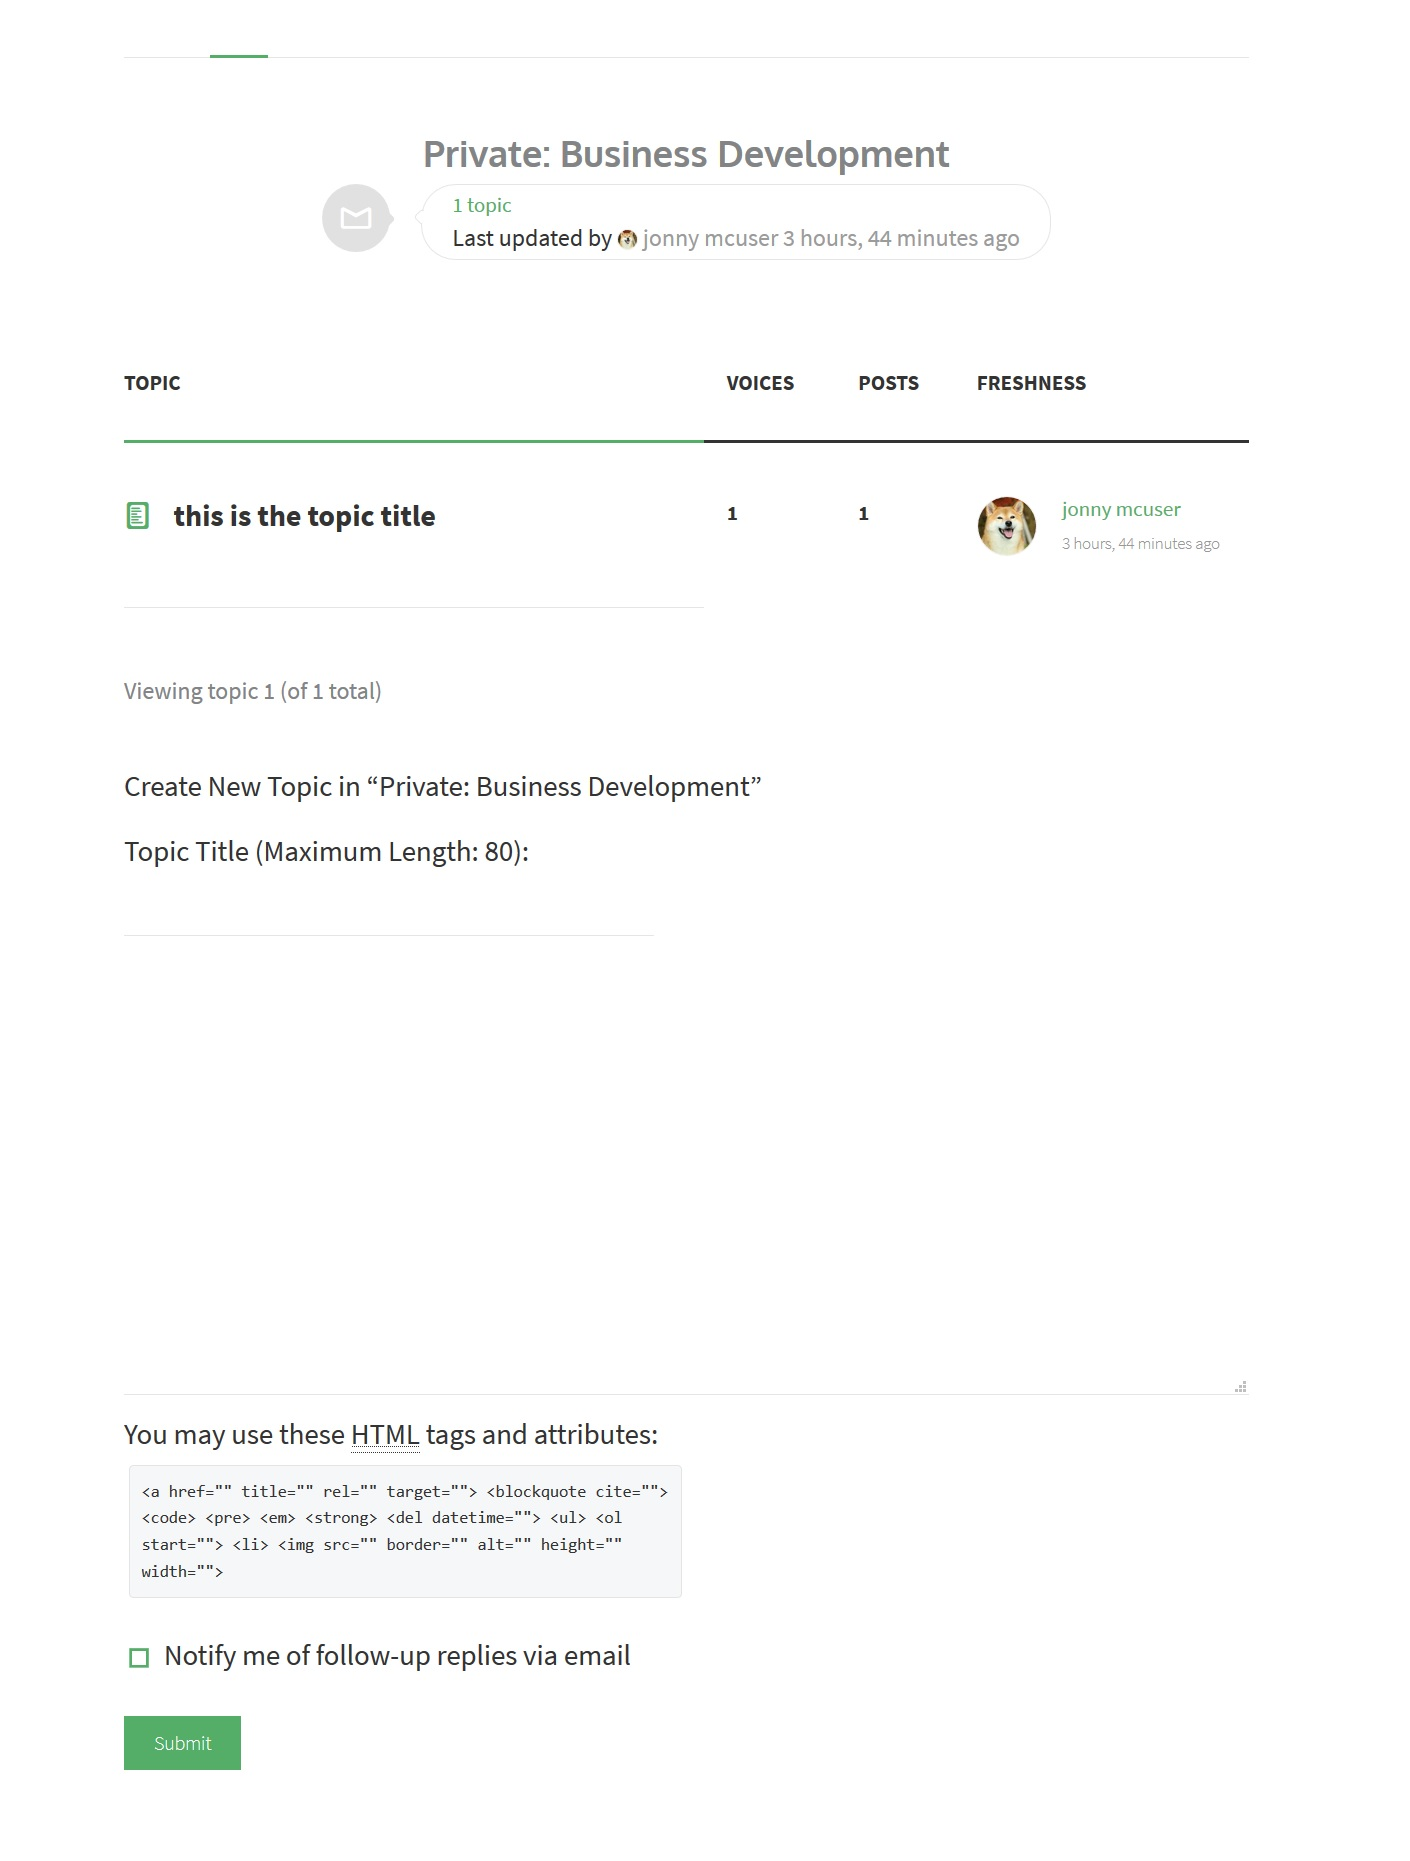
\includegraphics[scale=0.35]{images/forummain.jpg}
    \caption{The main page for the business development forum}
    \label{forummain}
\end{figure}

\begin{flushleft}
The group forums are only visible and available to members of the group.  The rest of the functionality of the forums is described in section \ref{Forums}.
\end{flushleft}


\subsubsection{The documents associated with a group}

\begin{flushleft}
Each group has a documents section associated with it.  The documents are pieces of rich (formatted) text that are created by group administrators and can (potentially, if the creator chooses) be commented on and edited by group members.  They are accessed by clicking on the docs link on the group home page (see figure \ref{groupsettings}).
\end{flushleft}

\begin{figure}[H]
    \centering
    
\includegraphics[scale=0.4]{images/groupsdocs.jpg}
    \caption{The document page for the job coaching group}
    \label{groupsdocs}
\end{figure}

\begin{flushleft}
If we click on the title of the document, we are brought to a page has tabs for reading, editing, and history viewing (see figure \ref{docpage}).  We also have the ability to comment on the document, as well as comment on other peoples comments, providing the document creator allows it. 
\end{flushleft}

\begin{figure}[H]
    \centering
    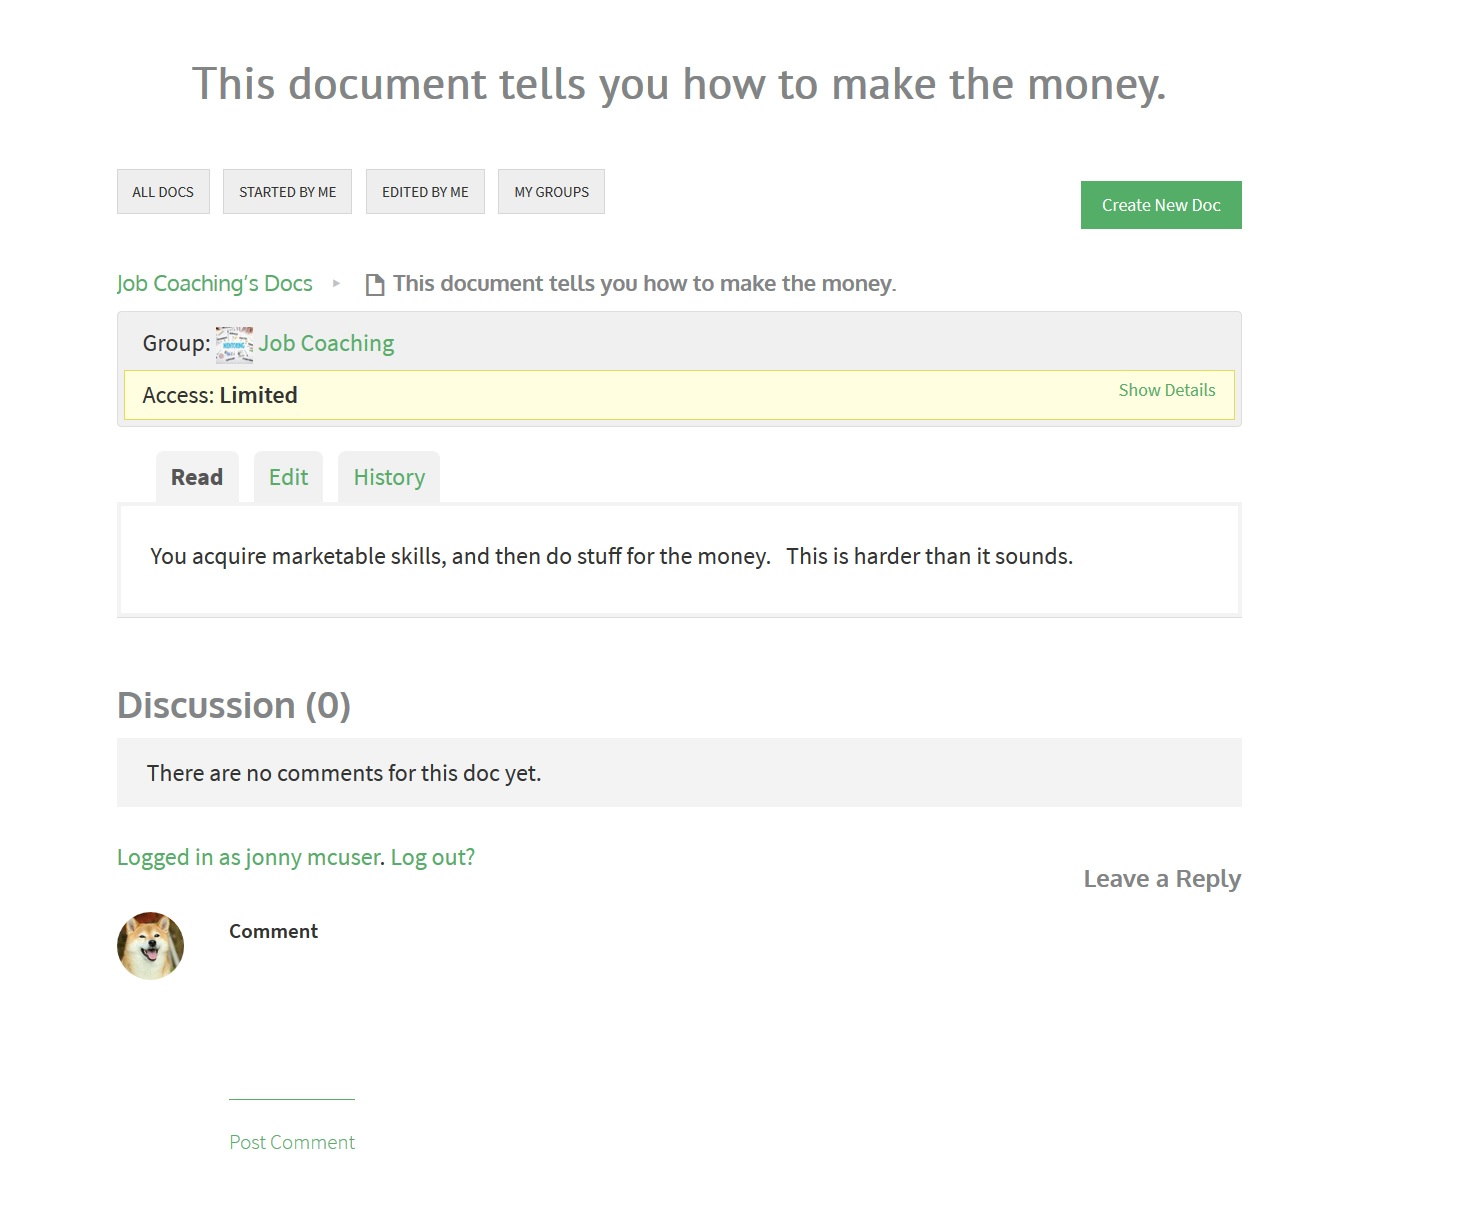
\includegraphics[scale=0.5]{images/docpage.jpg}
    \caption{The page of a the document "This document tells you how to make the money"}
    \label{docpage}
\end{figure}

\begin{flushleft}
If we add a couple lines to this document in the editing tab, we can see the changes in the documents history tab.  After the changes have been made, clicking the green "save" button at the bottom commits them.  Then clicking the "history" tab allows us to view the documents editing history (see figure \ref{edithistory}).
\end{flushleft}

\begin{figure}[H]
    \centering
    \subfloat{{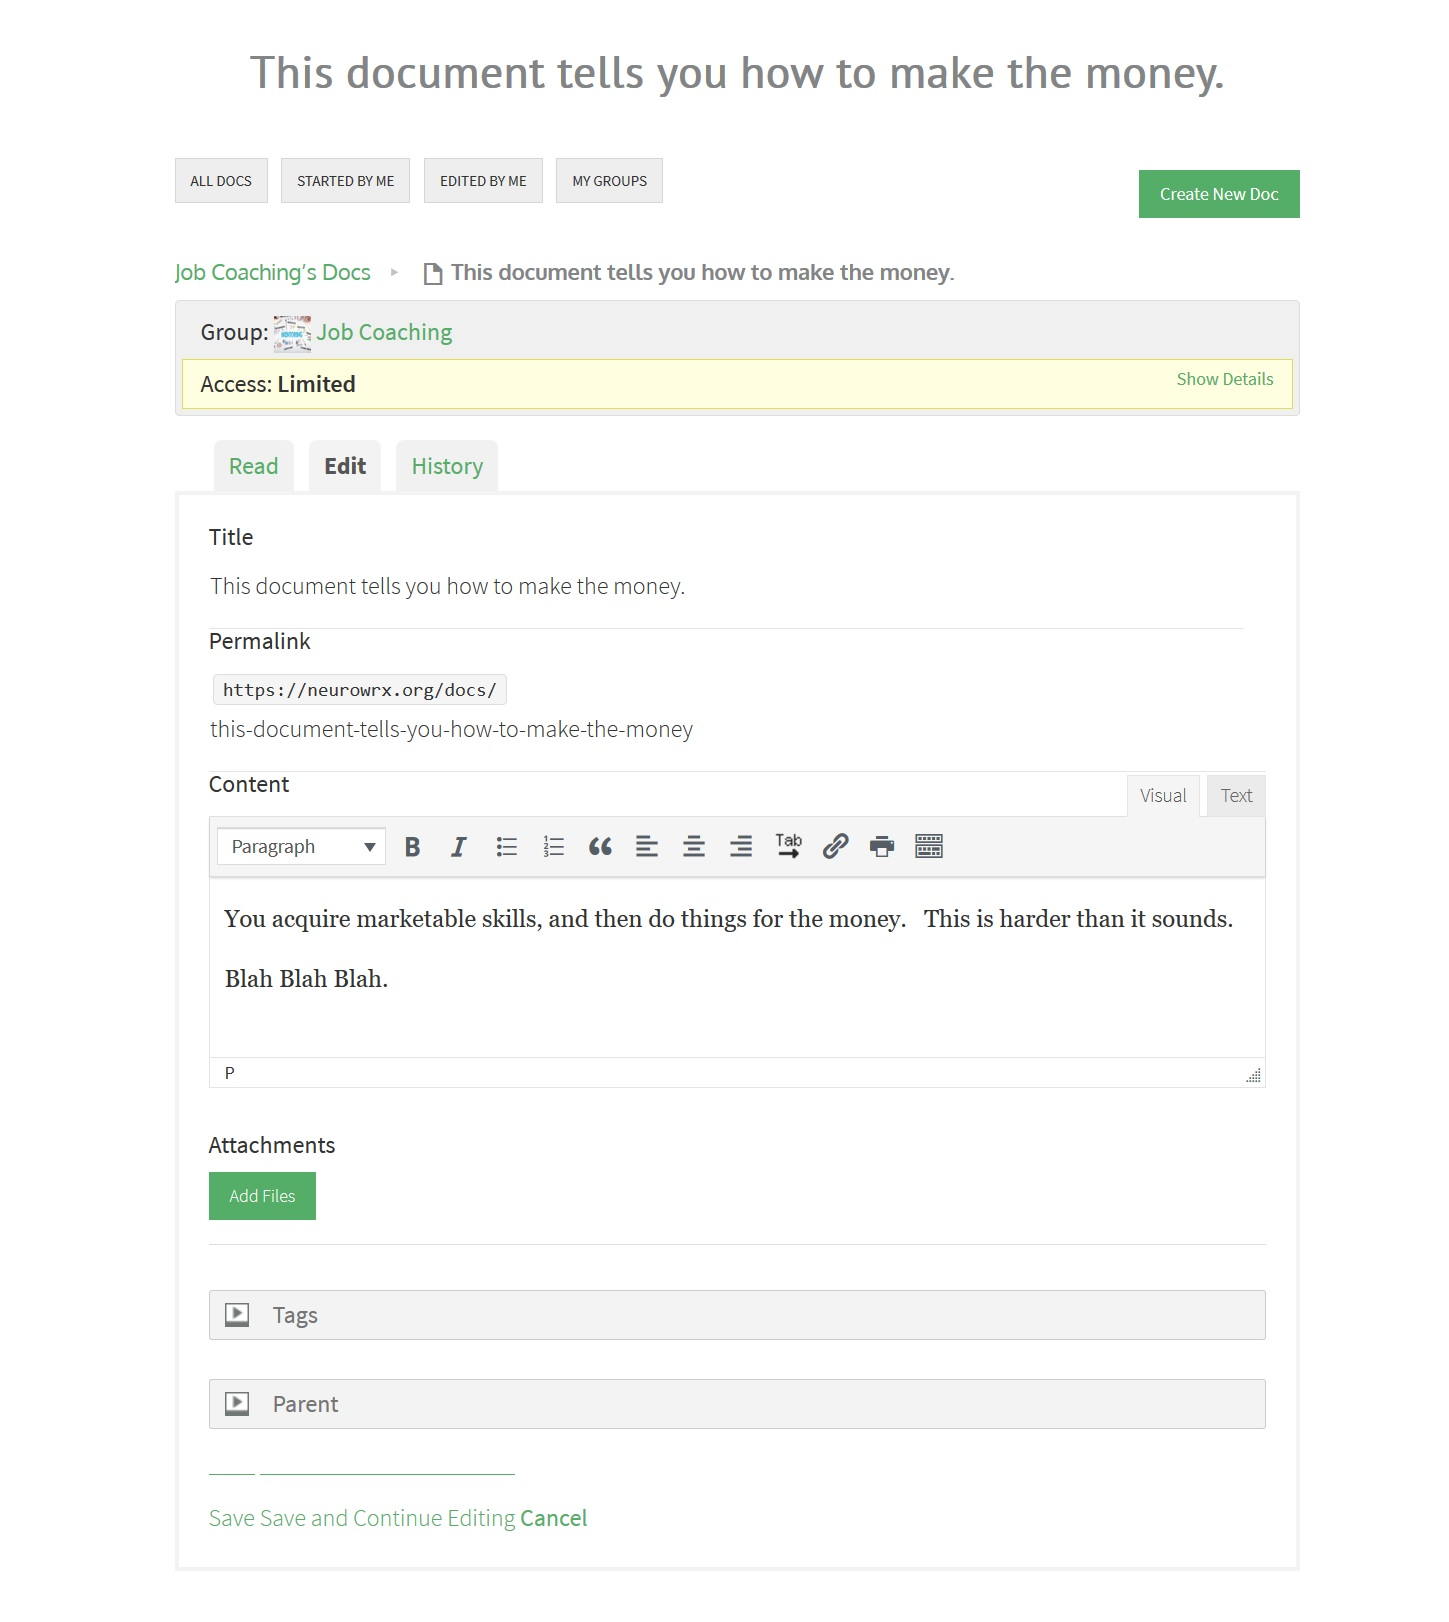
\includegraphics[scale=0.30]{images/docedit.jpg}}}
    \qquad
    \subfloat{{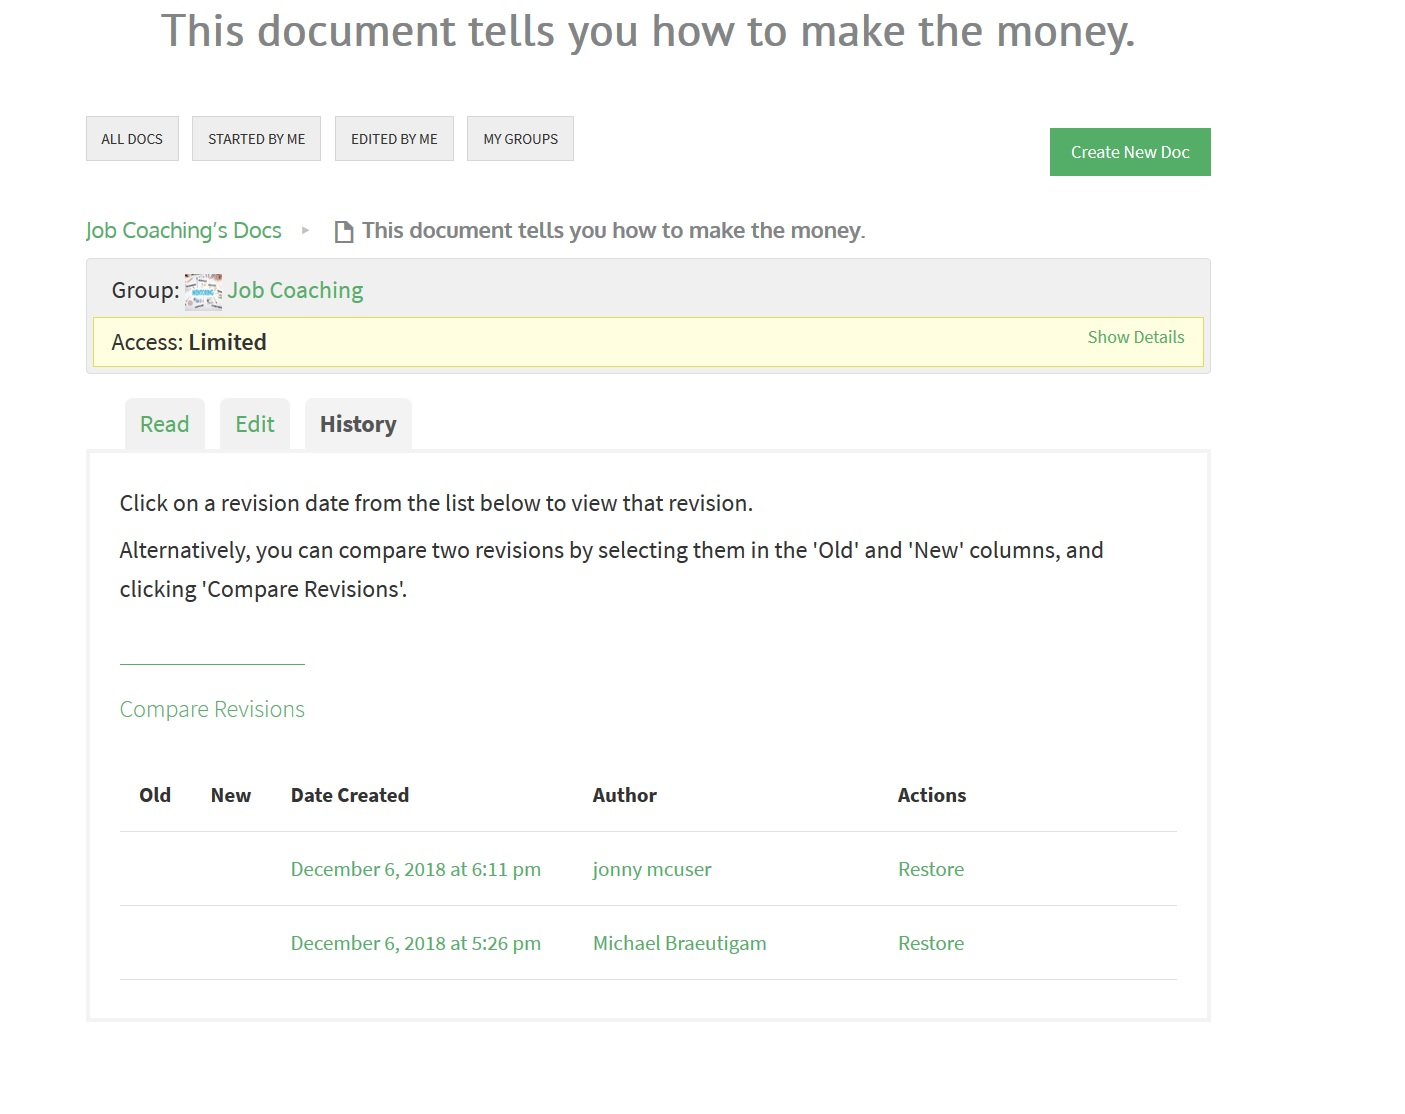
\includegraphics[scale=0.30]{images/dochist.jpg}}}
    \caption{The editing and history windows.}
    \label{edithistory}
\end{figure}

\begin{flushleft}
As one can see on the history page, each edit event, as well as the user that performed it, is listed.  You can restore the document to any previous version by clicking the restore link and confirming your choice. 
\end{flushleft}

\subsubsection{Viewing the members of a group}

\begin{flushleft}
The members page of a group contains a profile picture of every member (which can only be viewed if you are a member, of course) contain a profile picture of every member, along with small buttons that enable you to add (or remove) people as friends or follow them. 
\end{flushleft}


\begin{figure}[H]
    \centering
    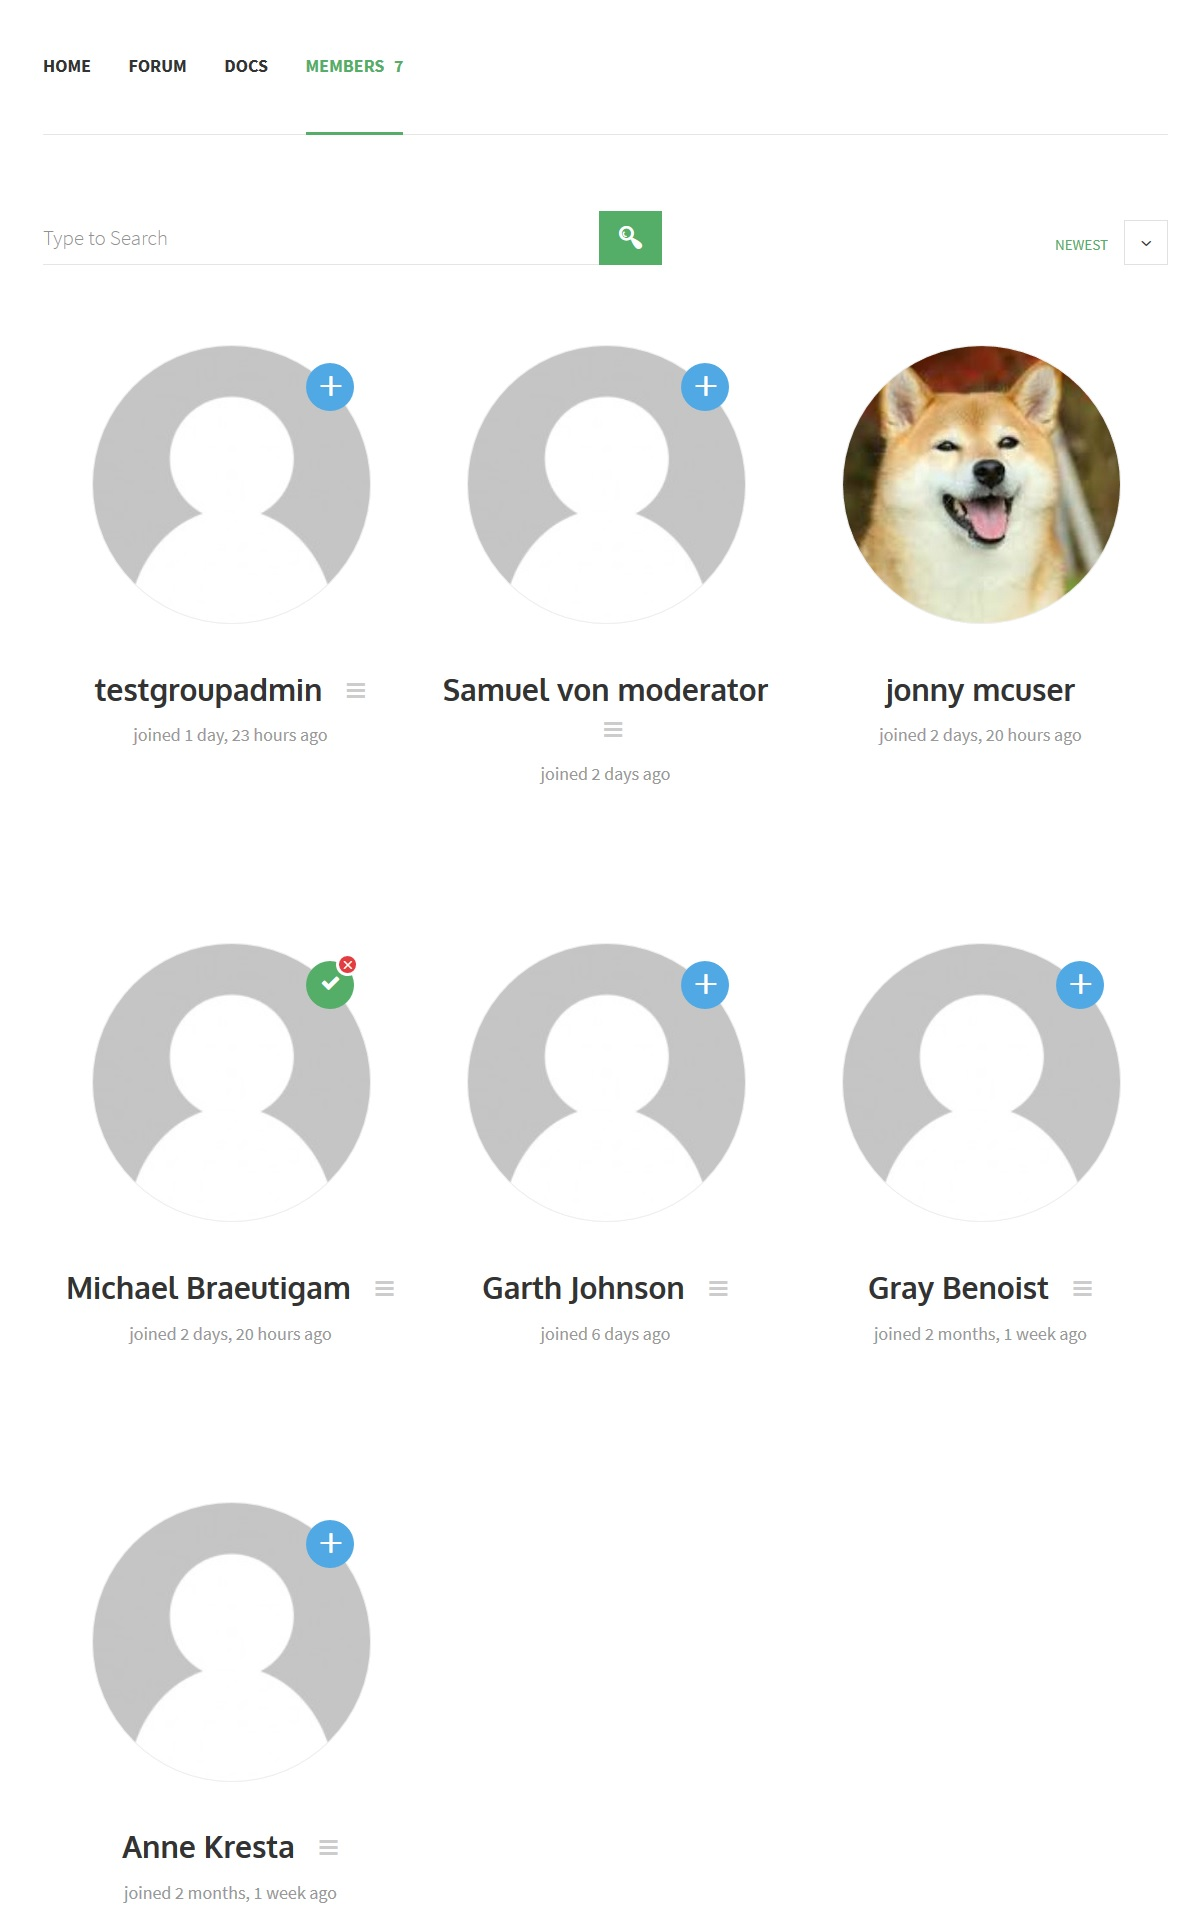
\includegraphics[scale=0.25]{images/groupmembers.jpg}
    \caption{The members page.  Notice how the profile pictures are an instance of what was described in figure \ref{profilepics}}
    \label{fig:my_label}
\end{figure}

\begin{flushleft}
All of these profile pictures are also links to their user's page.  The function on that page described elsewhere can be accessed through them.
\end{flushleft}

\subsection{Forums} \label{Forums}
The forums on the site provide an environment to have a more structured, involved and uncluttered conversation that the activity feeds.  They are intended to be organized around specific topics.  There are forums associated with particular groups, which can be accessed by the process described in section \ref{groupforum}.  There is also a general forums page that lists all forums that is accessible though the top bar of the site (while logged in).  


\subsubsection{The main forum page and creating topics} \label{doggopost}
\begin{flushleft}
As you can see in figure \ref{forumpage}, there is already a post in the forum, with title "this is the topic title".  If we click on the title, it will take us to the post's content.  If we wanted to create a new topic, we could use the form at the bottom of the page to enter it's title and initial post, and then click the green submit button.  As the page tells us, we can use html attribute tags to enrich the content slightly.
\end{flushleft}



\begin{figure}[H]
    \centering
    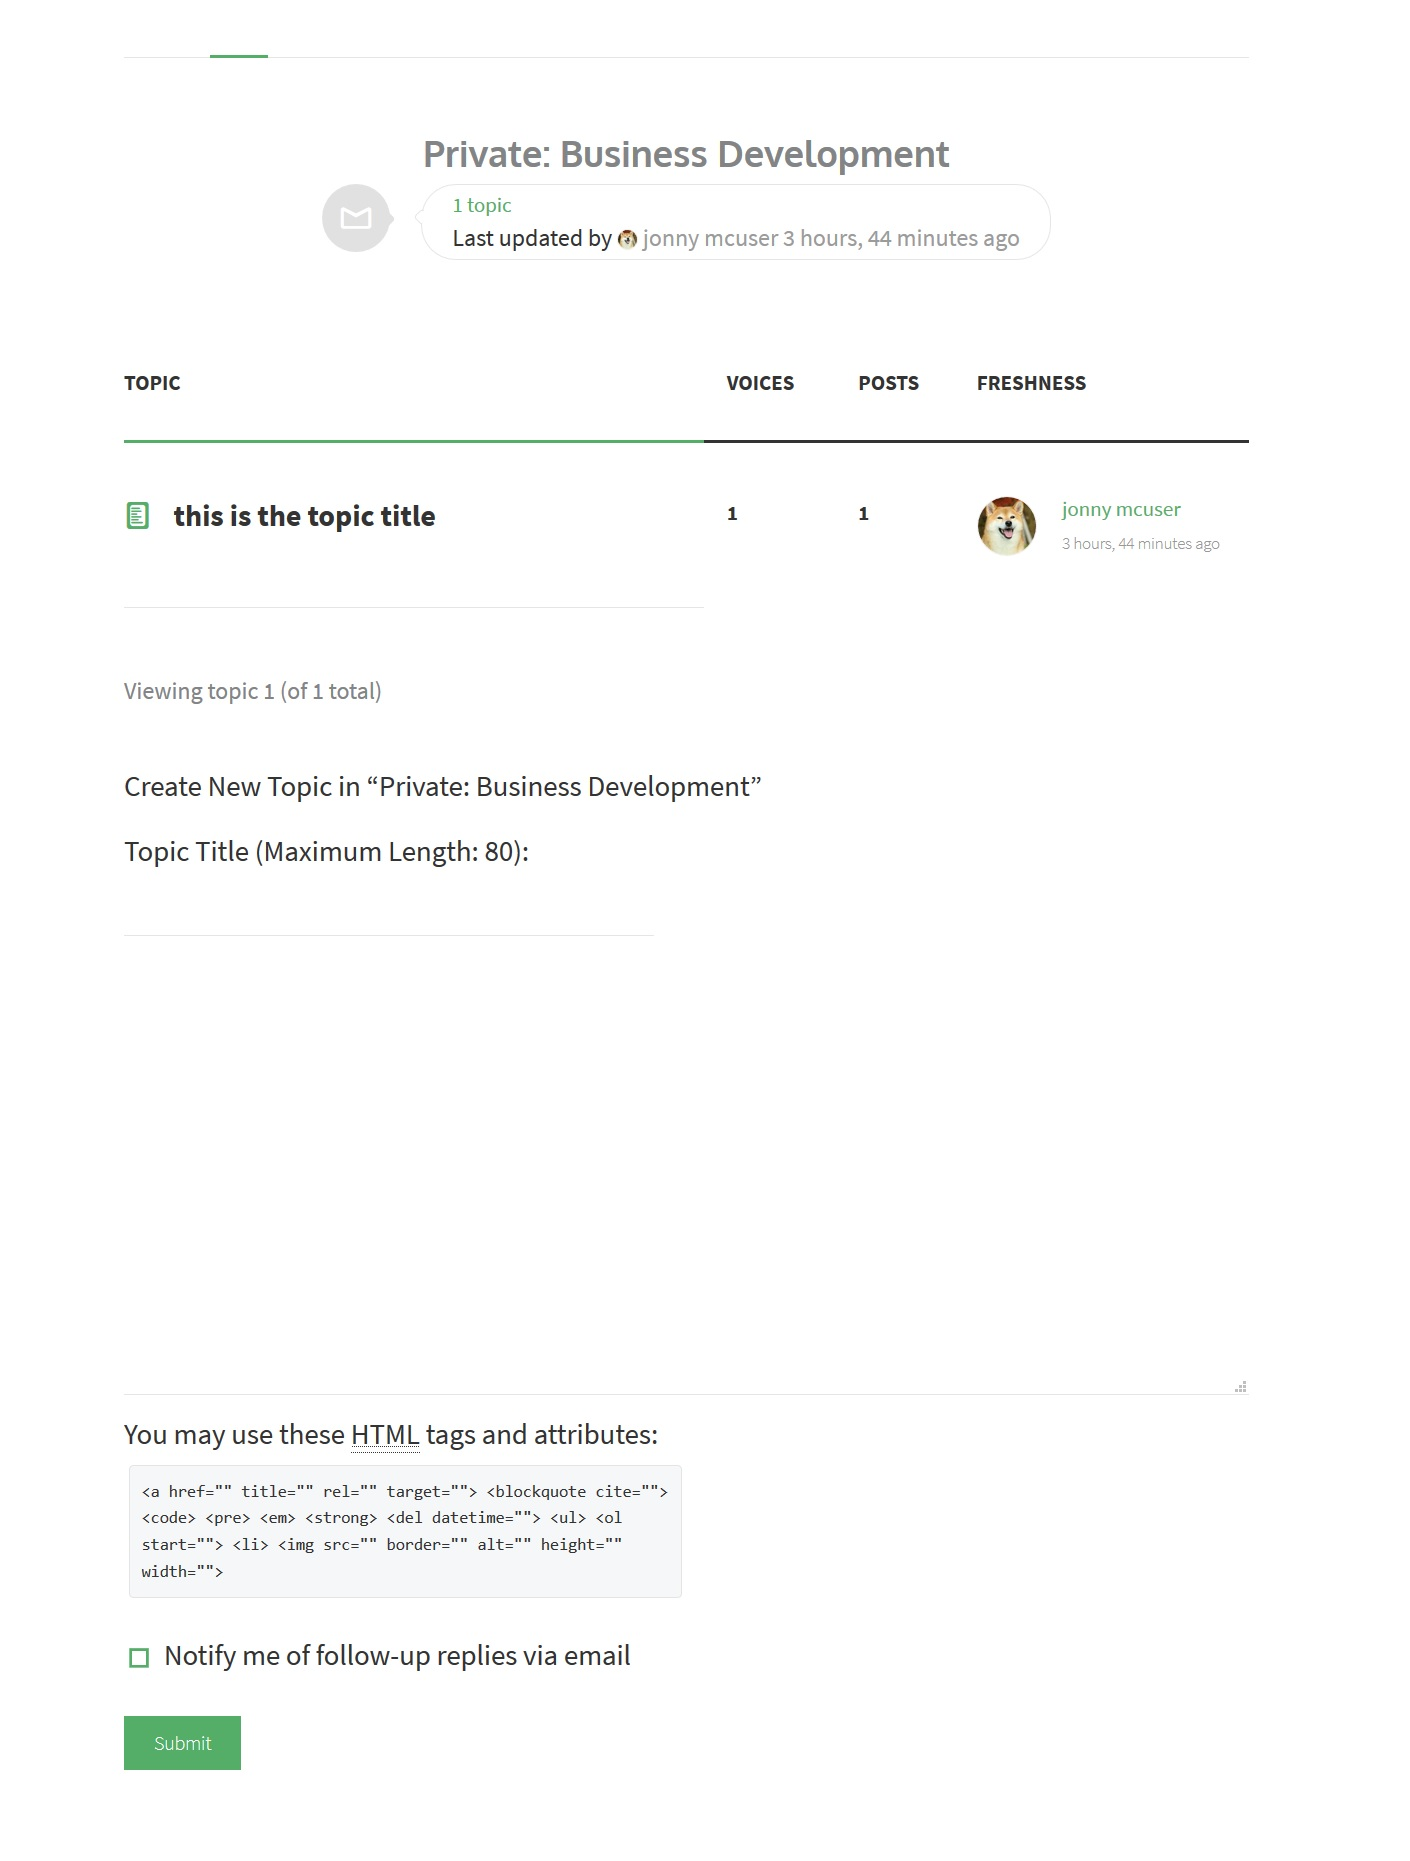
\includegraphics[scale=0.3]{images/forummain.jpg}
    \caption{The main page for the business development forum}
    \label{forumpage}
\end{figure}


\begin{flushleft}
For example, if we created a topic "How do I make the money?", with initial post "Is it ok that I am a dog?", and include our profile picture.  We would write the following (note the use of the html tag.  If you don't know html, pehaps look up tutorials on the specific tags listed in the box in figure \ref{forumpage}): 
\end{flushleft}

\begin{figure}[H]
    \centering
    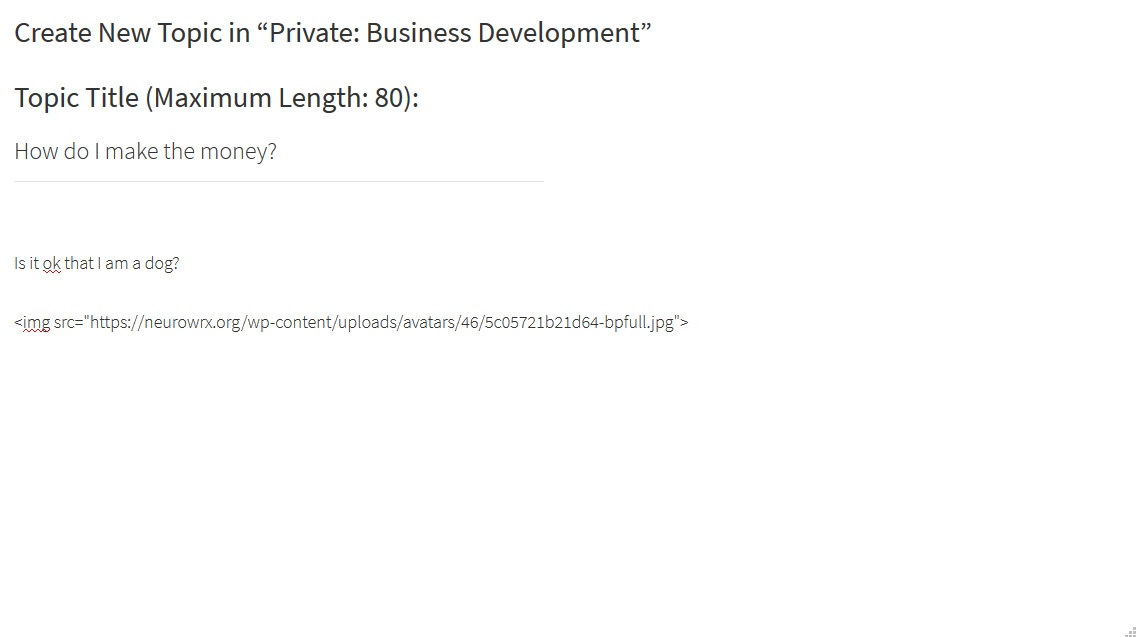
\includegraphics[scale=0.4]{images/newtopic.jpg}
    \caption{The new topic as we enter it}
    \label{newtopic1}
\end{figure}

\begin{flushleft}
Which would result in this if posted:
\end{flushleft}

\begin{figure}[H]
    \centering
    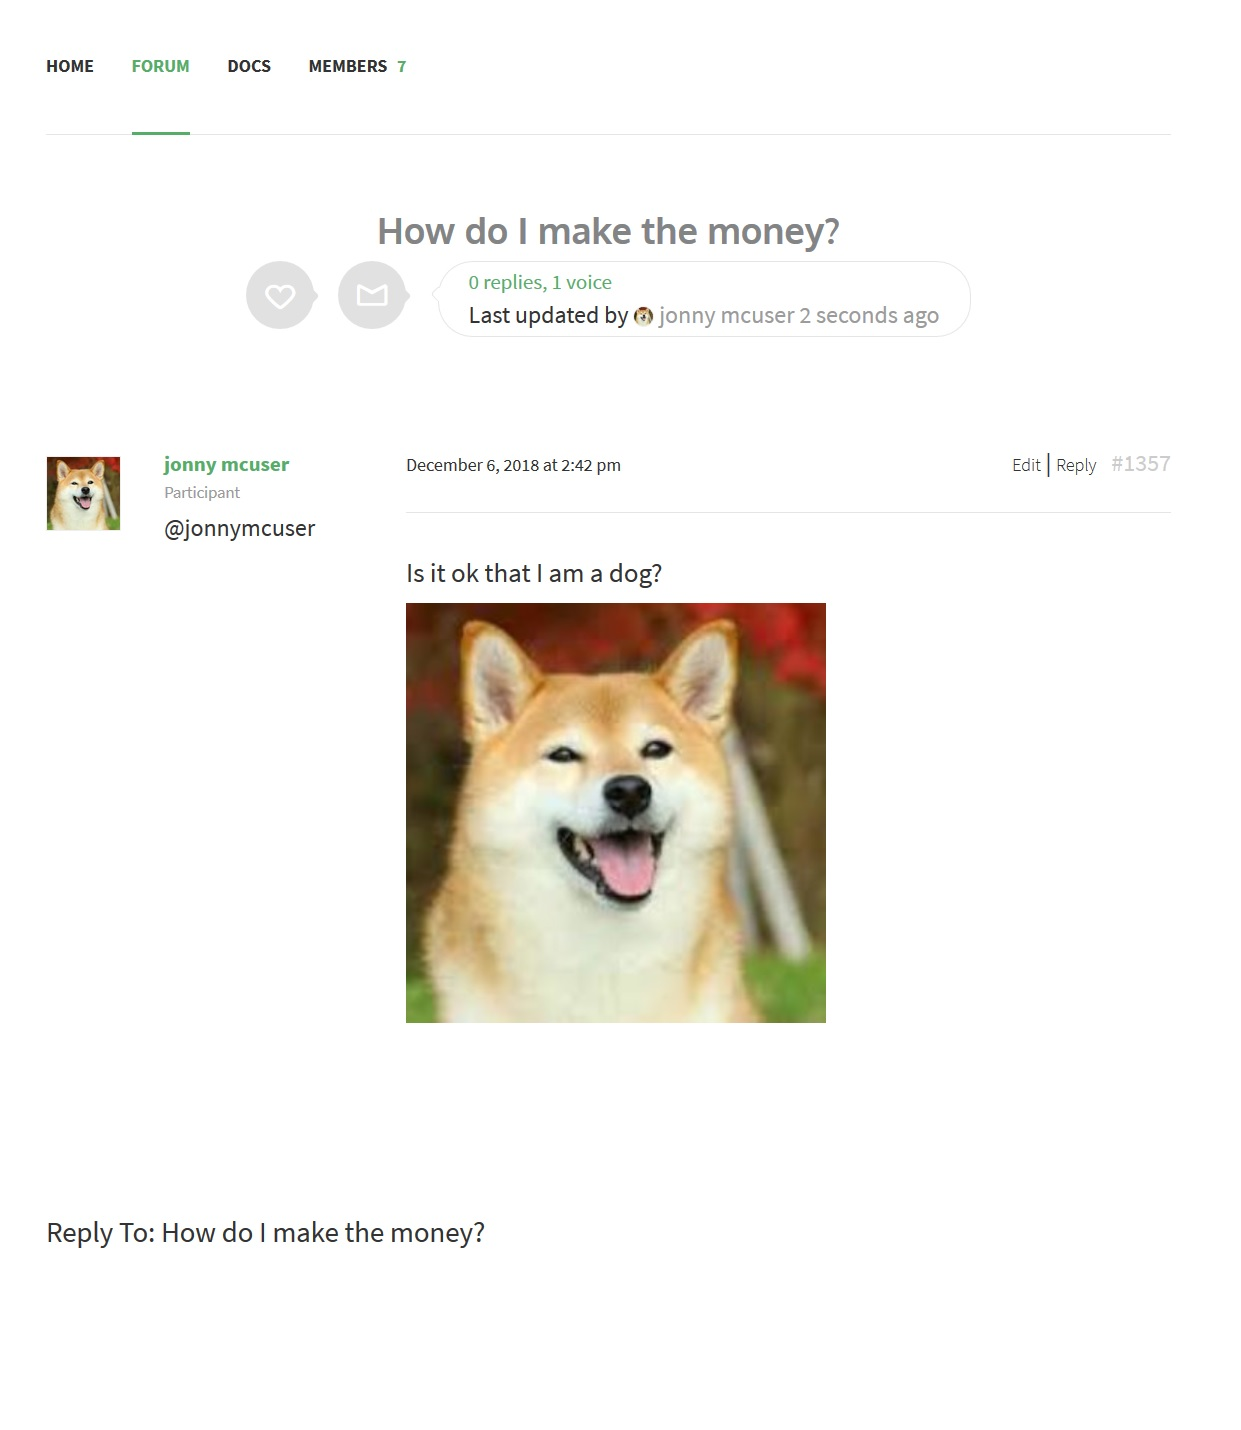
\includegraphics[scale=0.4]{images/viewnewpost.jpg}
    \caption{The new topic as other people will see it, ready to be replied to}
    \label{newtopic2}
\end{figure}

\subsubsection{Viewing and replying to existing topics}

\begin{flushleft}
If we saw the topic in the previous section on the main forum page (How do I make the money?) and wished to reply to it as another user (or even ourselves, as we can reply to our own posts), we would simply add the text (or whatever else, like pictures) into the reply section at the bottom of the viewing page, and click submit. 
\end{flushleft}

\begin{figure}[H]
    \centering
    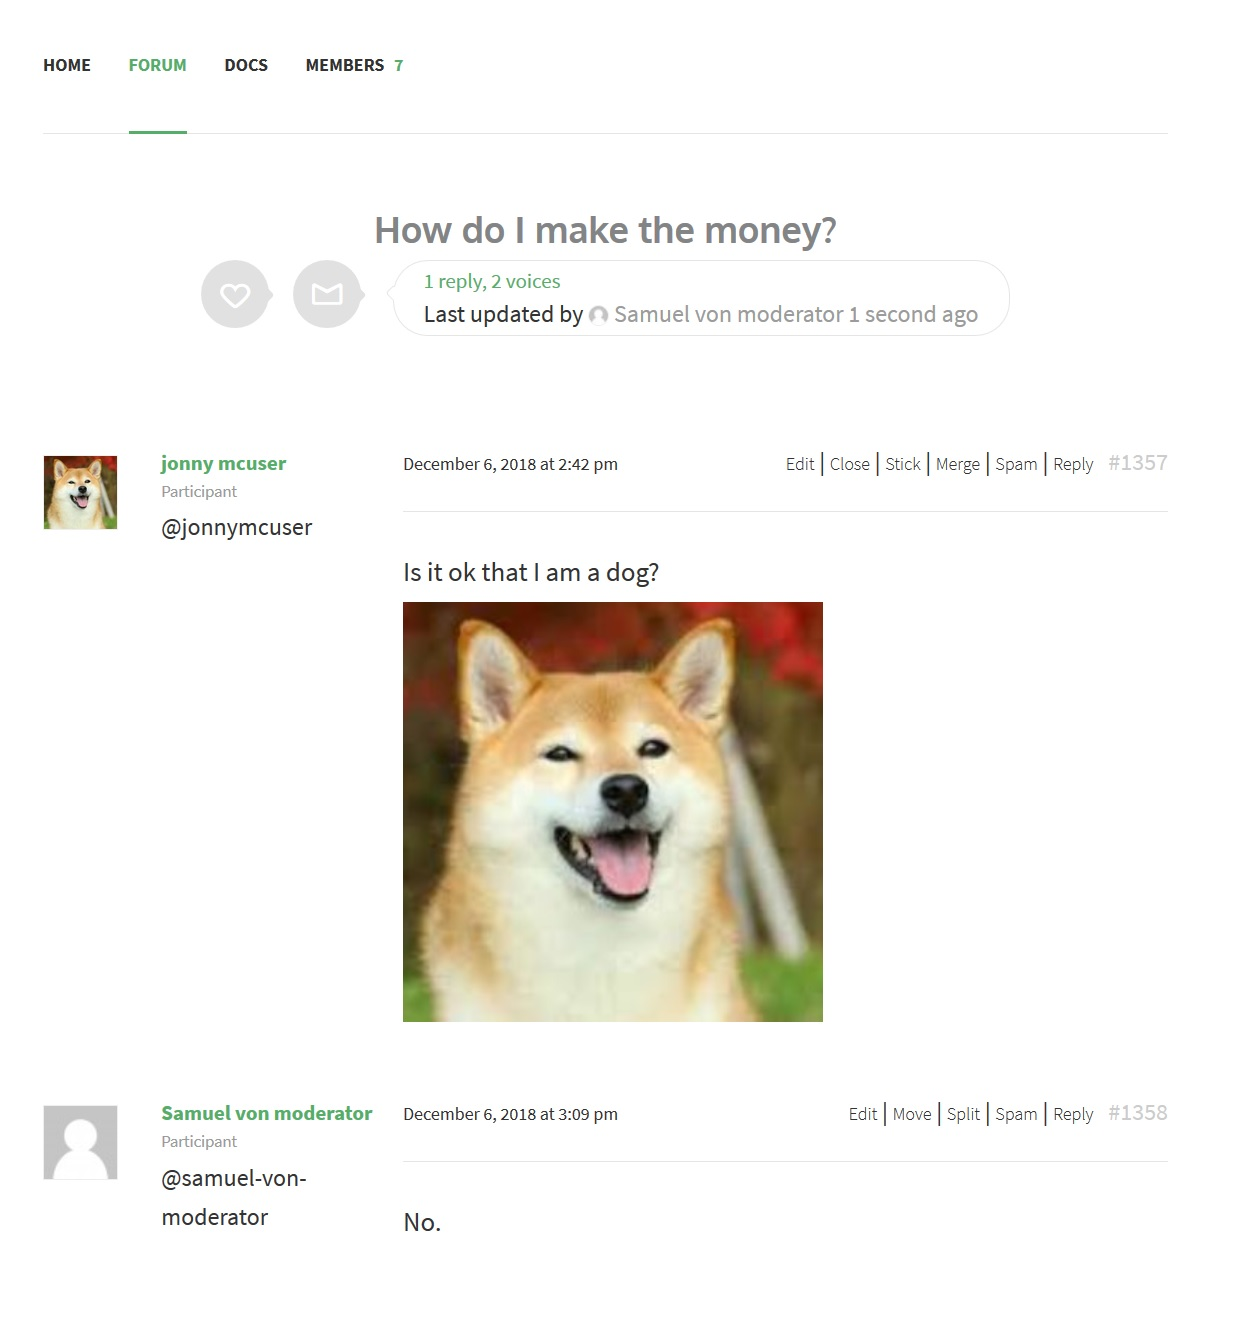
\includegraphics[scale=0.4]{images/nodoggo.jpg}
    \caption{A user (a moderator in this case) replying to a topic}
    \label{nodoggo}
\end{figure}




\subsection{Account Settings}
\begin{flushleft}
Each account has some user controllable account settings that can be accessed though the last link on the profile pic dropdown menu.  The different sections are as follows:
\end{flushleft}


\begin{itemize}
    \item General:  Allows the change of the email address connected with the accound, as well as the password
    \item Email: Contains a long list of toggles that control what kind of events generate notification emails
    \item Profile Visibility: Controls whether or not other users can see your name and/or gender
\end{itemize}

\begin{flushleft}
The first page (the general section) is the only one that wants for explanation.  On it, you are presented with a form with fields for your current password, email, a new password and a new password confirmation (see figure \ref{settings}).

\end{flushleft}

\begin{figure}[H]
    \centering
    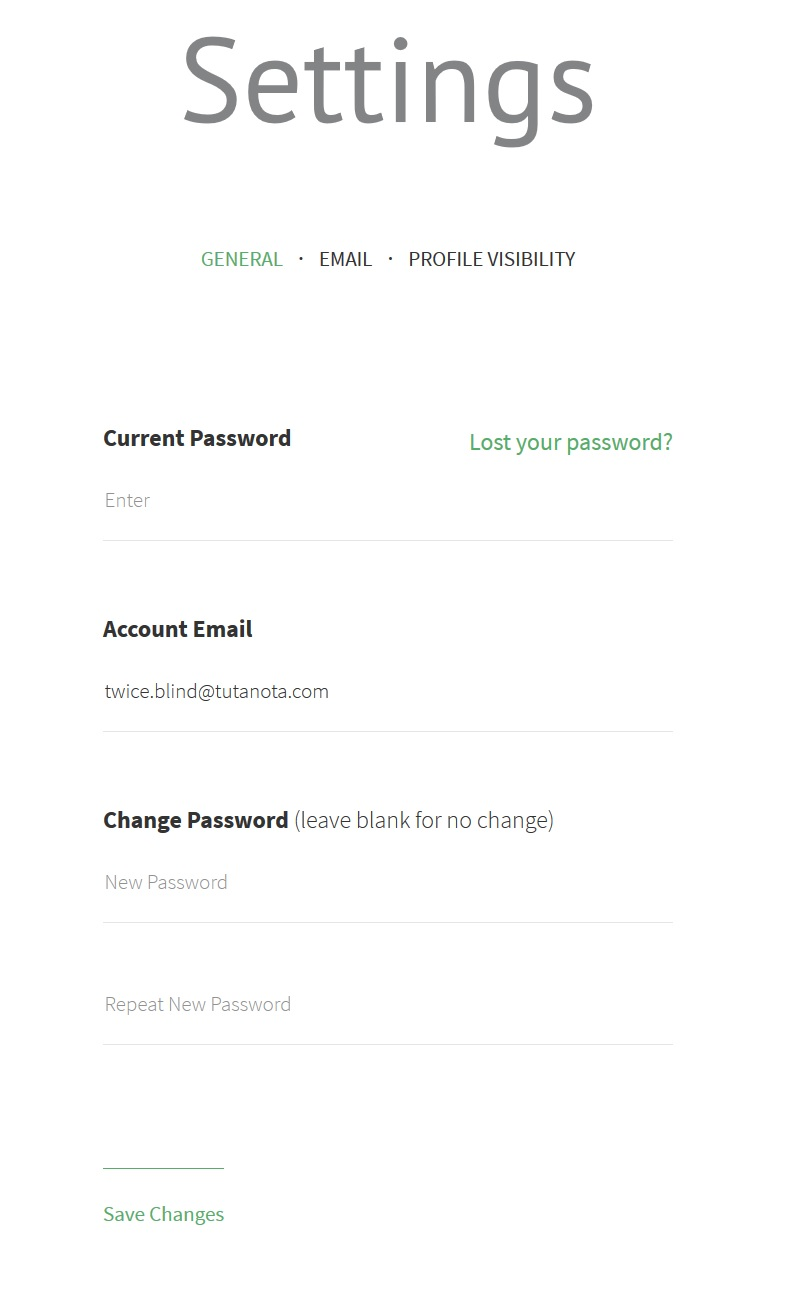
\includegraphics[scale=0.3]{images/settings.jpg}
    \caption{The general settings form}
    \label{settings}
\end{figure}

\begin{flushleft}
To make any changes to this form, the correct account password must be entered into the top field.  Then whatever changed the user wishes to be made can be made to the other fields.  Once the form with the correct password and desired changes has been filled out, clicking the "save changes" button will do so. 
\end{flushleft}



\section{Group Moderators} \label{Moderators}

\begin{flushleft}
Group moderators have elevated access and responsibilities.  They have the ability to remove or alter content posted by users.  The rules governing this are a matter of policy and not defined in this document.  The following only covers how these things are to be achieved in the application itself. 
\end{flushleft}

\begin{flushleft}
The additional functionality associated with moderation is accessed though additional links in the forum section.  If we are viewing a particular post, such as the one made in section \ref{doggopost}, these new links appear to the left of the reply button that ordinary users have access to (see figure \ref{modpowers}).  
\end{flushleft}

\begin{figure}[H]
    \centering
    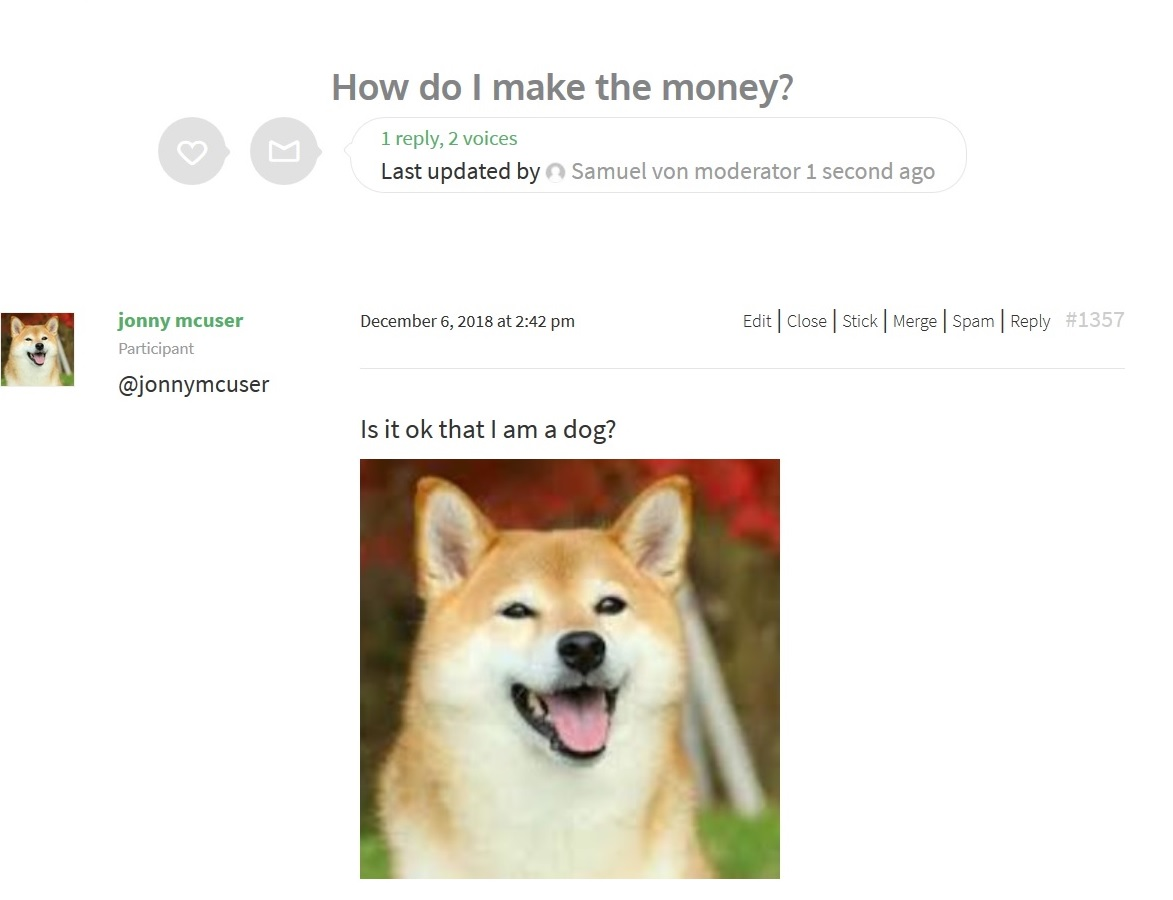
\includegraphics[scale=0.5]{images/moderatorpostview.jpg}
    \caption{The powers associated with moderation}
    \label{modpowers}
\end{figure}

\begin{flushleft}
We will go through these additional features in the following subsections. 
\end{flushleft}

\subsection{Editing Posts}

\begin{flushleft}
Upon clicking the edit button, a window appears that could be seen as an enhanced version of the posting window.  It not only allows you to change the content of the post itself to whatever you wish, but also to move it to other forums with the forums dropdown menu, make the topic sticky (so that it stays at the top of the list of topics), or change the status of the topic to closed, spam, trash or pending (this will be discussed later). 
\end{flushleft}

\begin{figure}[H]
    \centering
    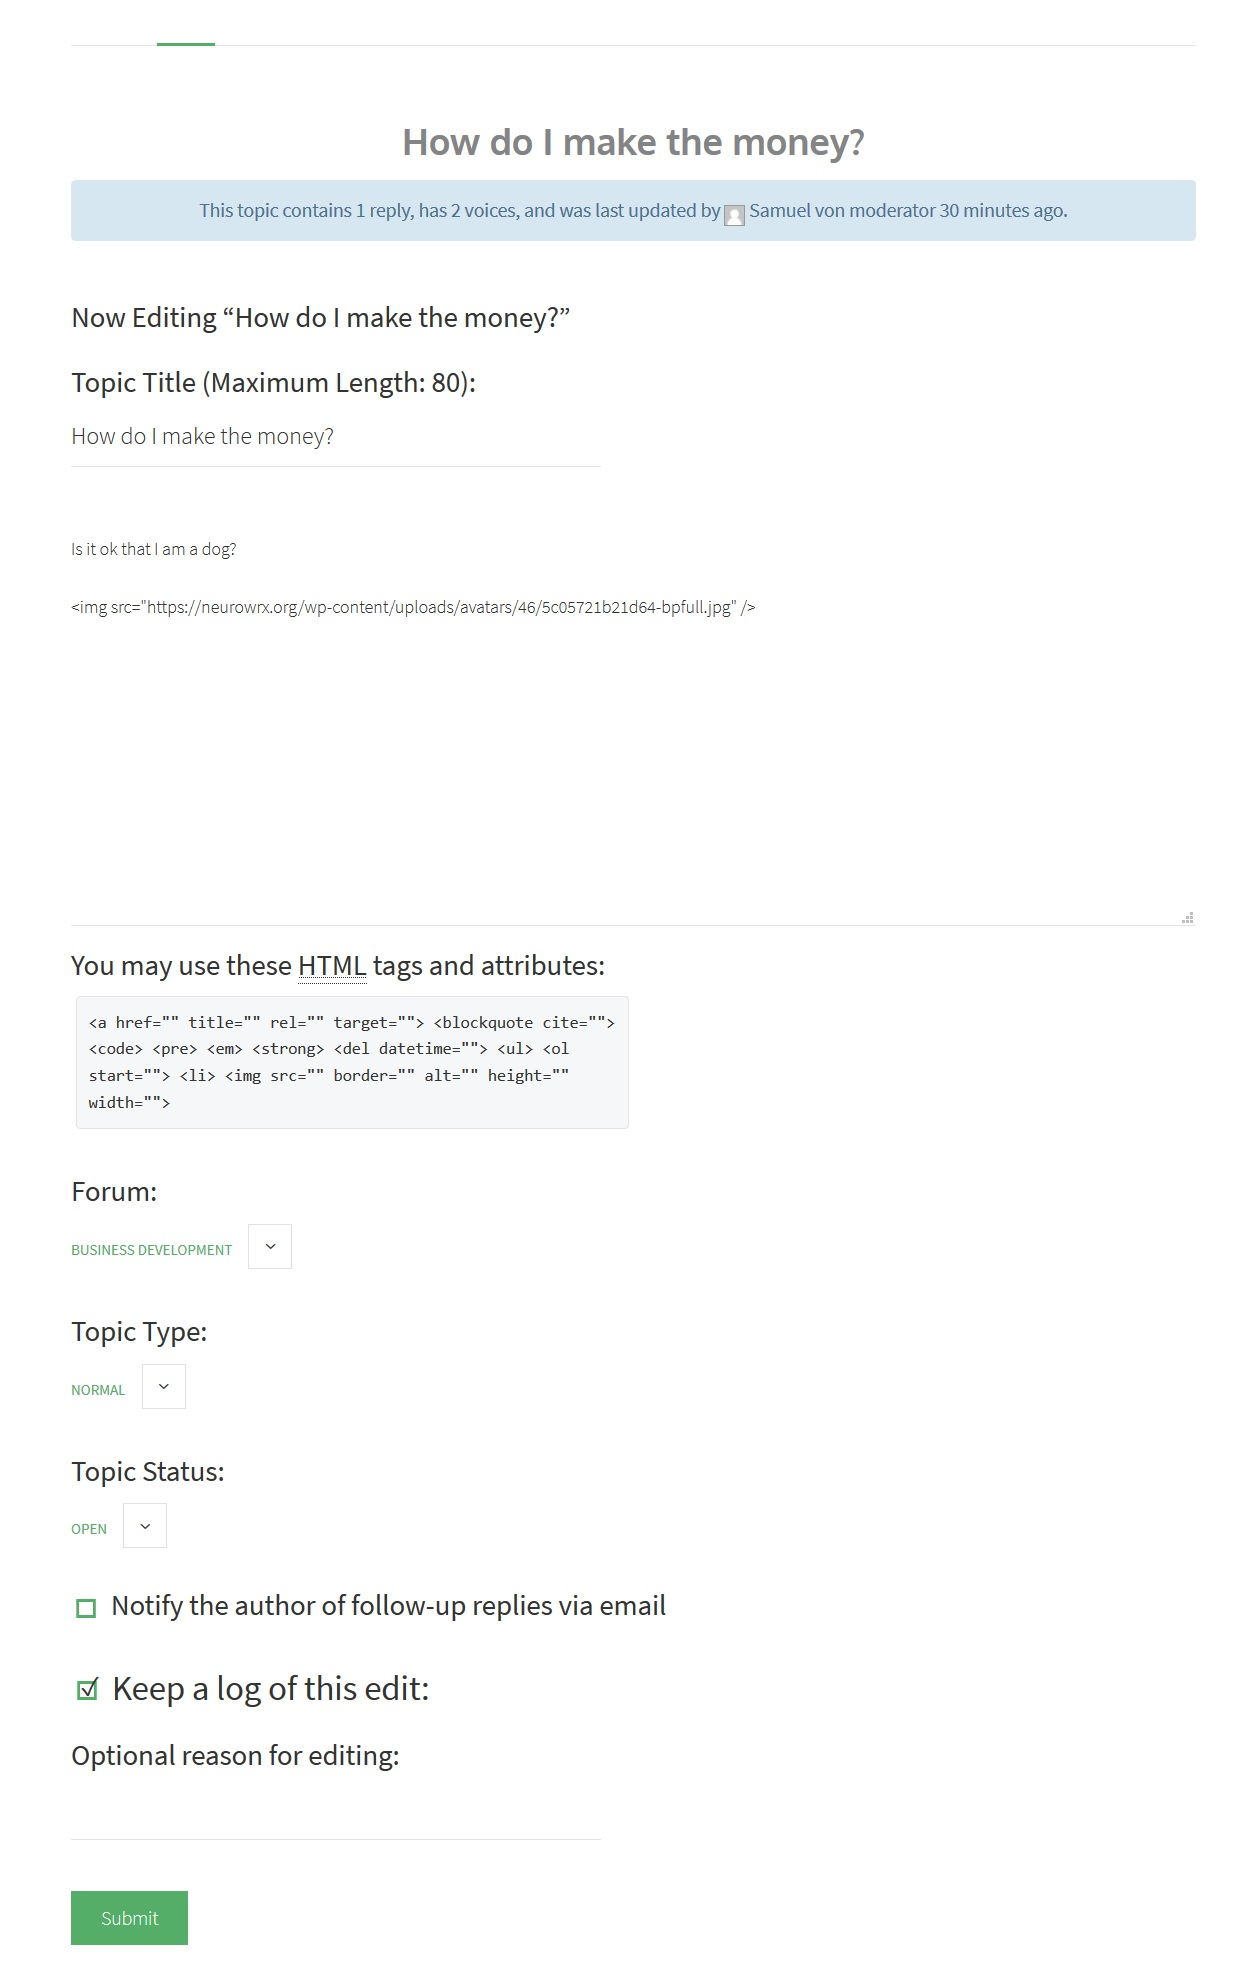
\includegraphics[scale=0.3]{images/editpost.jpg}
    \caption{The post editing window}
    \label{editpost}
\end{figure}

\begin{flushleft}
 If you keep a log of the edit, the fact that the post has been edited will be made known to users who view the post.  If you provide a reason, it will be provided to users who view the post as well (see figure \ref{post edited}). If we add the line "watch me edit your post" and provide "I felt like it" as a reason, the result would look like this (see figure \ref{post edited}). 
\end{flushleft}

\begin{figure}[H]
    \centering
    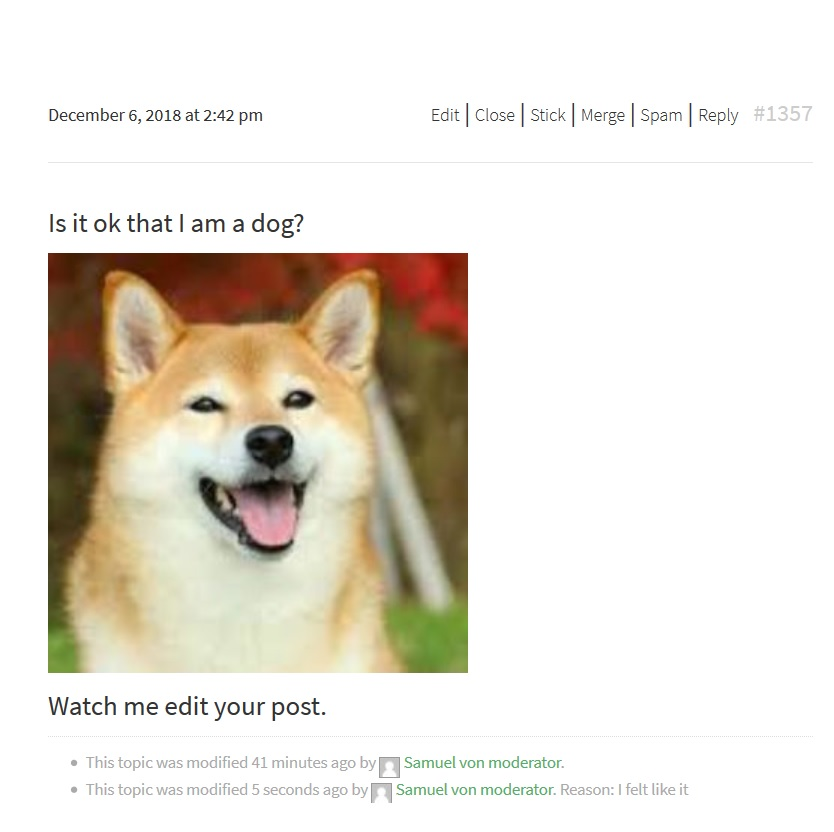
\includegraphics[scale=0.5]{images/postedited.jpg}
    \caption{The post after it has been edited}
    \label{post edited}
\end{figure}

\subsection{Closing Topics}

\begin{flushleft}
Closing topics prevents further replies from being added.  It can be done by clicking on the close link beside the post title in the main forum page, or by changing the topics status to closed in the post editing window.
\end{flushleft}

\subsection{Sticking Topics}
\begin{flushleft}
Stuck topics appear at the top of the list of topics, above all non stuck topics.  It is meant to ensure that everyone has to see them before moving on to other topics further down the list.  It can be engaged by the "stick" link on the main forum page next to the topic title, or with the "Topic Type" dropdown menu in the post editing page.
\end{flushleft}

\subsection{Merging Topics}
\begin{flushleft}
Two topics in the same forum can have all of their replies, subscribers and favouriters combined.  To do this, click the merge link on the main forum page next to the topic title that you wish to merge.  You will be asked to select another topic to merge with (in the same forum) from the dropdown menu and click "submit". 
\end{flushleft}

\begin{flushleft}
Note: this process cannot be undone, and the topic that you select from the dropdown is the one that is subsumed into the other. 
\end{flushleft}

\subsection{Marking Topics as Spam}

\begin{flushleft}
Marking something as spam does not delete it, it just makes it invisible to non moderators.  It can be undone.  To spam, or unspam, a forum topic, view the post in the forum as a moderator and click the link that appears next to the post reply button.
\end{flushleft}




\section{Group Administrators}
Group administrators have elevated access and responsibilities.  They have all of the abilities of a moderator, as discussed in section \ref{Moderators}, in addition to the ability to manage group membership.  The rules governing these things are a matter of policy and not defined in this document.  The following only covers how these things are to be achieved in the application itself. 

\begin{figure}[H]
    \centering
    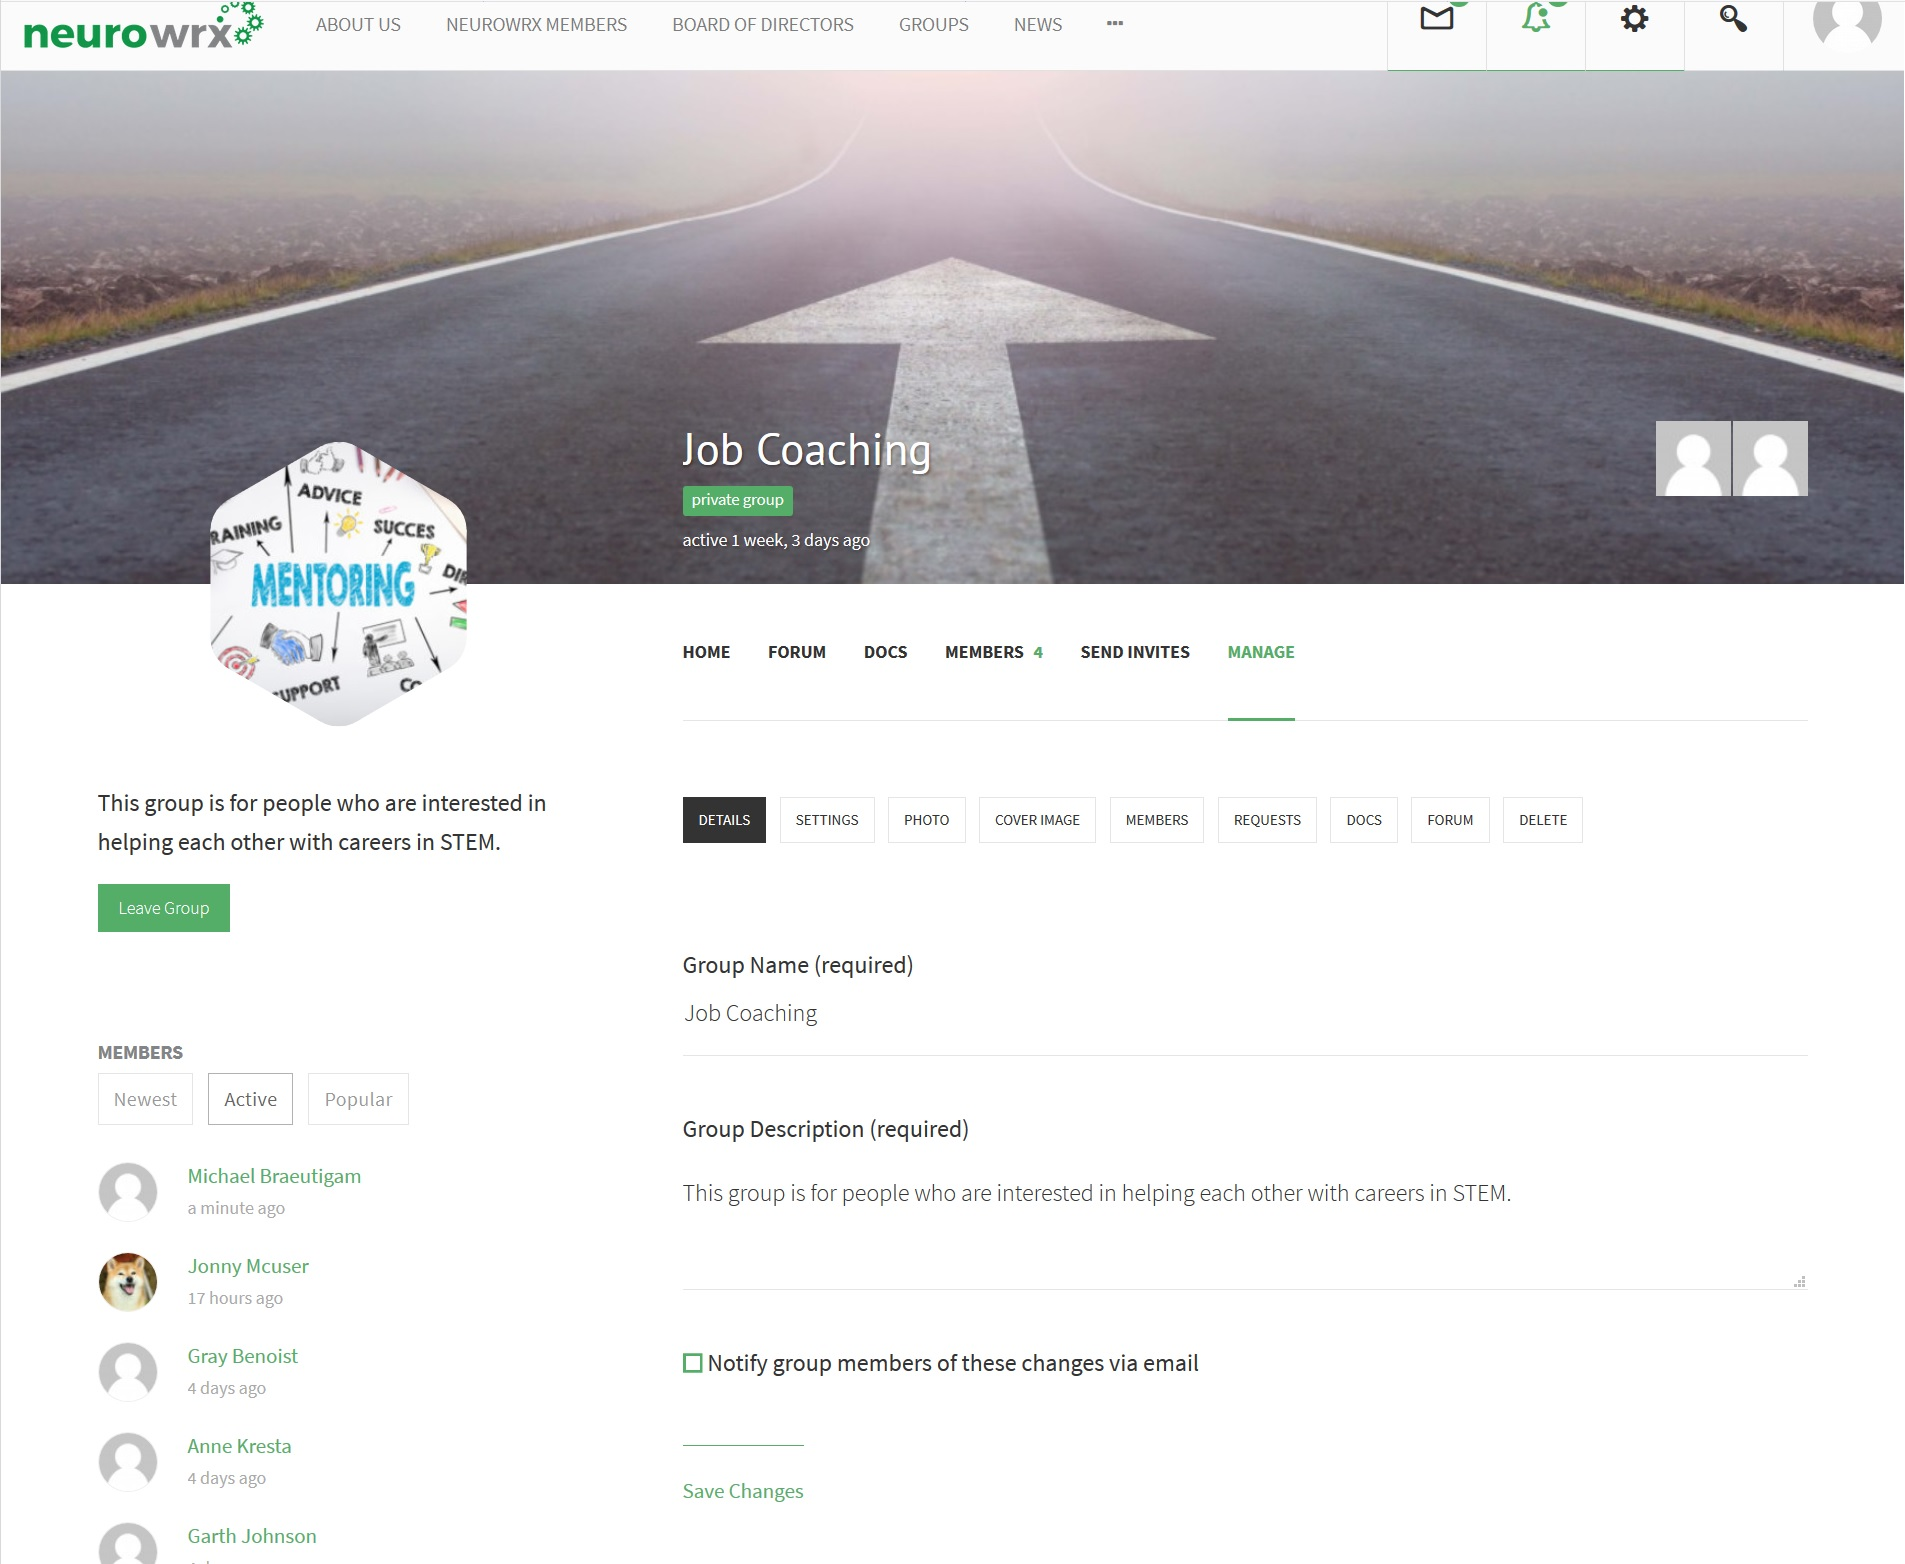
\includegraphics[scale=0.25]{images/groupmanage.jpg}
    \caption{The group management link is visible to group administrators}
    \label{groupmanagelink}
\end{figure}

\subsection{Group Details}

\begin{flushleft}
This page allows the administrator to change the groups name and description.  One can also choose to notify members of these changes via email if they are made.  Simply make the desired changes and click the green "save changes" link at the bottom.  See figure \ref{groupmanagelink}.
\end{flushleft}

\subsection{Group Settings}

\begin{flushleft}
This page allows the administrator to change the privacy settings of a group, as well and control the rules behind who can be invited to join.  By default, groups on this site are intended to be private, but not hidden or public.  If a groups status is changed to public, all of it's associated documents will become publicly visible. See figure \ref{groupsettings}.
\end{flushleft}

\begin{figure}[H]
    \centering
    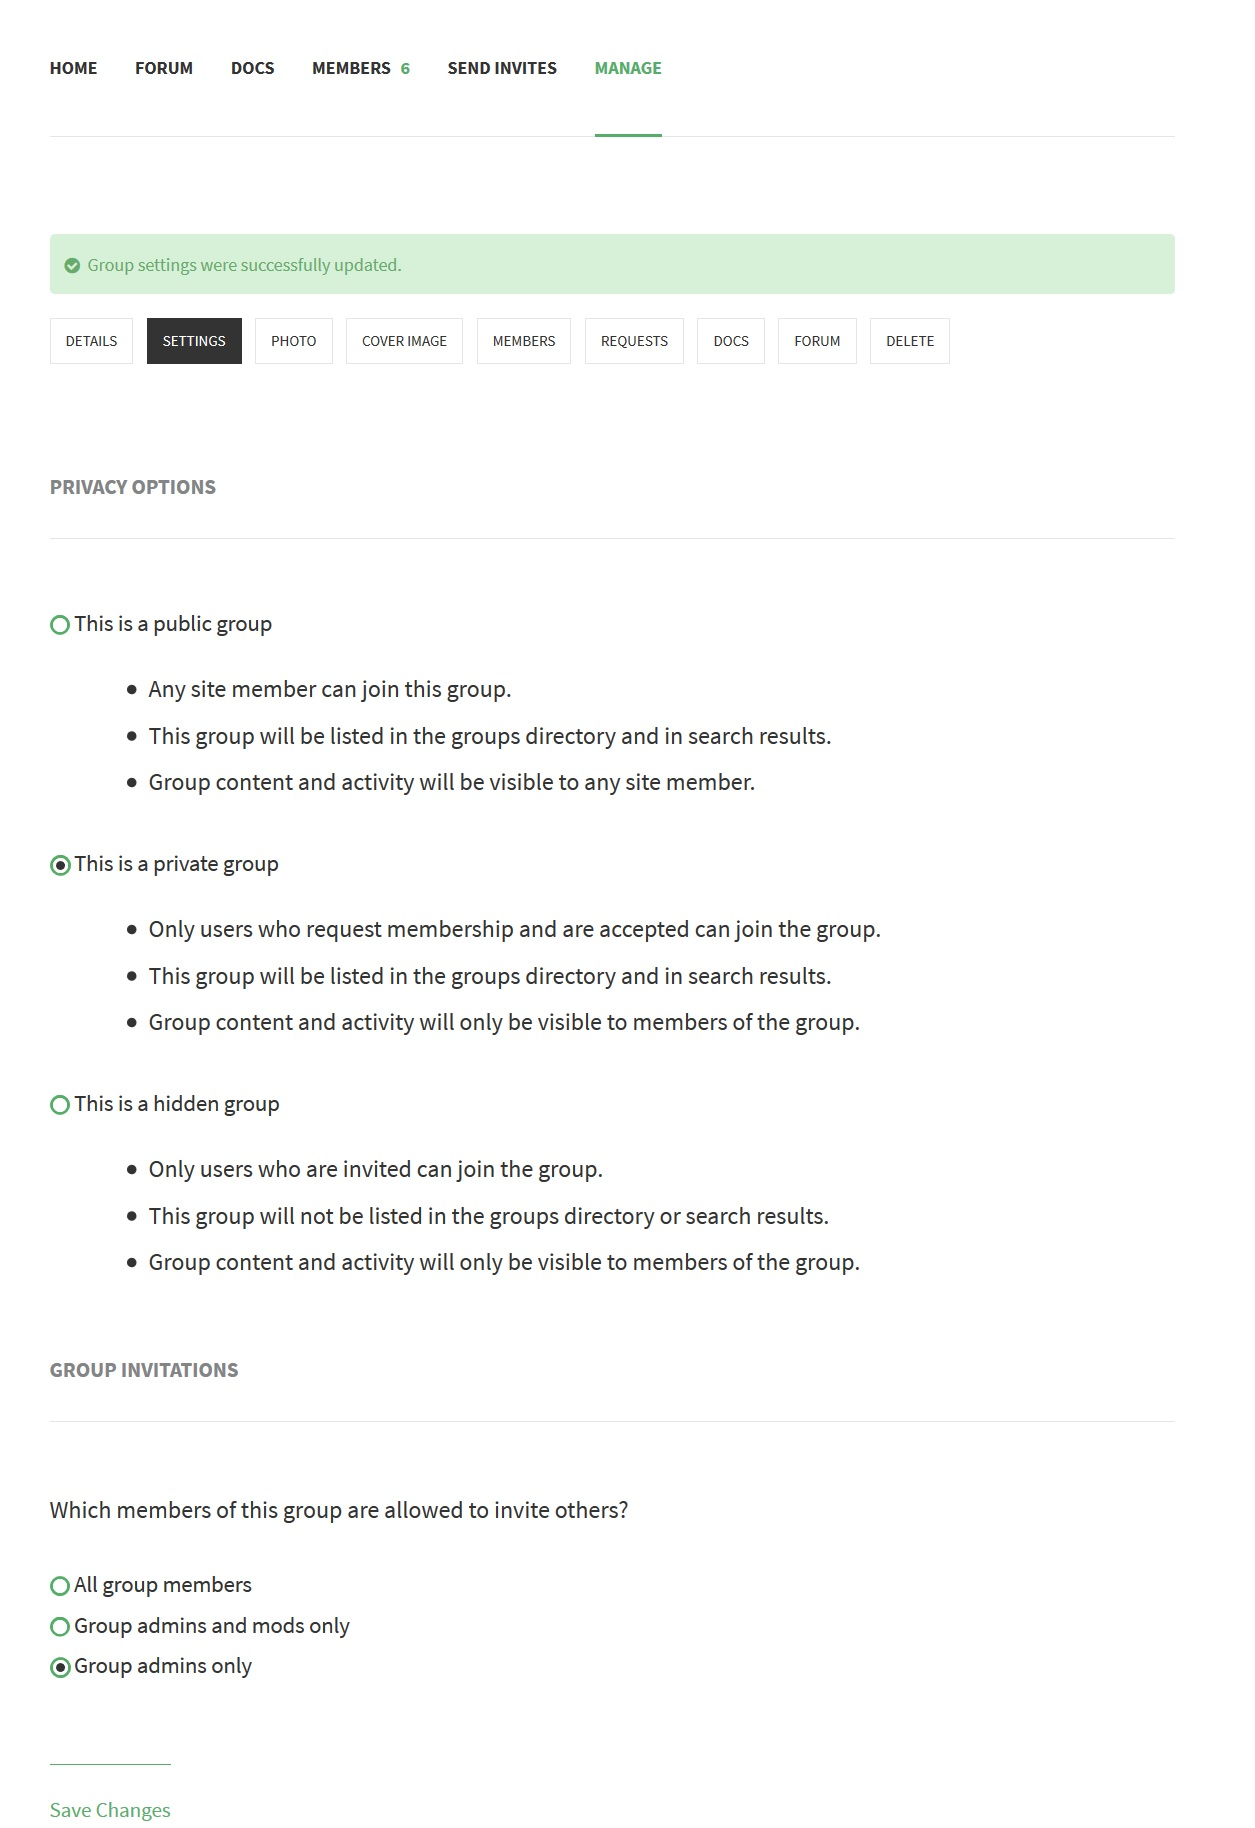
\includegraphics[scale=0.33]{images/groupsettings.jpg}
    \caption{Privacy and invitation settings}
    \label{groupsettings}
\end{figure}

\subsection{Group Photo}

\begin{flushleft}
The group photo is the hexagonal picture that is displayed on the main groups page, among other places.  It can be changed by a group administrator by a similar process as the individual user profile pictures.  To change the group profile picture, click the green select file button, select the file on your local file system, and use the cropping to pick the square subsection of the image that you wish to use.  Once the crop image button is clicked, the change will be made.  Previous profile pictures are not kept anywhere, so the change cannot be undone easily unless the previous photo is manually saved.  See figure \ref{groupphoto}.
\end{flushleft}

\begin{figure}[h]
    \centering
    \subfloat{{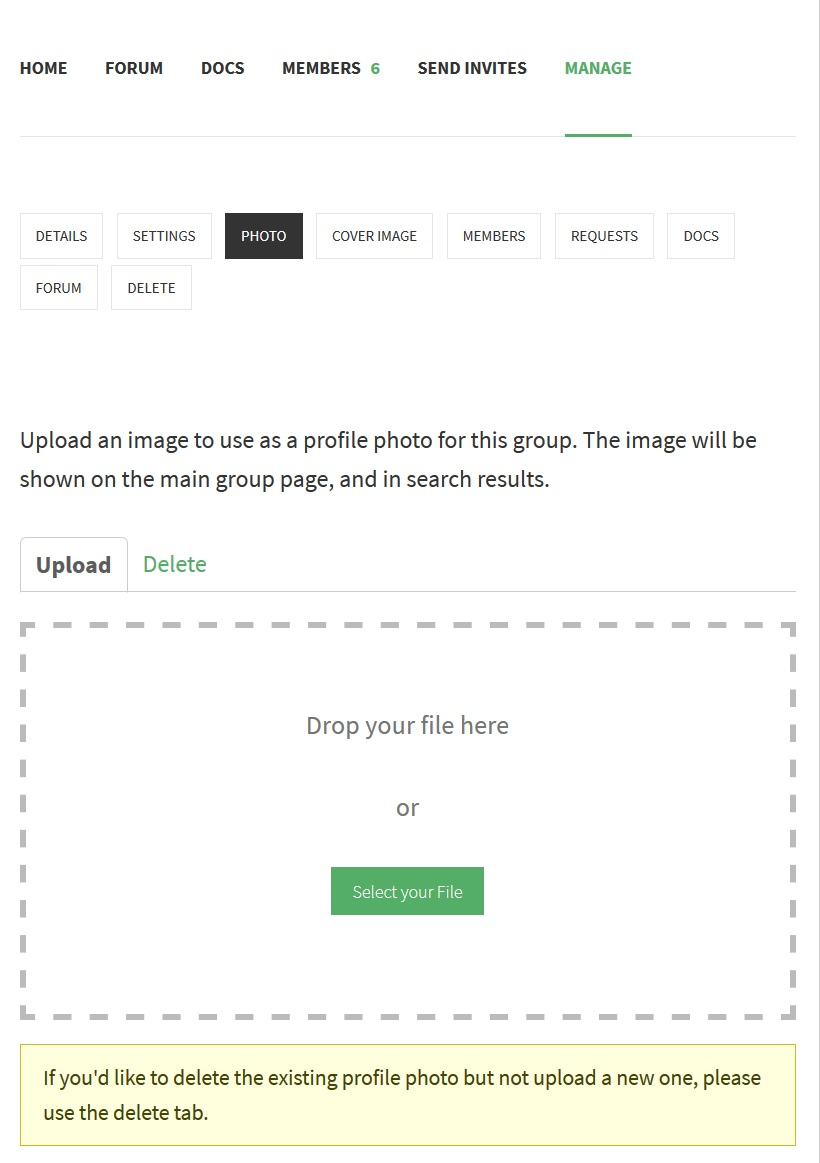
\includegraphics[scale=0.2]{images/groupchangephoto.jpg}}}
    \qquad
    \subfloat{{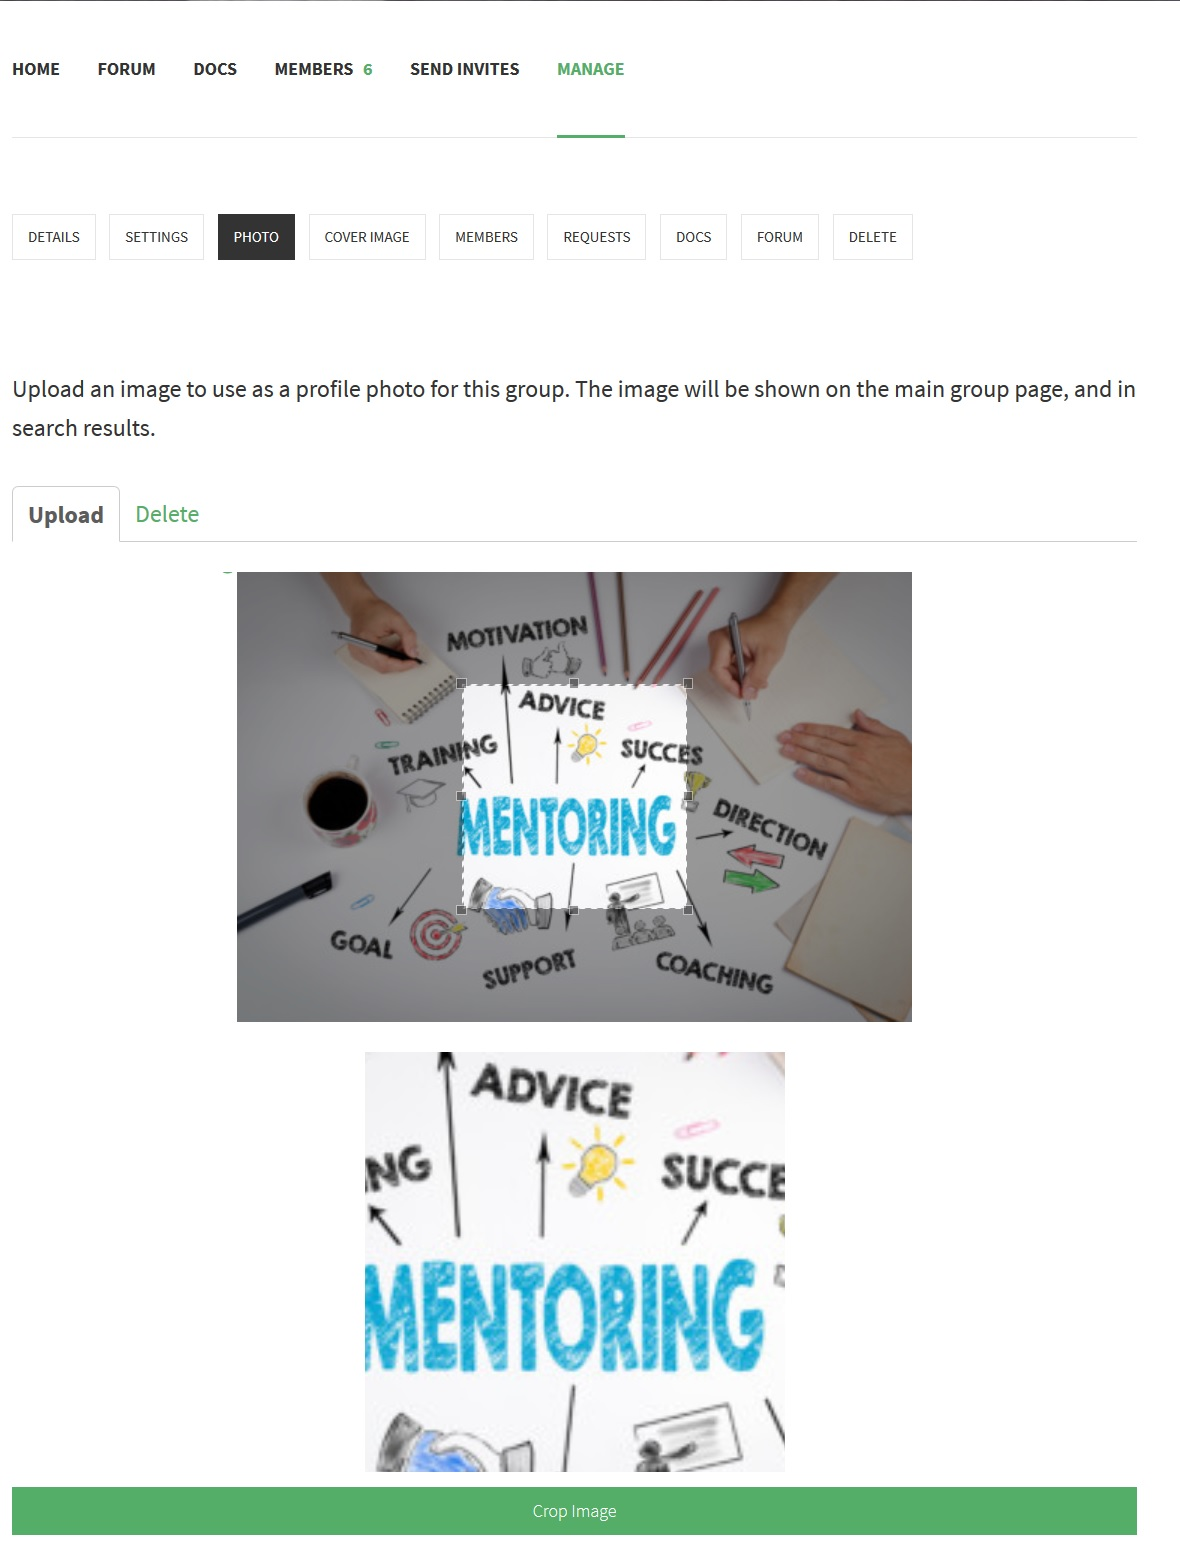
\includegraphics[scale=0.15]{images/groupcropphoto.jpg}}}
    \caption{The two stages of changing the group photo, uploading (left) and cropping (right)}
    \label{groupphoto}
\end{figure}

\subsection{Cover Image}

\begin{flushleft}
The cover image for a group is the wide, thin image that is place below the top panel and underneath the title of all pages specific to a particular group.  In the example below (figure \ref{groupcoverimage}), it is the photograph of the road with an arrow.  
\end{flushleft}

\begin{figure}[H]
    \centering
    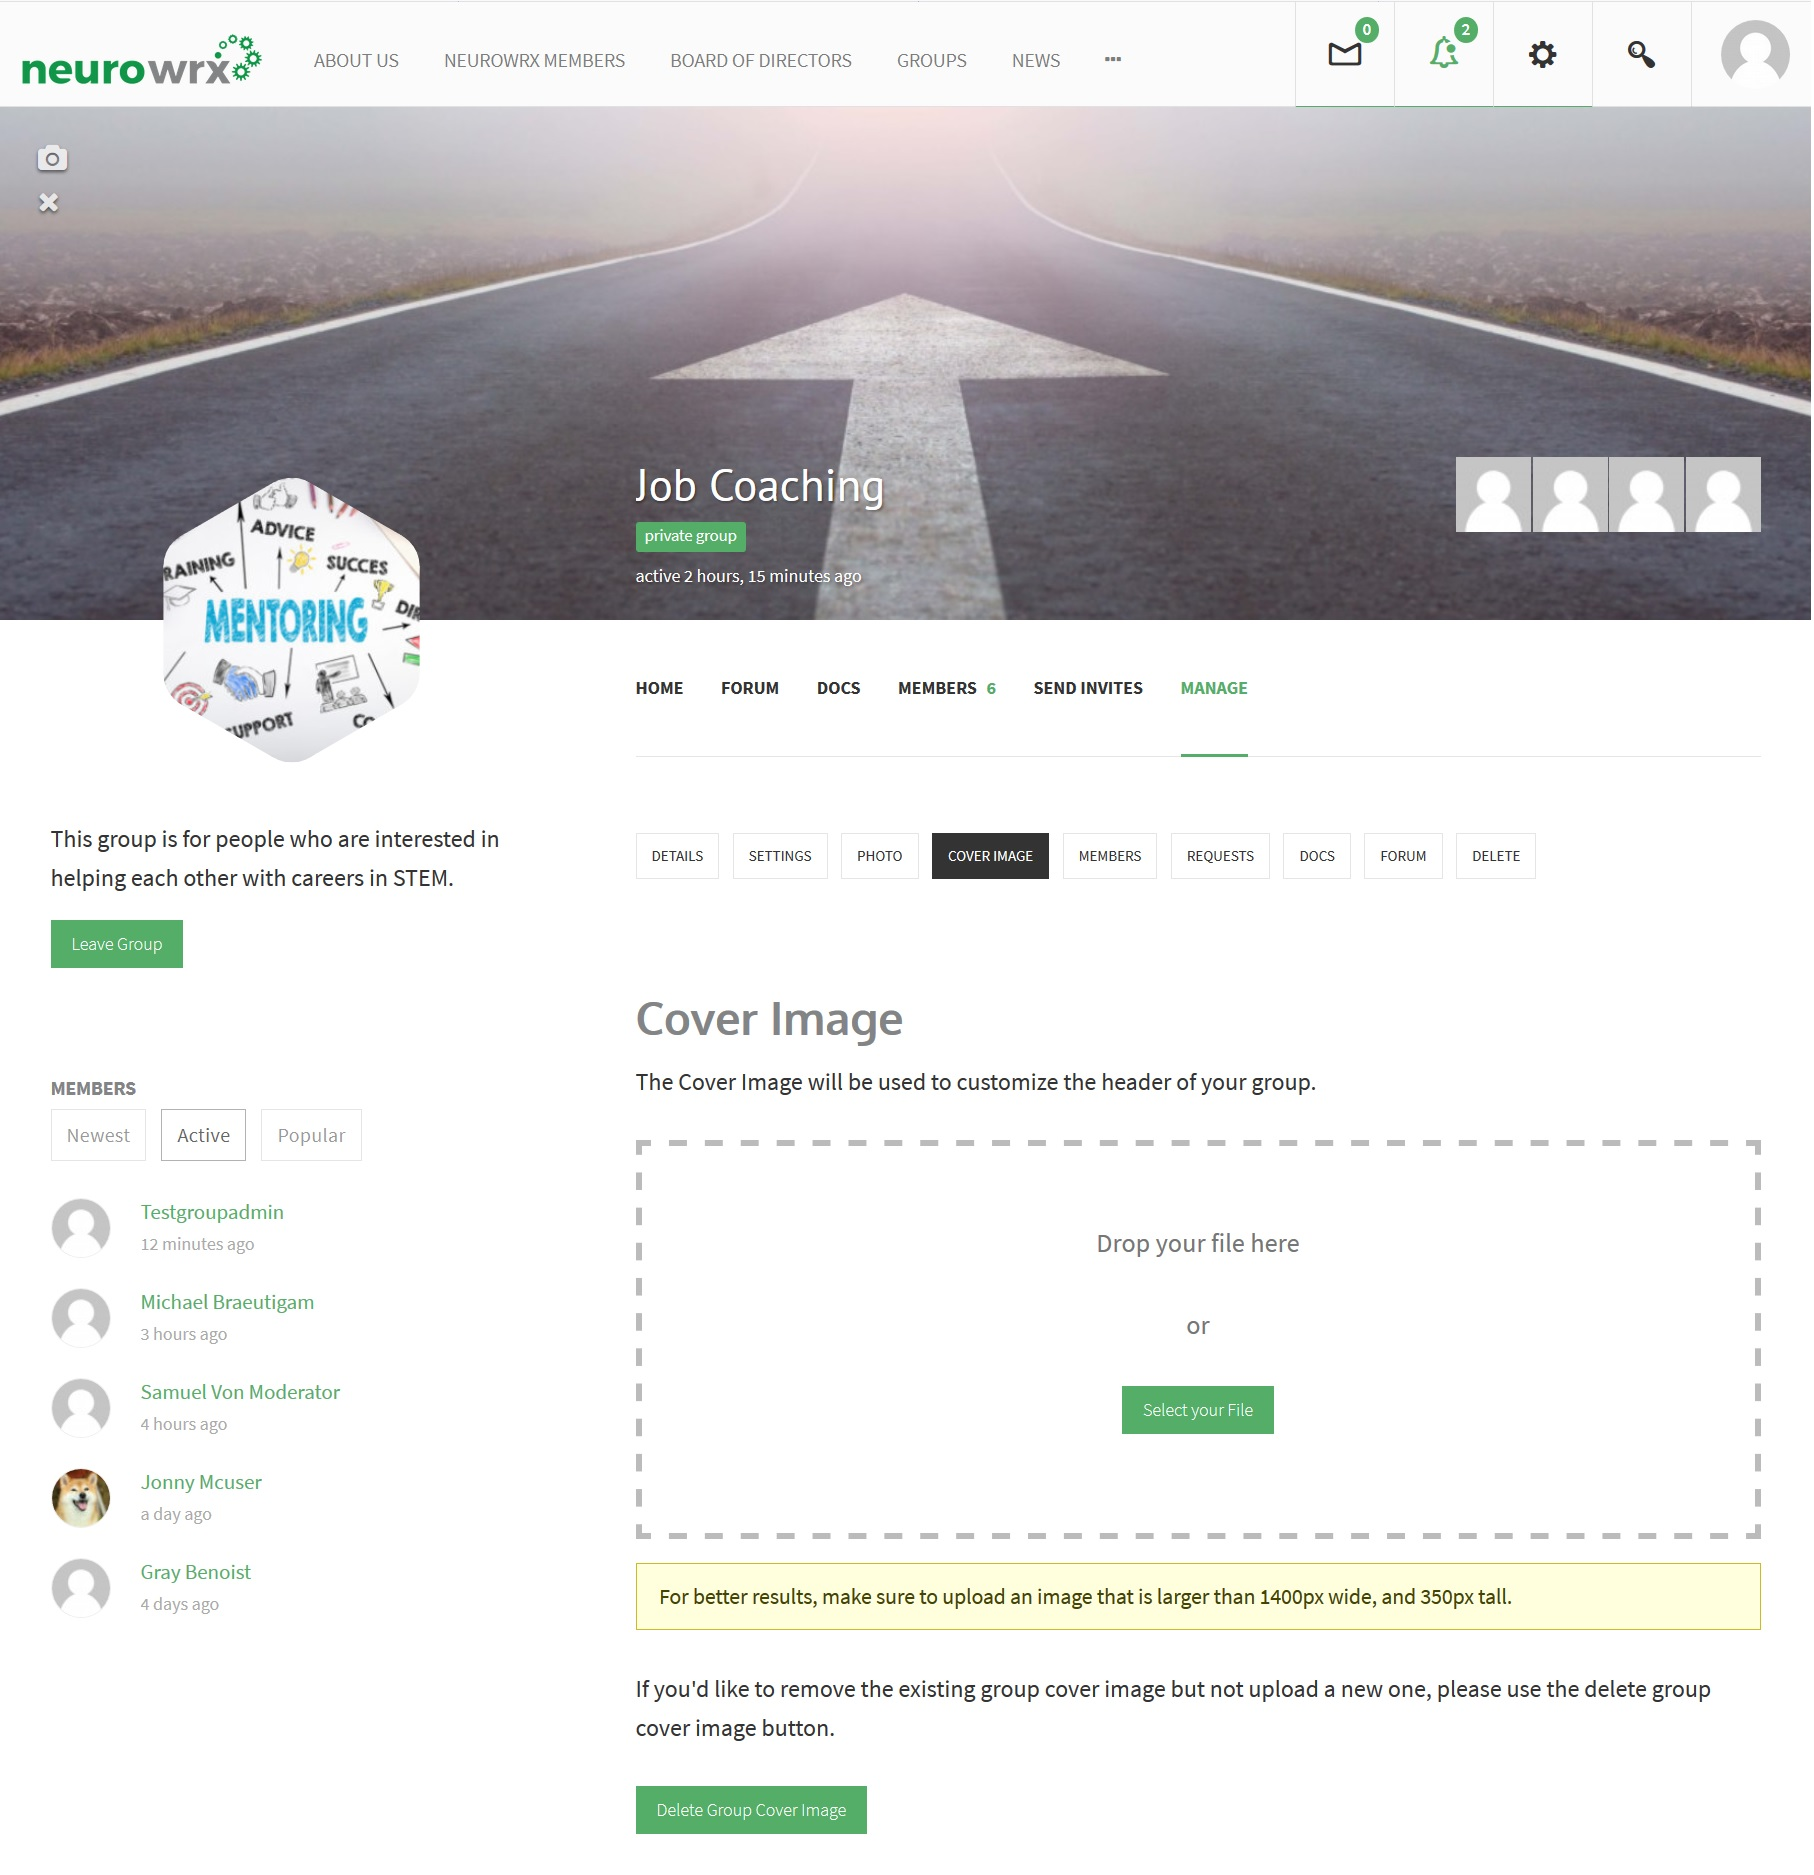
\includegraphics[scale=0.2]{images/groupcoverimage.jpg}
    \caption{The cover image page. Note the camera and "x" at the top left of the photo}
    \label{groupcoverimage}
\end{figure}

\begin{flushleft}
As the text in the yellow box suggests, the resolution of the image is intended to be at least 1400x350 pixels.  The actual portion of the image that is displayed depends on the current window dimensions, with excess width or height being automatically cropped out.  Unlike the profile and group images, these do not ask you to manually crop them with the mouse.  However, just like the profile images and group image, previous images are not saved, so if one desires to merely test a new image, it is recommended that the current one be manually saved.  You are not obligated to use a cover image, and the current one can be deleted by clicking the green button at the bottom of the page. 
\end{flushleft}

\begin{flushleft}
There is also a semi transparent camera and "x" in the top left corner of the cover image that is visible in administrator mode.  These two buttons also allow you to remove or change the cover image.
\end{flushleft}

\subsection{Members}
\begin{flushleft}
The members page of the group management function allows an administrator to promote, demote, remove or ban group members.  It does not enable you to accept requests, which is handled elsewhere.  Administrators or moderators cannot be removed or banned unless first demoted to ordinary members.  It is possible to demote one's self, and any administrator can remove the administrator status of any other administrator. 
\end{flushleft}

\begin{flushleft}
Banning a member is similar to removing them, except that they cannot attempt to rejoin the group until they are unbanned.  They can only be unbanned by a site administrator on the wordpress dashboard.  The ban is specific to the group, and does not affect their status or abilities on the rest of the site.  
\end{flushleft}

\begin{figure}[H]
    \centering
    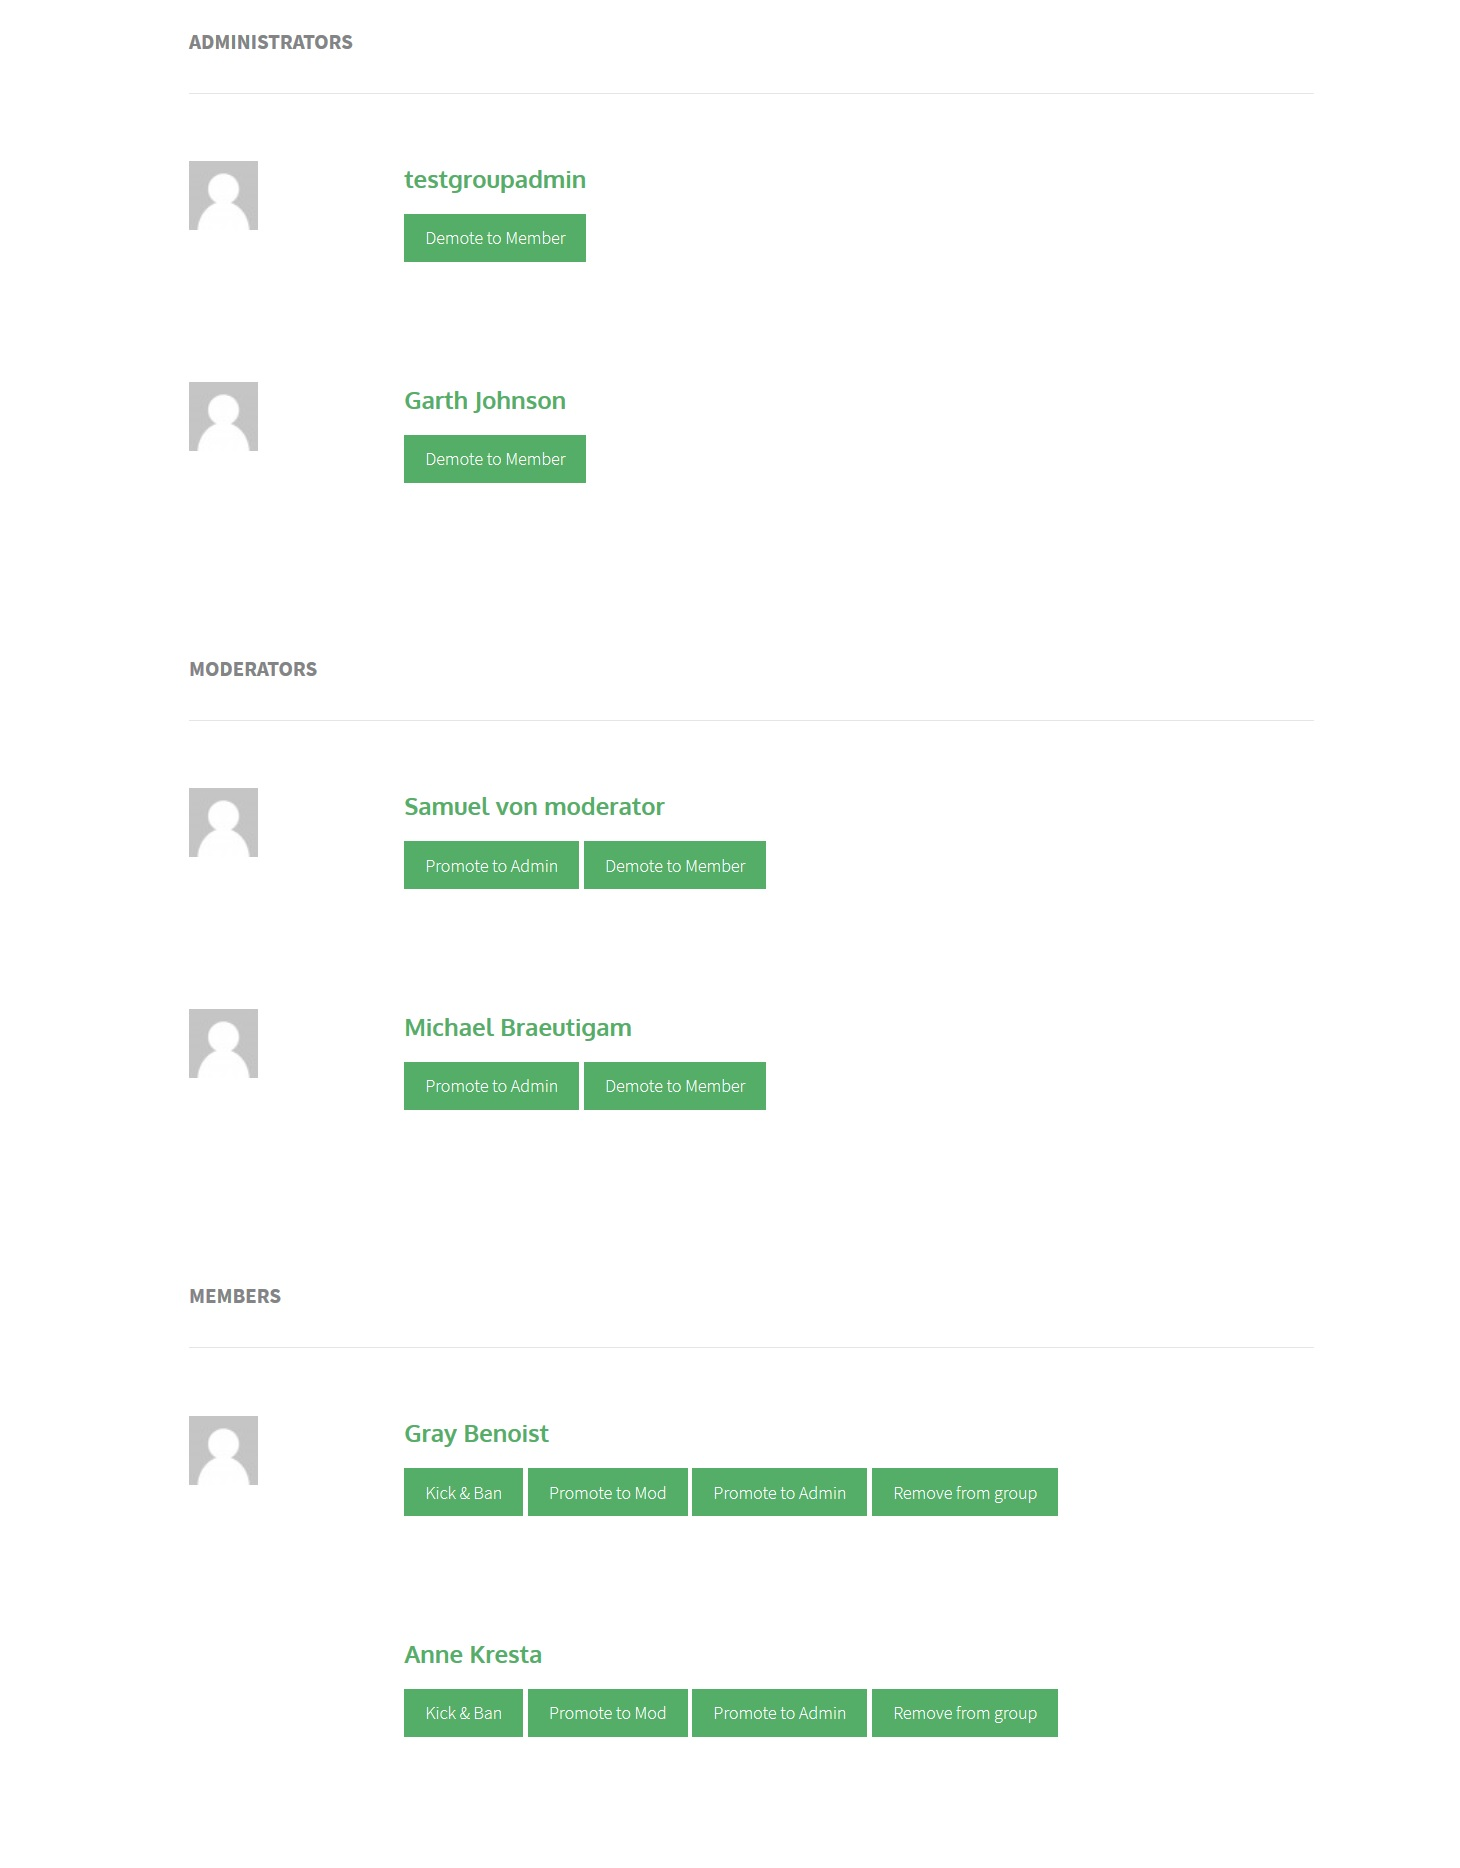
\includegraphics[scale=0.4]{images/managemembers.jpg}
    \caption{The member management page}
    \label{managemembers}
\end{figure}

\begin{flushleft}

All of the member management actions available with respect to a given user are listed beside their name on the list, and are determined by the rank of their membership (see figure \ref{managemembers}).  You will be asked to confirm any action that you take. 

\end{flushleft}

\subsection{Join Requests}


\begin{figure}[H]
    \centering
    \includegraphics[scale=0.5]{images/memrequest.jpg}
    \caption{The join request page}
    \label{memrequest}
\end{figure}

\begin{flushleft}
Join requests can either be accepted or rejected as the administrator wishes.  If they are rejected they can be resent by the applicant.  They are accepted or rejected by clicking the corresponding button under the users profile picture in the join request list (see figure \ref{memrequest}).
\end{flushleft}


\subsection{Documents}

\begin{flushleft}
At this time, only group administrators have the ability to create new documents.  To do this, go to the home page of a particular group, and then click the docs link at the top of the group's page (see figure \ref{adminsdocspage}).
\end{flushleft}

\begin{figure}[H]
    \centering
    \includegraphics[scale=0.5]{images/docspage.jpg}
    \caption{The documents page as a group admin sees it}
    \label{adminsdocspage}
\end{figure}

\begin{flushleft}
As you can see, there is a green "Create New Doc" button on the right available to administrators. If we click this, we are brought to the document creation form (see figure \ref{doccreationform}).  
\end{flushleft}

\begin{figure}[H]
    \centering
    \includegraphics[scale=0.5]{images/doccreationform.jpg}
    \caption{The document creation form}
    \label{doccreationform}
\end{figure}

\begin{flushleft}
This form has many features.  In addition to being able to choose the title and create the (initial) content of the document in an MS word-like editor, you can attach relevant files.  Further down the form, you can choose which group the document will be associated with, which by default, is the group whos page you were on when you clicked the create document link.  
\end{flushleft}

\begin{flushleft}
In the access section, you can set the read and edit access permissions of the document, as well as read and access permissions of the comments that can be made on the document. You can also view who controls the history of the document.  By default, these are all set so that all members of a given group can perform all of the above mentioned functions.  In practice, it is likely that you will often want to restrict edit permission to moderators or admins of a particular group.  You can change access permissions on a document at any time if you are an adminstrator for a group, regardless of whether or not you created the original document. 
\end{flushleft}

\begin{flushleft}
There is also a section for adding tags to a doc to help people find it using the search bar at the top of the site (assuming they have the necessary privileges to view it).  Simply add or edit the comma separated list of words or phrases to assist in the categorization of this document (if you wish to do so).
\end{flushleft}

\begin{flushleft}
Finally, the document parent function forces another document to be displayed at the bottom of the page whenever this document is viewed, and a link to the child to be displayed at the bottom of the page whenever the parent is viewed.  When a parent to a document is added, it's title is selected from a list of existing documents on the site.
\end{flushleft}

\begin{flushleft}
Once the admin is satisfied with the contents of the form, clicking the save button will create the document. 
\end{flushleft}

\subsection{Forum}
\begin{flushleft}
In addition to the ordinary moderation powers described in section \ref{Moderators}, administrators have the power to instantly put any post they see in the trash.  Once there, the content can only be restored by a site administrator. The trash button appears next to the reply butten in the regular post view window.
\end{flushleft}

\subsection{Delete Group}

\begin{flushleft}
The administrator of a group can delete it at any time.  This can potentially result in the loss of valuable content, and cannot be undone from within the application.  It would require restoring the website from a backup, which might entail the loss of days worth of activity.  Not to be trifled with. 
\end{flushleft}

\section{Site Administrators}

\begin{flushleft}
Site administrators are given full access to the wordpress dashboard, and are able to make essentially arbitrary changed to the website.  They have the ability to manually add or remove any user, and any piece of contend, as well as add pages and functionality to the site.
\end{flushleft}

\begin{flushleft}
The dashboard can be accessed from the dropdown menu under your profile picture if you are made a site administrator.  The use of the wordpress console is largely beyond the scope of this document.
\end{flushleft}

\bibliography{codes_impact}
\bibliographystyle{plainnat}
\end{document}